%%%%%%%%%%%%%%%%%%%%%%%%%%%%%%%%%%%%%%%%%%%%%%%%%%%%%%%%%%%%%%%%%%%%%%
% utdiss.doc
%%%%%%%%%%%%%%%%%%%%%%%%%%%%%%%%%%%%%%%%%%%%%%%%%%%%%%%%%%%%%%%%%%%%%%
\documentclass[12pt, a4paper]{report}


\usepackage{graphicx}

%\usepackage{ncku/pdf}


%\usepackage{style/rotating}

\usepackage{style/macros}

%\usepackage{style/psfig}

%\usepackage{epsfig}

\usepackage{latexsym}

\usepackage{style/utdiss}

%\usepackage{hyperref}


%加這個就可以設定字體
\usepackage{fontspec}
%使用xeCJK,其他的還有CJK或是xCJK
\usepackage{xeCJK}

% Set english font
\setmainfont{Times New Roman} % In Windows
%\usepackage{times} % In *nix 

%設定中英文的字型
%字型的設定可以使用系統內的字型,而不用像以前一樣另外安裝
\setCJKmainfont{標楷體}

%中文自動換行
\XeTeXlinebreaklocale "zh"

%文字的彈性間距
\XeTeXlinebreakskip = 0pt plus 1pt

%設定段落之間的距離
\setlength{\parskip}{0.3cm}

%設定行距
\linespread{1.5}\selectfont







%\newtheorem{theorem}{Theorem}
%\newtheorem{lemma}{Lemma}
%\newtheorem{example}{Example}
%\newtheorem{corollary}{Corollary}

%%%%%%%%%%%
% Spacing %
%%%%%%%%%%%

% According to the Dissertation Preparation Guideline,
% the main texts should be either doublespaced or
% one-&-half-spaced. Quoted texts may be either
% doublespaced, one-half-spaced, or singlespaced.
%
% Main Text Spacing: Default = \doublespacing
%
%    One-&-Half-Spacing (Main Text)
%          \onehalfspacing
%
%    Single-Spacing (Main Text)
%          \singlespacing
%
% Quoted Text Spacing: Default = doublespacing
%
%    One-&-Half-Spacing (Quoted Text)
%          \onehalfspacequote
%
%    Single-Spacing (Quoted Text)
%          \singlespacequote

%%%%%%%%%%%%%%%%%%%%%%%%%%%%%%%%%%%%%%
% Table of Contents Table Adjustment %
%%%%%%%%%%%%%%%%%%%%%%%%%%%%%%%%%%%%%%

% \longtocentry         % Only if there are 10 or more sections,
            % 10 or more subsections for a section,
            % etc. etc.
            % Usually, NOT required.

%%%%%%%%%%%%%%%%%%%%%%%%%%%%%%%%%%%
% DATA OF AUTHOR AND DISSERTATION %
%%%%%%%%%%%%%%%%%%%%%%%%%%%%%%%%%%%
\title{Bus-Pin-Aware Bus-Driven Floorplanning} % Required

\author{Po-Hsun Wu}            % Required
%
% Replace the dots in the command by your full name.
% Make it combination of lower and uppercases
% e.g., \author{Dorothy Kay Shoemaker}

%
% Replace the dots in the above command by your thesis title,
% e.g., `\title{A Take of Gnus, Gnats and \\ Armadillos}'.
% If the title consists of more than one line,
% it should be in inverted pyramid form. You have to specify the
% line breakings by \\ commands.

\previousdegrees{B.S, M.S.}      % Optional if use default
%
% The abbreviated form of your previous degree(s).
% e.g., \previousdegrees{B.S., MBA}
% The default value is `B.S., M.S.'

\degree{DOCTOR OF PHILOSOPHY} % Optional if use default
%
% The degree sought as given in the Graduate Catalogue.
% Capital letters are recommended.
% e.g., `\degree{DOCTOR OF BUSINESS ADMINISTRATION}'
% The default value is `DOCTOR OF PHILOSOPHY' for dissertation.

\degreeabbr{PH.D.}       % Optional if use default
%
% The abbreviated form of your degree sought.
% e.g., `\degreeabbr{DBA}'
% The default is `Ph.D.'
% Note: the abbreviated form is not automatically
%       generated from \degree{...}.
%       If you enter \degree{...}, you should enter
%   \degreeabbr{...}, too.

\graduationmonth{June}        % Optional if let the system generate
%
% Graduation month, in the form as `\graduationmonth{May}'.
% The default value (either May, August, or December)
% is guessed according to the time of running LaTeX
% Do not abbreviate.
% Note: either May, August, or December
%              ^^^  ^^^^^^     ^^^^^^^^

\graduationyear{2010}       % Optional if let the system generate
%
% Graduation year, in the form as `\graduationyear{1991}'.
% The default value is guessed according to the time of running LaTeX.
% 4 (not 2) digit number

\address{No.60-1, Aly. 5, Ln. 88, Min¡Šan W. Rd., Xinzhuang City, Taipei County 242, Taiwan (R.O.C.)} % Required
%
% Your *permanent* (not local) address.
% Use \\ to separate address lines.
% e.g., `\address{4533 Avenue A\\ Austin, Texas 78751}'.

%\typist{the author}            % Optional if use default
%
% The name(s) of typist(s), put `the author' if you do it yourself.
% E.g., `\typist{Maryann Hersey and the author}'.
% The default value is `the author'.

% The name(s) of your supervising professor(s). Up to 3
% List the first/second one in []'s and the last one in {}
%\supervisor[first][second]{third}

\supervisor{Tsung-Yi Ho}      % Required

\committeesize{3}
%
% x = The number of supervisors
% y = The size of your supervising committee including supervisor(s)
% e.g., `\committeesize{6}'.              ^^^^^^^^^^^^^^^^^^^^^^^
% The default values -- x = 1; y = 5
% Note: x <= 3

% 增強功能型頁楣 / 頁腳套件
\usepackage{fancyhdr}  % 借用此套件來擺放浮水印 
% (佔用了 central header)
% 不需要浮水印的使用者仍可利用此套件,產生所需的 header, footer
%
% 啟動 fancy header/footer 套件
\pagestyle{fancy}
\fancyhead{}  % reset left, central, right header to empty
\fancyfoot[C]{\thepage} %中間 footer 擺放頁碼
\renewcommand{\headrulewidth}{0pt} % header 的直線; 0pt 則無線

% 如果不需要任何浮水印,則請把下列介於 >>> 與 <<< 之間
% 的文字行關掉 (行首加上百分號)
%% 浮水印 >>> 
%
% this file is encoded in utf-8


% 增強功能型頁楣 / 頁腳套件
\usepackage{fancyhdr}  % 借用此套件來擺放浮水印 
% (佔用了 central header)
% 不需要浮水印的使用者仍可利用此套件,產生所需的 header, footer
%
% 啟動 fancy header/footer 套件
\pagestyle{fancy}
\fancyhead{}  % reset left, central, right header to empty
\fancyfoot[C]{\thepage} %中間 footer 擺放頁碼
\renewcommand{\headrulewidth}{0pt} % header 的直線; 0pt 則無線






% v2.02 (Sep. 12, 2012)
% 如果浮水印不是全篇需要,請把下列介於 >>> 與 <<<
% 的「全篇浮水印專用碼」關掉 (行首加百分號)
% 參考自 Keith Reckdahl 寫的 "Using Imported Graphics in LATEX2e" (epslatex.pdf) p.39
% 如果只有特定頁需要浮水印
% 則依該頁屬性使用下列之一的命令 
% 普通頁命令 \thispagestyle{WaterMarkPage}
% plain 頁命令 \thispagestyle{PlainWaterMarkPage}
% empty 頁命令 \thispagestyle{EmptyWaterMarkPage}


% 將重複使用的浮水印章
% 圖檔是 my_watermark.xxx
% 副檔名可以不加,可以是 latex 系統能處裡的任何格式:pdf, gif, png, jpg, eps, ...
% 某些圖檔格式在某些工作流程可能需要作前置處裡。
% 例如,pdflatex 無法直接處理 eps 檔
%  latex + dvipdfmx 無法直接處理 pdf, gif, png, jpg, 需要用 ebb 小工具程式
%  對圖檔產生 .bb 對應檔。
%
% 寬為 5.1 cm
\newsavebox{\mywatermark}
\sbox{\mywatermark}{
\includegraphics[keepaspectratio,%
width=5.1cm]{./ncku/watersymbol.jpg}}


% 將 central header 擺放浮水印的巨集指令
\newcommand{\PlaceWaterMark}{\fancyhead[C]{\setlength{\unitlength}{1in}%
\begin{picture}(0,0)%
\put(-1,-5){\usebox{\mywatermark}}% 圖檔擺放的位置座標
\end{picture}}%
}

\fancyhead{}  % reset left, central, right header to empty
%% 如果不需整篇論文都要浮水印
%% 則下面  >>> 與 <<< 之間的程式碼請關閉
%% >>> 全篇浮水印
\PlaceWaterMark  % 每一頁都有浮水印 (除了 plain、empty 頁以外)

% 重新定義 plain 頁面
% 每張 plain 頁面 (每一章的第一頁) 也加浮水印

\fancypagestyle{plain}{%
\fancyhead{}%
\PlaceWaterMark%
\fancyfoot{}%
\fancyfoot[C]{\thepage}
\renewcommand{\headrulewidth}{0pt}%
\renewcommand{\footrulewidth}{0pt}%
}
%% <<< 全篇浮水印

%% 如果只有一、兩頁需要有浮水印
%% 可以在該頁 (有頁碼) 使用 \thispagestyle{WaterMarkPage}
%% 此命令不影響原有的 header、footer
\fancypagestyle{WaterMarkPage}{%
\PlaceWaterMark%
}

%% 如果只有一、兩頁 plain 頁需要有浮水印 (如 摘要、自傳等)
%% 可以在該頁 (有頁碼) 使用 \thispagestyle{PlainWaterMarkPage}
%% 只有頁碼與浮水印,沒有其他的 header、footer
%% 等同於 plain page style + water mark
\fancypagestyle{PlainWaterMarkPage}{%
\fancyhead{}%
\PlaceWaterMark%
\fancyfoot{}%
\fancyfoot[C]{\thepage}
\renewcommand{\headrulewidth}{0pt}%
\renewcommand{\footrulewidth}{0pt}%
}

%% 如果只有一、兩頁 empty 頁需要有浮水印 (如封面、書名頁)
%% 可以在該頁 (無頁碼) 使用 \thispagestyle{EmptyWaterMarkPage}
%% 等同於 empty page style + water mark
\fancypagestyle{EmptyWaterMarkPage}{%
\fancyhead{}%
\PlaceWaterMark%
\fancyfoot{}%
\renewcommand{\headrulewidth}{0pt}%
\renewcommand{\footrulewidth}{0pt}%
}

%% <<< 浮水印

%\includeonly{tex/finale}


\begin{document}







% default variables definitions
% 此處只是預設值,不需更改此處
% 請更改 my_names.tex 內容
\newcommand\cTitle{論文題目}
\newcommand\eTitle{MY THESIS TITLE}
\newcommand\myCname{胡庭瑜}
\newcommand\myEname{Ting-Yu Hu}
\newcommand\advisorCnameA{陳朝鈞博士}
\newcommand\advisorEnameA{Dr.~Chao-Chun~Chen}
\newcommand\advisorCnameB{莊坤達博士}
\newcommand\advisorEnameB{Dr.~Kun-Da~Chuang}
\newcommand\advisorCnameC{王鼎超博士}
\newcommand\advisorEnameC{Dr.~Ding-Chau~Wang}
\newcommand\univCname{成功大學}
\newcommand\univEname{National Cheng Kung University}
\newcommand\deptCname{製造資訊與系統研究所}
\newcommand\fulldeptEname{Institue of Manufacturing Information and Systems}
\newcommand\deptEname{Inst. of Manuf. Info. \& Sys.}
\newcommand\collEname{College of Electrical Engineering and Computer Science}
\newcommand\degreeCname{碩士}
\newcommand\degreeEname{Master of Engineering}
\newcommand\cYear{一○一}
\newcommand\cMonth{七}
\newcommand\eYear{2012}
\newcommand\eMonth{June}
\newcommand\ePlace{Tainan, Taiwan}


 % user's names; to replace those default variable definitions
%
% this file is encoded in utf-8
% v2.02 (Sep. 12, 2012)
% 填入你的論文題目、姓名等資料
% 如果題目內有必須以數學模式表示的符號,請用 \mbox{} 包住數學模式,如下範例
% 如果中文名字是單名,與姓氏之間建議以全形空白填入,如下範例
% 英文名字中的稱謂,如 Prof. 以及 Dr.,其句點之後請以不斷行空白~代替一般空白,如下範例
% 如果你的指導教授沒有如預設的三位這麼多,則請把相對應的多餘教授的中文、英文名
%    的定義以空的大括號表示
%    如,\renewcommand\advisorCnameB{}
%          \renewcommand\advisorEnameB{}
%          \renewcommand\advisorCnameC{}
%          \renewcommand\advisorEnameC{}

% 論文題目 (中文)
\renewcommand\cTitle{%
無線感測網路下的位置管理策略設計與效能評估
}

% 論文題目 (英文)
\renewcommand\eTitle{%
Design and Performance Evaluation of Mobility Management in Wireless Sensor Networks
}

% 我的姓名 (中文)
\renewcommand\myCname{胡庭瑜}

% 我的姓名 (英文)
\renewcommand\myEname{Ting-Yu Hu}

% 指導教授A的姓名 (中文)
\renewcommand\advisorCnameA{陳朝鈞 教授}

% 指導教授A的姓名 (英文)
\renewcommand\advisorEnameA{Dr.~Chao-Chun Chen}

% 指導教授B的姓名 (中文)
\renewcommand\advisorCnameB{陳朝鈞 教授}
%\renewcommand\advisorCnameB{}

% 指導教授B的姓名 (英文)
\renewcommand\advisorEnameB{Dr.~Chao-Chun Chen}

% 指導教授C的姓名 (中文)
\renewcommand\advisorCnameC{陳朝鈞 教授}
%\renewcommand\advisorCnameC{}

% 指導教授C的姓名 (英文)
\renewcommand\advisorEnameC{Dr.~Chao-Chun Chen}

% 校名 (中文)
\renewcommand\univCname{國立成功大學}

% 校名 (英文)
\renewcommand\univEname{National Cheng Kung University}

% 系所名 (中文)
\renewcommand\deptCname{資訊工程學系}

% 系所全名 (英文)
\renewcommand\fulldeptEname{Department of Computer Science and Information Engineering}

% 系所短名 (英文, 用於書名頁學位名領域)
\renewcommand\deptEname{CSIE}

% 學院英文名 (如無,則以空的大括號表示)
\renewcommand\collEname{College of Electrical Engineering and Computer Science}

% 學位名 (中文)
\renewcommand\degreeCname{碩士}

% 學位名 (英文)
\renewcommand\degreeEname{Master of Engineering}

% 口試年份 (中文、民國)
\renewcommand\cYear{一○一}

% 口試月份 (中文)
\renewcommand\cMonth{七}

% 口試年份 (阿拉伯數字、西元)
\renewcommand\eYear{2012}

% 口試月份 (英文)
\renewcommand\eMonth{July}

% 學校所在地 (英文)
\renewcommand\ePlace{Tainan, Taiwan}

%畢業級別;用於書背列印;若無此需要可忽略
\newcommand\GraduationClass{100}

%%%%%%%%%%%%%%%%%%%%%%


% 使用 hyperref 在 pdf 簡介欄裡填入相關資料
\ifx\hypersetup\undefined
	\relax  % do nothing
\else
	\hypersetup{
	pdftitle=\cTitle,
	pdfauthor=\myCname}
\fi
	

\newcommand\itsempty{}




%%%%%%%%%%%%%%%%%%%%%%%%%%%%%%%
%       NCKU cover 封面
%%%%%%%%%%%%%%%%%%%%%%%%%%%%%%%
%
\begin{titlepage}

% 判斷是否要浮水印?
\ifx\mywatermark\undefined 
  \thispagestyle{empty}  % 無頁碼、無 header (無浮水印)
\else
  \thispagestyle{EmptyWaterMarkPage} % 無頁碼、有浮水印
\fi

% aligned to the center of the page
\begin{center}
% font size (relative to 12 pt):
% \large (14pt) < \Large (18pt) < \LARGE (20pt) < \huge (24pt)< \Huge (24 pt)
%
\makebox[10cm][s]{\Huge\univCname}\\  %顯示中文校名
\vspace{1cm}
\makebox[8cm][s]{\Huge\deptCname}\\ %顯示中文系所名
\vspace{1cm}
\makebox[5cm][s]{\Huge\degreeCname 論文}\\ %顯示論文種類 (中文)
\vspace{1.5cm}
\vspace{2cm}
\vspace{2.5cm}

%
% Set the line spacing to single for the titles (to compress the lines)
\renewcommand{\baselinestretch}{1}   %行距 1 倍
%\large % it needs a font size changing command to be effective
\Large\cTitle\\  % 中文題目
%
\vspace{0.5cm}
%
\Large\eTitle\\ %英文題目

\vspace{3.5cm}

% \makebox is a text box with specified width;
% option s: stretch; option l: left aligned
% use \makebox to make sure
% 「研究生」 與「指導教授」occupy the same width
% Names are filled in a box with pre-defined width
% the left and right sides of 「:」occupy the same width (use \hspace{} to fill the short)
% to guarantee 「:」is at the center
% assume the width of a Chinese character is 1.2em
% 4.8em is determined by the length of the longest string "指導教授"
% 7.2em is determined by the length of the possibly longest name + title "歐陽明志博士"
\hspace{2.4em}%
\makebox[4.8em][s]{\Large 研究生}%
\makebox[1em][c]{\Large :}%
\makebox[7.2em][l]{\Large\myCname}\\  % 顯示作者中文名

\vspace{0.5cm}

\hspace{2.4em}%
\makebox[4.8em][s]{\Large 指導教授}%
\makebox[1em][c]{\Large :}%
\makebox[7.2em][l]{\Large\advisorCnameA}\\  %顯示指導教授A中文名
%
% 判斷是否有共同指導的教授 B
\ifx \advisorCnameB  \itsempty
\relax % 沒有 B 教授,所以不佔版面,不印任何空白
\else
\vspace{0.1cm}
% 共同指導的教授 B
\hspace{2.4em}%
\makebox[4.8em][s]{}%
\makebox[1em][c]{}%
\makebox[7.2em][l]{\Large\advisorCnameB}\\%顯示指導教授B中文名
\fi
%
% 判斷是否有共同指導的教授 C
\ifx \advisorCnameC  \itsempty
\relax % 沒有 C 教授,所以不佔版面,不印任何空白
\else
\vspace{0.1cm}
% 共同指導的教授 C
\hspace{2.4em}%
\makebox[4.8em][s]{}%
\makebox[1em][c]{}%
\makebox[7.2em][l]{\Large\advisorCnameC}\\%顯示指導教授B中文名
\fi
%
\vfill

\vspace{1cm}
\makebox[8cm][s]{\Large 中華民國\cYear 年\cMonth 月}%
%
\end{center}

\end{titlepage}
%%%%%%%%%%%%%%



% ----------------------------------------------------------------------------
%                                English cover
%                                   英文封面
% ----------------------------------------------------------------------------

% Set the line spacing to single for the titles (to compress the lines)
\renewcommand{\baselinestretch}{1}   %行距 1 倍

% ------------------------------------------------

% Page start
\newpage

% 設定使用 無頁碼, 有浮水印
\thispagestyle{EmptyWaterMarkPage}

% Aligned to the center of the page
\begin{center}

% ------------------------------------------------

% 顯示 校名, 系所名, 論文種類
\makebox[10cm][c]{\Huge\univEname}\\
\vspace{0.5cm}
\makebox[8cm][c]{\LARGE\fulldeptEname}\\
\vspace{0.5cm}
\makebox[5cm][c]{\LARGE Master's Thesis}\\

% ------------------------------------------------

% Space
\vspace{6cm}

% ------------------------------------------------

% English title 英文題目
\LARGE\eTitle\\
\vspace{4.5cm}

% ------------------------------------------------

% 顯示學生和老師的名字

% --------------------------

% 顯示 學生 的名字
\makebox[4.8em][r]{\Large Student}
\makebox[1em][c]{\Large:}
\makebox[7.2em][l]{\Large\myEname}\\

\vspace{0.5cm}

% --------------------------

% 顯示 老師 (指導老師 A) 的名字
\makebox[4.8em][r]{\Large Advisor}
\makebox[1em][c]{\Large:}
\makebox[7.2em][l]{\Large\advisorEnameA}\\

% --------------------------

% 指導老師 B
\ifx \advisorEnameB  \itsempty
    % 沒有 老師B 的話, 不佔版面和不印任何空白
    \relax
\else
    % 顯示 老師B 的名字
    \vspace{0.1cm}
    \hspace{6.3em}
    \makebox[7.2em][l]{\Large\advisorEnameB}\\
\fi

% --------------------------

% 指導老師 C
\ifx \advisorEnameC  \itsempty
    % 沒有 老師C 的話, 不佔版面和不印任何空白
    \relax
\else
    % 顯示 老師C 的名字
    \vspace{0.1cm}
    \hspace{6.3em}
    \makebox[7.2em][l]{\Large\advisorEnameC}\\
\fi

% ------------------------------------------------

\vfill

% ------------------------------------------------

% Date 日期
\vspace{1cm}
\makebox[8cm][c]{\Large \eMonth\ \ \eYear}

% ------------------------------------------------

% End of alignment
\end{center}

% End of page

% ------------------------------------------------



%%%%%%%%%%%%%%%%%%%%%%%%%%%%%%%
%       書名頁 
%%%%%%%%%%%%%%%%%%%%%%%%%%%%%%%
%
\newpage

% 判斷是否要浮水印?
\ifx\mywatermark\undefined 
  \thispagestyle{empty}  % 無頁碼、無 header (無浮水印)
\else
  \thispagestyle{EmptyWaterMarkPage} % 無頁碼、有浮水印
\fi




% aligned to the center of the page
\begin{center}
% font size (relative to 12 pt):
% \large (14pt) < \Large (18pt) < \LARGE (20pt) < \huge (24pt)< \Huge (24 pt)
% Set the line spacing to single for the titles (to compress the lines)
\renewcommand{\baselinestretch}{1}   %行距 1 倍
% it needs a font size changing command to be effective
%中文題目
\Large\cTitle\\ %%%%%
\vspace{1cm}
% 英文題目
\Large\eTitle\\ %%%%%
%\vspace{1cm}
\vfill
% \makebox is a text box with specified width;
% option s: stretch
% use \makebox to make sure
% 「研究生:」 與「指導教授:」occupy the same width
\large %to have correct em value
\makebox[4.8em][s]{研究生}%
\makebox[1em][c]{:}%
\makebox[7.2em][l]{\myCname}%%%%%
\hfill%
\makebox[2cm][l]{Student:}%
\makebox[5cm][l]{\myEname}\\ %%%%%
%
%\vspace{1cm}
%
\makebox[4.8em][s]{指導教授}%
\makebox[1em][c]{:}%
\makebox[7.2em][l]{\advisorCnameA}%%%%%
\hfill%
\makebox[2cm][l]{Advisor:}%
\makebox[5cm][l]{\advisorEnameA}\\ %%%%%
%
% 判斷是否有共同指導的教授 B
\ifx \advisorCnameB  \itsempty
\relax % 沒有 B 教授,所以不佔版面,不印任何空白
\else
%共同指導的教授B
\makebox[4.8em][s]{}%
\makebox[1em][c]{}%
\makebox[7.2em][l]{\advisorCnameB}%%%%%
\hfill%
\makebox[2cm][l]{}%
\makebox[5cm][l]{\advisorEnameB}\\ %%%%%
\fi
%
% 判斷是否有共同指導的教授 C
\ifx \advisorCnameC  \itsempty
\relax % 沒有 C 教授,所以不佔版面,不印任何空白
\else
%共同指導的教授C
\makebox[4.8em][s]{}%
\makebox[1em][c]{}%
\makebox[7.2em][l]{\advisorCnameC}%%%%%
\hfill%
\makebox[2cm][s]{}%
\makebox[5cm][l]{\advisorEnameC}\\ %%%%%
\fi
%
% Resume the line spacing to the desired setting

%
\vfill
\makebox[4cm][s]{\univCname}\\% 校名
\makebox[6cm][s]{\deptCname}\\% 系所名
\makebox[3cm][s]{\degreeCname 論文}\\% 學位名
%
%\vspace{1cm}
\vfill
\large
A Thesis\\%
Submitted to %
%
\fulldeptEname\\%系所全名 (英文)
%
%
\ifx \collEname  \itsempty
\relax % 沒有學院名 (英文),所以不佔版面,不印任何空白
\else
% 有學院名 (英文)
\collEname\\% 學院名 (英文)
\fi
%
\univEname\\%校名 (英文)
%
in Partial Fulfillment of the Requirements\\
%
for the Degree of\\
%
\degreeEname\\%學位名(英文)
%
in\\
%
\deptEname\\%系所短名(英文;表明學位領域)
%
\eMonth\ \eYear\\%月、年 (英文)
%
\ePlace% 學校所在地 (英文)
\vfill
中華民國%
\cYear% %%%%%
年%
\cMonth% %%%%%
月\\
\end{center}
% restore the font size to normal
\normalsize
\clearpage
































%
%   THE BODY OF YOUR THESIS STARTS HERE
%

%%%%%%%%%%%%%%%%%%%%%%
% Some initial stuff %
%%%%%%%%%%%%%%%%%%%%%%
%\copyrightpage         % Create the copyright page.

%\titlepage          % Produces the title page.

%\signaturepage         % Generates the signature page.

%\begin{dedication}     % Optional
%
% Insert the text of your dedications here.
% May be placed before the copyright page
%
%\input{mis/ded}
%\end{dedication}

%\cabstract


\begin{figure}[h]
\centering
\vspace{-29mm}
\begin{tabular}{c}
\hspace{-36mm} 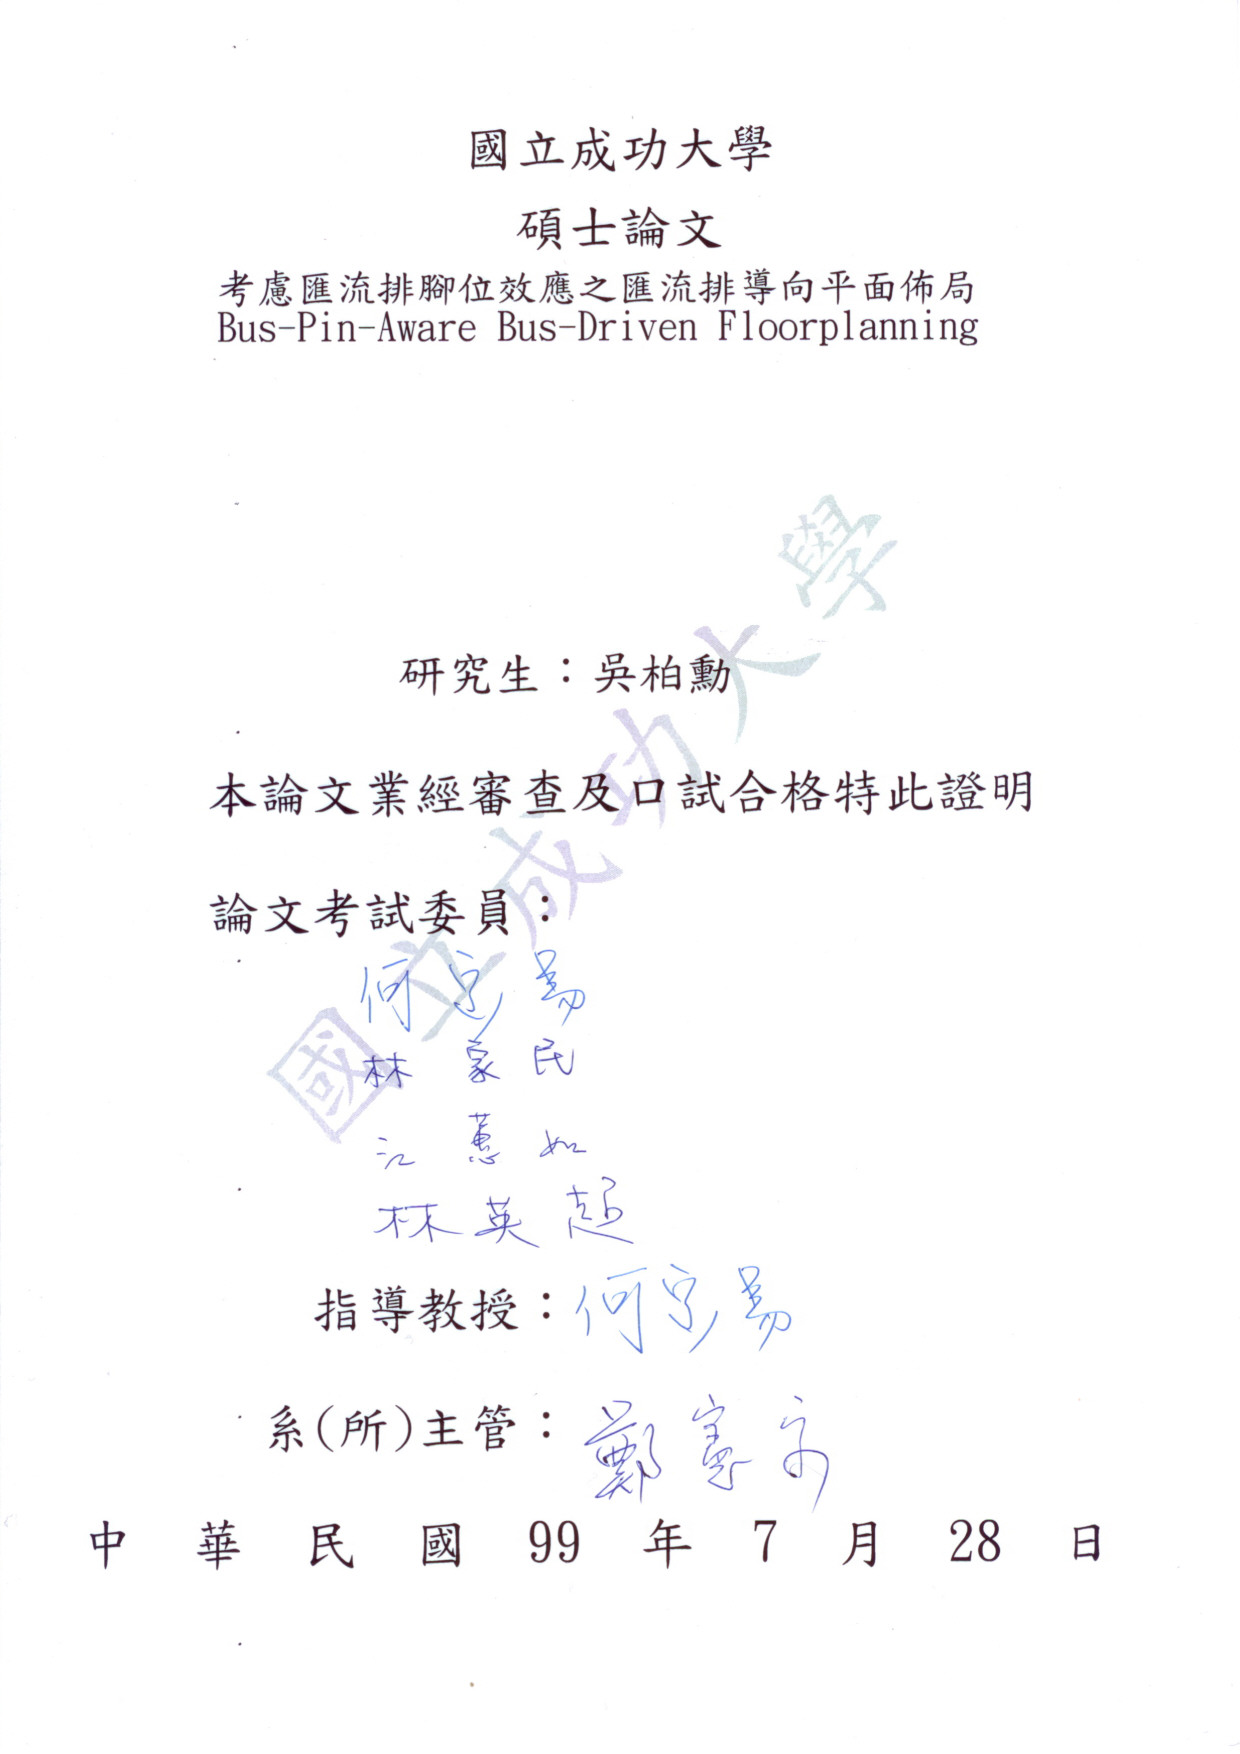
\includegraphics[]{./ncku/oral-chi.pdf}
\end{tabular}
\end{figure}
\newpage
\newpage

\begin{figure}[h]
\centering
\vspace{-29mm}
\begin{tabular}{c}
\hspace{-36mm} 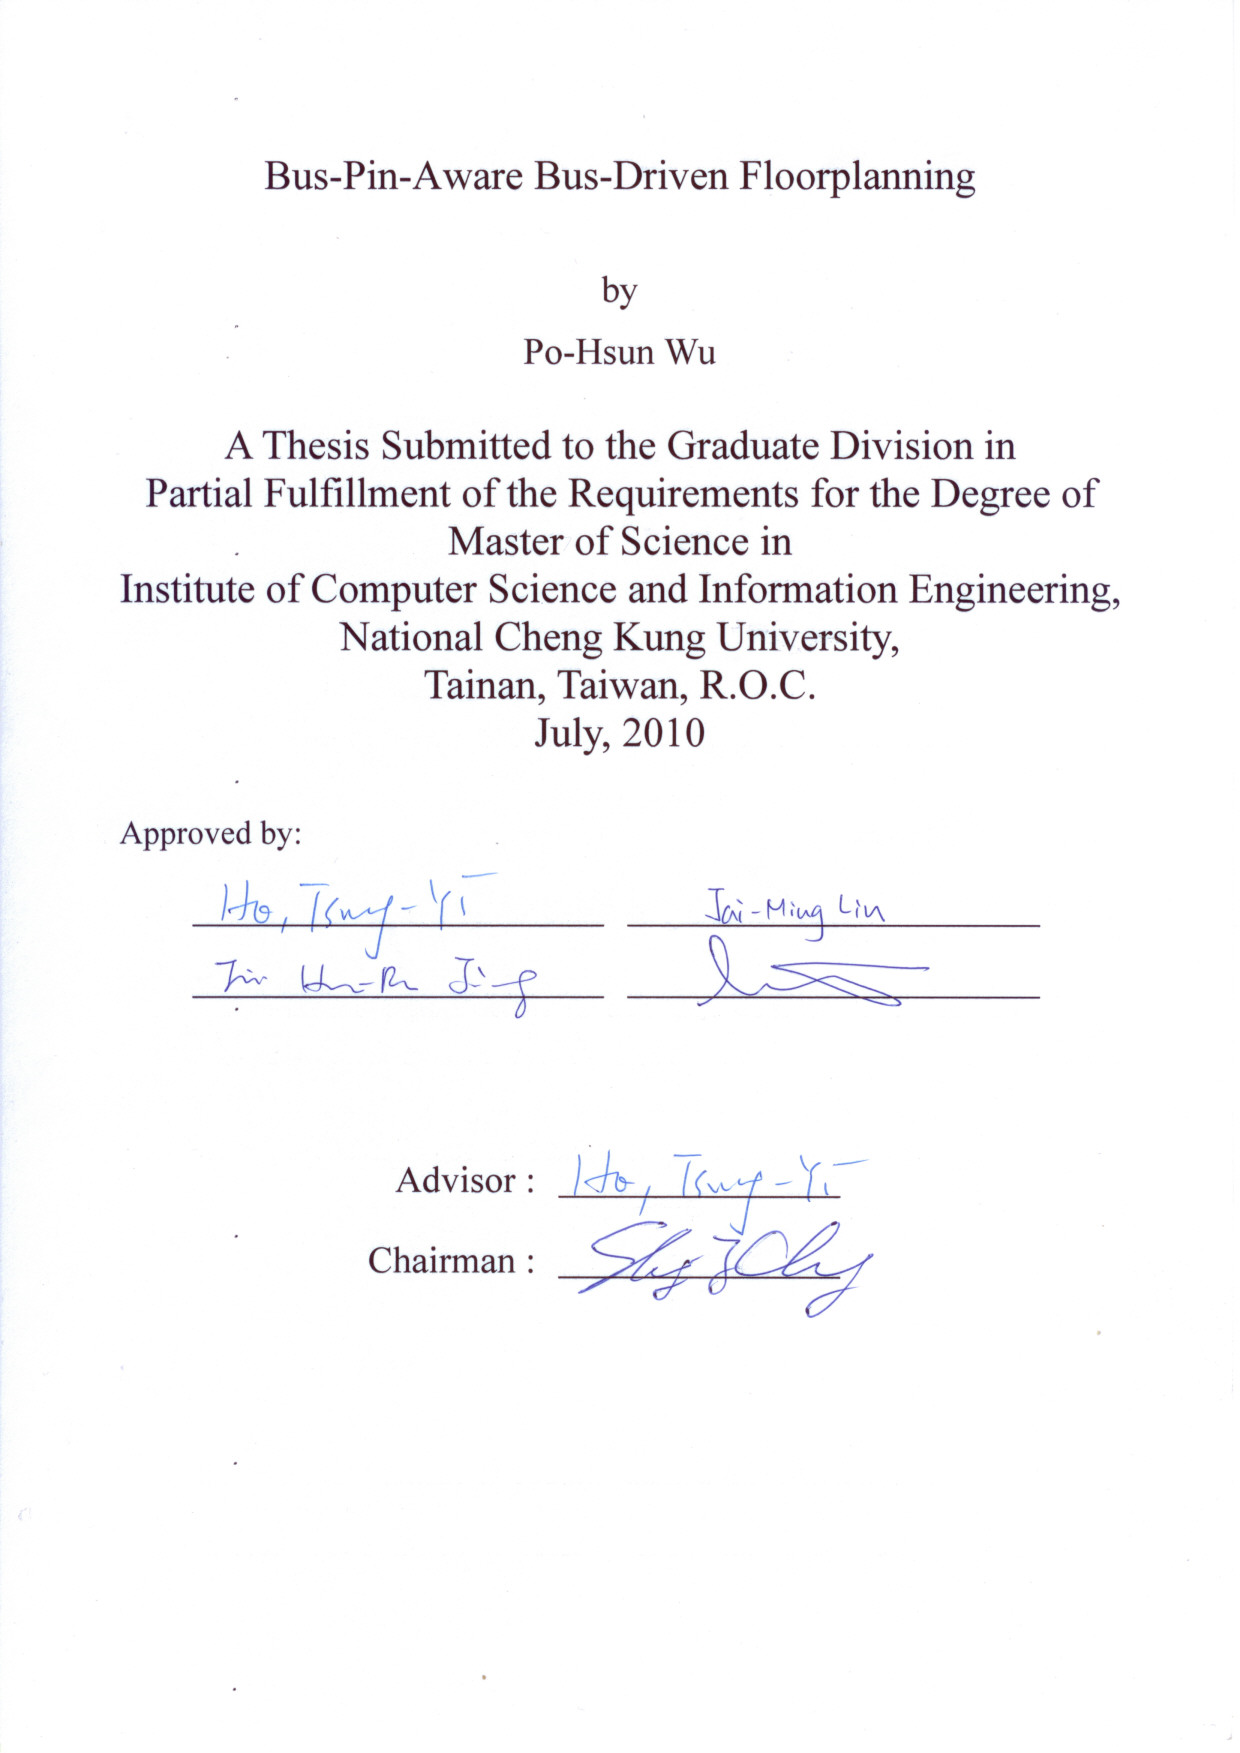
\includegraphics[]{./ncku/oral-eng.pdf}
\end{tabular}
\end{figure}
\newpage
\newpage

%
% Place your Chinese abstract here. The abstract heading will be
% generated automatically.
% Note: do NOT use \begin{abstract} ... \end{abstract}
%
\begin{figure}[h]
\centering
\vspace{-29mm}
\begin{tabular}{c}
\hspace{-36mm} 
\includegraphics[]{./abstract/ChineseAbstract1.pdf}
\end{tabular}
\end{figure}
\newpage
\newpage

\begin{figure}[h]
\centering
\vspace{-29mm}
\begin{tabular}{c}
\hspace{-36mm} 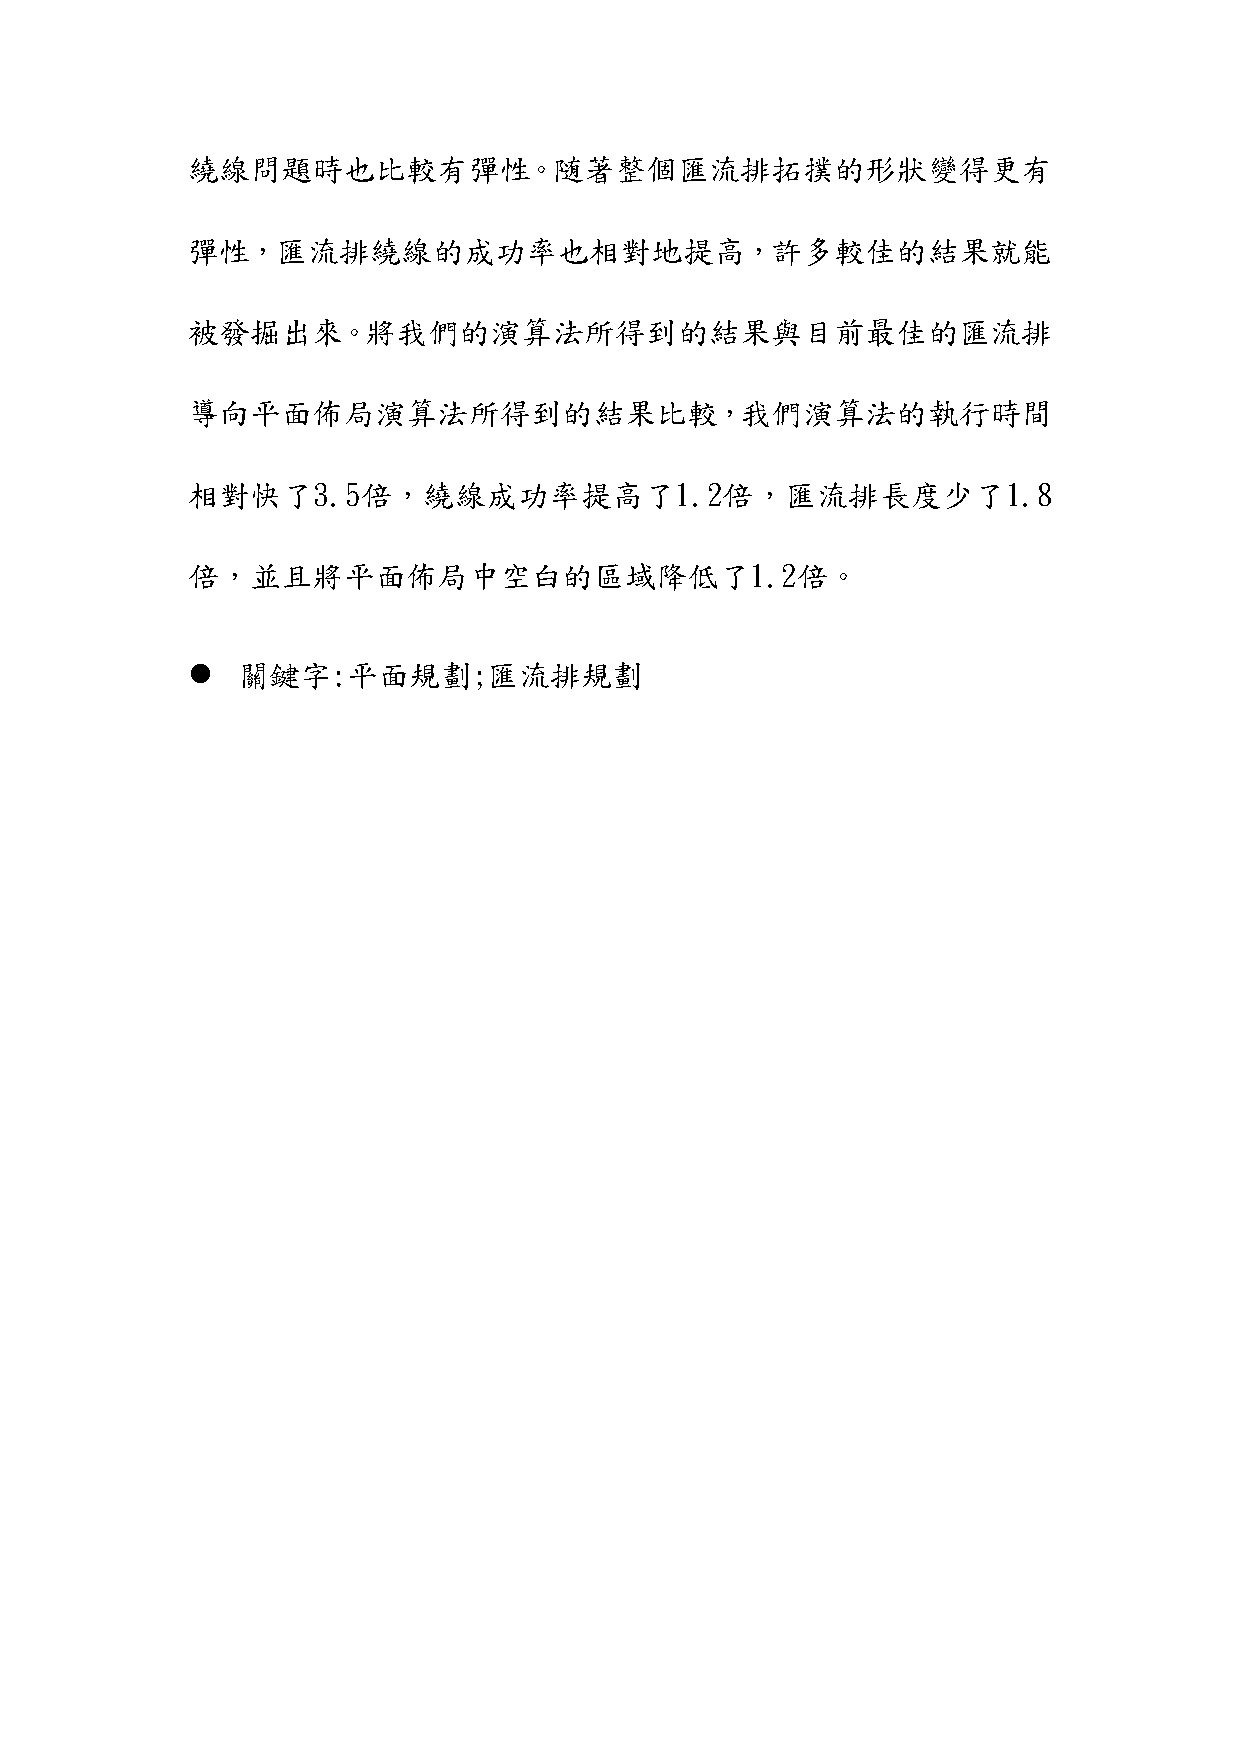
\includegraphics[]{./abstract/ChineseAbstract2.pdf}
\end{tabular}
\end{figure}
\newpage
\newpage

%% 從摘要到本文之前的部份以小寫羅馬數字印頁碼
% 但是從「書名頁」(但不印頁碼) 就開始計算
\setcounter{page}{1}
\pagenumbering{roman}

%
% Place your English abstract here. The abstract heading will be
% generated automatically.
% Note: do NOT use \begin{abstract} ... \end{abstract}
%
\begin{center}
\large \textbf{Bus-Pin-Aware Bus-Driven Floorplanning} \\[15mm]
\normalsize \textbf{Student: Po-Hsun Wu \hspace{5mm} Advisor: Dr. Tsung-Yi Ho\\[7mm]}
\normalsize \textbf{Department of Computer Science and\\
                    Information Engineering \\
                    National Cheng Kung University\\
                    Tainan, Taiwan, R.O.C.\\[7mm]}
\large \textbf{Abstract}
\end{center}
%%%%%%%%%%%%%%%%%%%%%%%%%%
\label{abs}
%%%%%%%%%%%%%%%%%%%%%%%%%%

\baselineskip=26pt


As the number of buses increase substantially in multi-core SoC
designs, the bus planning problem has become the dominant factor
in determining the performance and power consumption of SoC
designs. To cope with the bus planning problem, it is desirable to
consider this issue in early floorplanning stage. Recently,
bus-driven floorplanning problem has attracted much attention in
the literature. However, current algorithms adopt an
over-simplified formulation ignoring the position and
orientation of the bus pins, the chip performance may be deteriorated.
In this paper, we propose the bus-driven
floorplanning algorithm that fully considers the impacts of the bus
pins. By fully utilizing the position and orientation of the bus pins,
bus bendings are not restricted to occur at the modules on the bus,
then it has more flexibility during bus routing. With more
flexibility on the bus shape, the size of the solution
space is increased and a better bus-driven floorplanning solution
can be obtained. Compared with the bus-driven
floorplanner \cite{Ma08}, the experimental results show that our
algorithm performs better in runtime by 3.5$\times$, success rate
by 1.2$\times$, wirelength by 1.8$\times$, and reduced the
deadspace by 1.2$\times$.


\begin{itemize}
\item {\bf Keywords:} Floorplanning; Bus planning

\end{itemize}
               % English Abstract

%\specialspacing
%acknowledgements
%
% Place the text of your acknowledgments here. Your name and
% graduation date will appear automatically. If this is the preface
% instead of acknowledgments, use \preface.
% Note: do NOT use \begin{acknowledgements} ... \end{acknowledgements}
%
%%\input{abs/ackno}
%\doublespacing

%
% ----------------------------------------------------------------------------
%                            English acknowledgments
%                                   英文致謝
% ----------------------------------------------------------------------------

% Set the line spacing
\baselineskip = 26pt

% ------------------------------------------------

% Page start
\newpage
\phantomsection

% Add to "Table of Contents"
\addcontentsline{toc}{chapter}{Acknowledgments}

% ------------------------------------------------

\begin{center}
\large \textbf{Acknowledgments}
%\label{acknowledgments}
\end{center}

% ------------------------------------------------

"我思故我在, 我做故我存."\\
"I think, therefore I am. I do, that become valuable."\\

"別人笑我太瘋癲,我笑他人看不穿."\\
"People laugh at me for my insane, but I laugh them because they don't see the truth."\\

% ------------------------------------------------

% End of page

% ------------------------------------------------




\setcounter{secnumdepth}{10}
\tableofcontents    % Table of Contents will be automatically
                    % generated and placed here.

\listoftables       % List of Tables and List of Figures will be placed
\listoffigures      % here, if applicable.

\newpage

%%%%%%%%%%%%%%%%%%%%%%%%%%%
% Actual text starts here %
%%%%%%%%%%%%%%%%%%%%%%%%%%%

%\onehalfspacing

%%%%%%%%%%%%%%%%%%%%%%%%%%
\chapter{Introduction}
\label{chap::intro}
%%%%%%%%%%%%%%%%%%%%%%%%%%

\baselineskip=26pt

\thispagestyle{empty}

\hspace{5mm}With the increasing design
complexity, the amount of buses between different modules on a
chip also increases rapidly. Bus routing has become a major
concern of comparable importance to timing and power in multi-core
SoC designs. To ease the efforts of bus routing in later routing
stage, it is desirable to consider this issue in early floorplanning
stage. Since buses are of different widths and required to go
through different sets of modules, the bus routability
is severely affected by the module position. Bus-driven
floorplanning targets on obtaining a bus-routable floorplan such
that the chip area and the bus area are
minimized. Recently, many bus-driven floorplanning algorithms have
been proposed in the literature \cite {Rafiq02, Xiang03, Chen05,
Law05, Xiang07, Ma08, Kim08_1, Kim08_2, Sheng10, He10, PH10}.
However, these bus-driven floorplanning algorithms
adopt an over-simplified formulation which ignores the practical
issues such as the position and orientation of the bus pin.
Without taking those practical issues into consideration,
it may have the following impacts on bus routing:
\begin{itemize}
\item \textbf{Bus twisting:} It makes the signal wires cross at a
point and decreases accessibilities of the bused pins.
\item \textbf{Via increasing:}
Several vias occur at the bend of a bus that have adverse effects
on the bus delay.
\item \textbf{Delay variation:} Different
driver-load wirelength between different bus bits causes
delay variation among all bus bits.
\end{itemize}

\begin{figure}[htb]
  \centering
    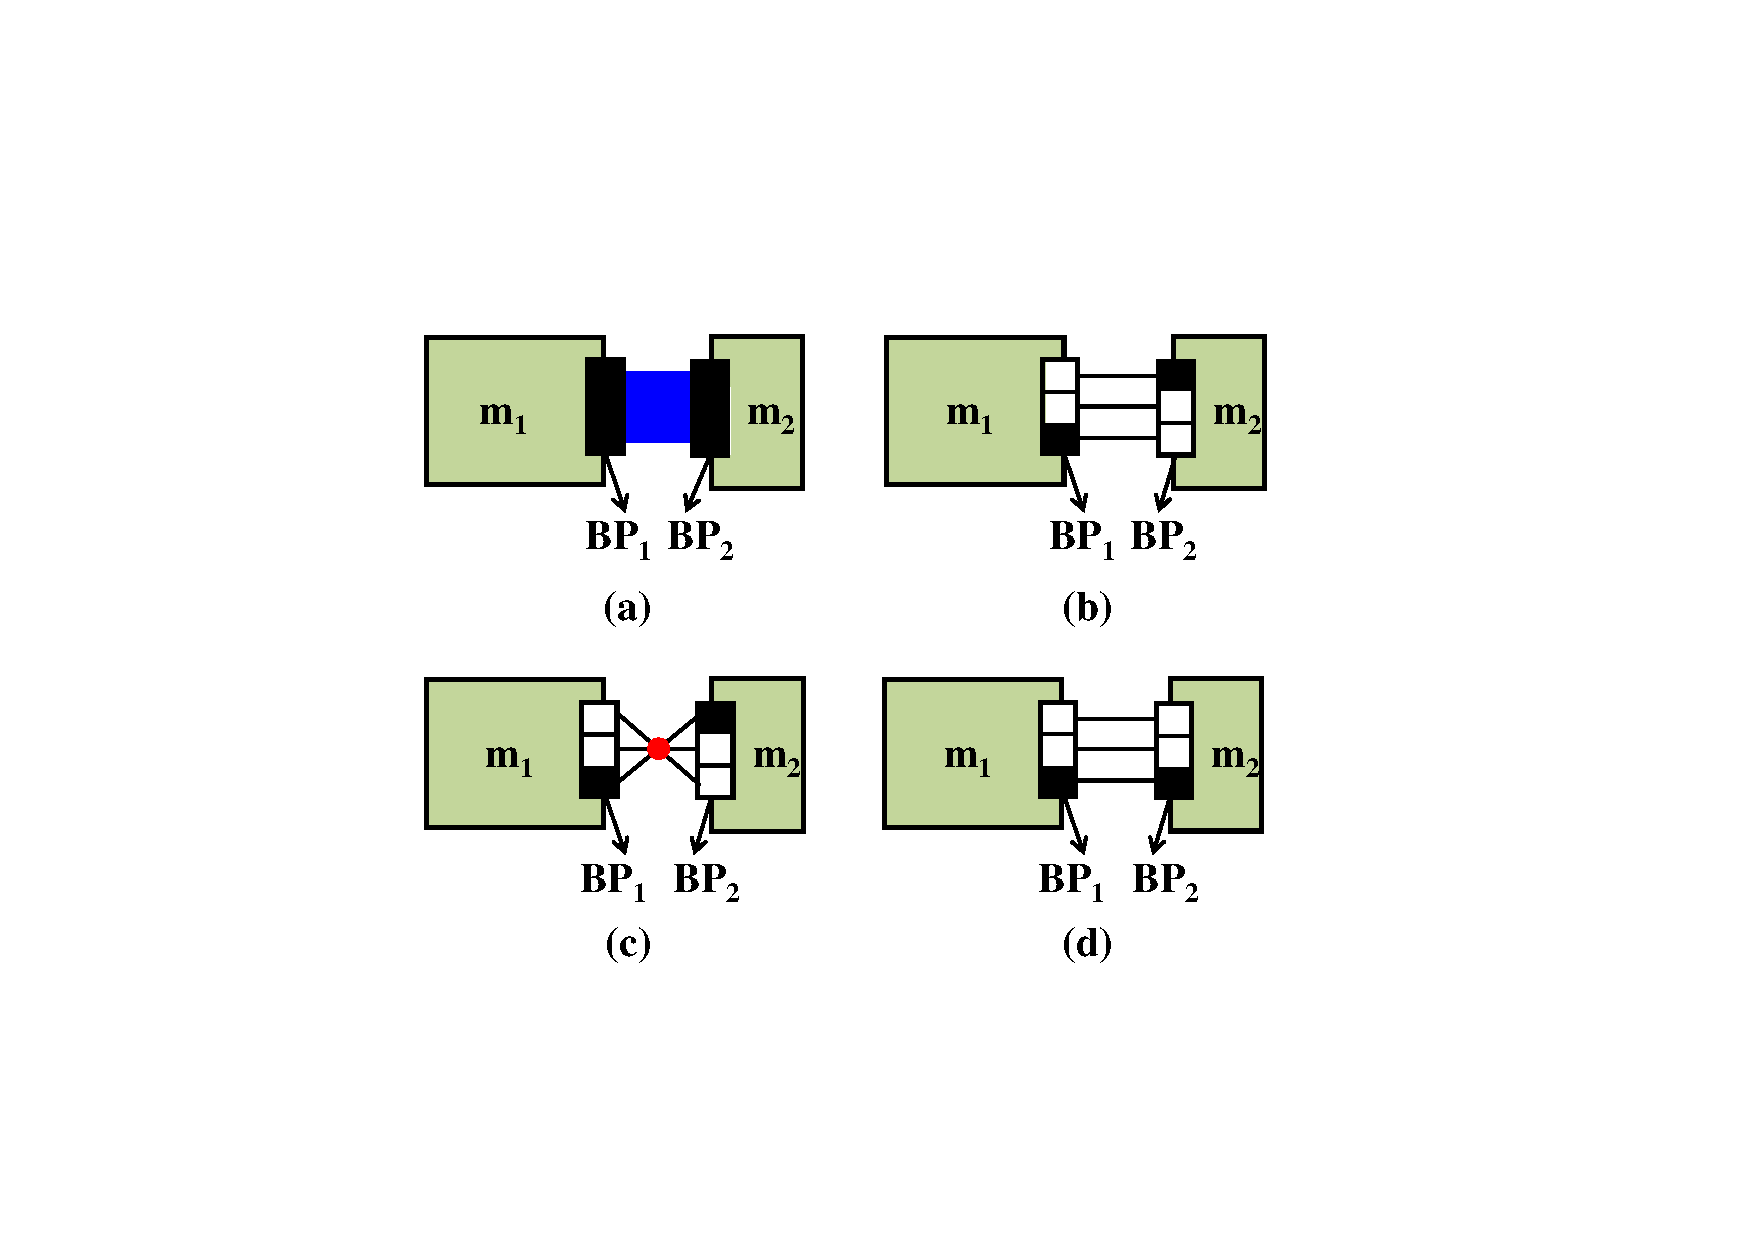
\includegraphics[width=8.8cm]{Fig/bus_twisting.pdf}
    %\centerline{\psfig{figure=Fig/bus_twisting.eps, width=8.8cm}}
     \caption{
      (a) One horizontal bus connects two bus pins. (b) Bus routing without considering the effect of the bus pin. (c) Bus twisting. (d) No bus twisting after flipping the bus pin.
   }
  \label{fig::bus_twisting}
\end{figure}

One example of the bus twisting is given in Figure~\ref{fig::bus_twisting}.
In Figure~\ref{fig::bus_twisting} (a), two modules $m_1$ and $m_2$ are placed
on the floorplan, and two bus pin $BP_1$ and $BP_2$ connected by one horizontal bus
are placed on the boundary of the two modules. Since the effect of the bus pin
is not considered during bus routing in current algorithms,
the routing result in Figure~\ref{fig::bus_twisting} (b)
is obtained, and some bits of the bus pin are not correctly connected
by the wire. Therefore, the wrong signal is transmitted via the bus,
the Most Significant Bit (MSB) of each bus pin is marked with black color
in all figures of this paper.
In this paper, the bus pin is carefully handled during bus routing, thus,
each bus can be correctly connected by the wire as shown in Figure~\ref{fig::bus_twisting} (c).
However, all wires are twisted at one point in the figure,
the problem can be solved by flipping the bus pin $BP_2$ as shown in Figure~\ref{fig::bus_twisting} (d).

Therefore, an over-simplified bus-driven floorplanning formulation will
make the routability and the solution quality in doubt.

\begin{figure}[htb]
  \centering
    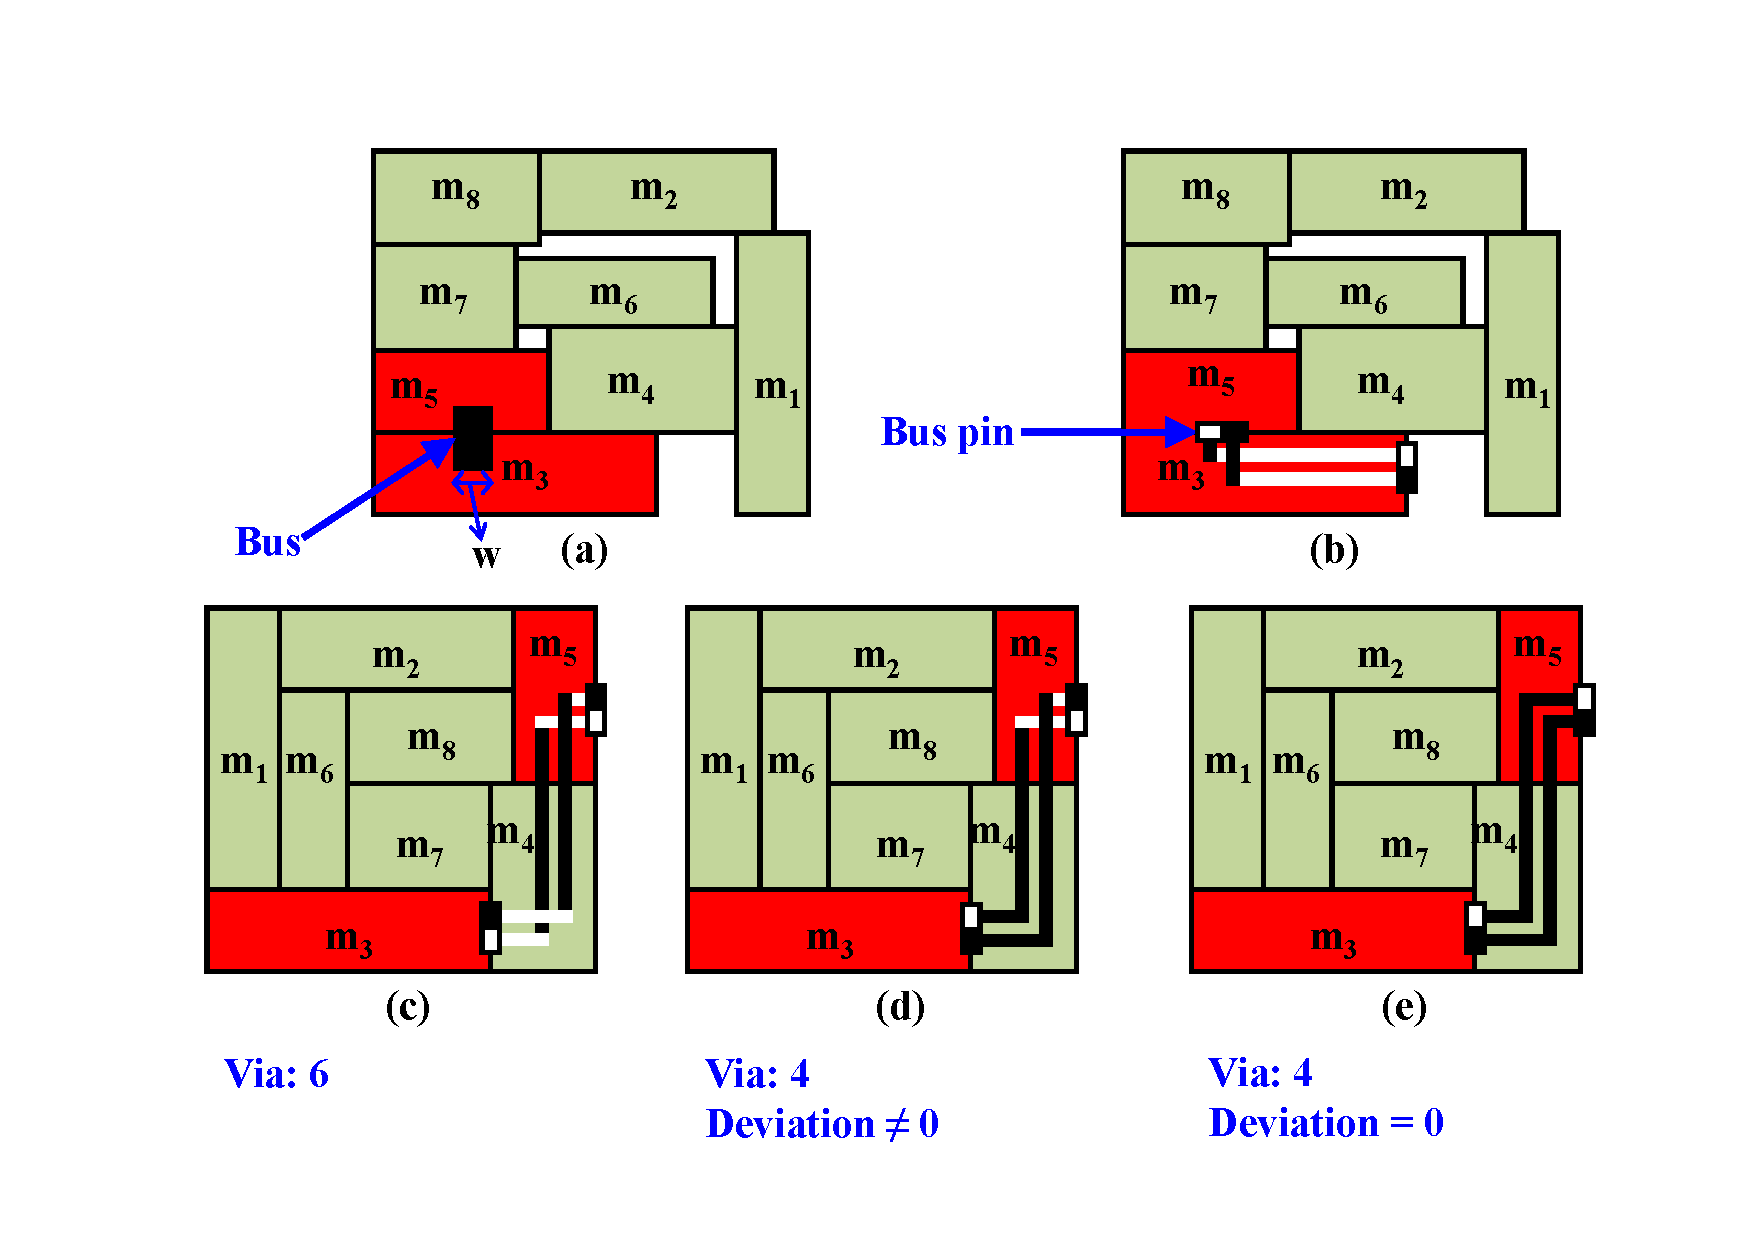
\includegraphics[width=13cm]{Fig/introduction_example.pdf}
    %\centerline{\psfig{figure=Fig/introduction_example.eps, width=13cm}}
     \caption{
      (a) Simplified bus routing. (b) Bus routing considering the bus pin. (c) Bus routing with the diagonal connection between the modules. (d) Via-aware bus routing with the diagonal connection between modules. (e) Bus routing considering both vias and wirelength deviation.
   }
  \label{fig::introduction_example}
\end{figure}

Figure~\ref{fig::introduction_example} illustrates the impact of
the position and orientation of the bus pin. There are eight
modules and one bus that connects two modules $m_3$ and $m_5$,
i.e., bus modules. In Figure~\ref{fig::introduction_example} (a),
existing bus-driven floorplanning algorithms connect $m_3$ and
$m_5$ by simply one vertical bus. However, by considering the
actual positions of the bus pins in
Figure~\ref{fig::introduction_example} (b), the bus pins of these
two modules can not be passed by only one vertical bus, and the
wirelength is much longer than the simplified estimation.

Furthermore, current bus-driven floorplanning algorithms restrict
a bus only bends above the bus modules, i.e., only
horizontal and vertical connections on the bus modules are
allowed. Such restriction limits the flexibility on the bus shape
resulting a narrower solution space. Therefore,
better bus-driven floorplanning solutions may be missed in such
formulation. In this paper, we explore the diagonal connection
between the bus modules to improve the solution quality. Compared with
Figure~\ref{fig::introduction_example} (b), a better solution with
smaller area can be achieved by utilizing the diagonal connection
between $m_3$ and $m_5$ as shown in
Figure~\ref{fig::introduction_example} (c). Although there are two
bends occur at two modules $m_4$ and $m_5$,
no extra vias are required at the bend of $m_5$ since vias exist
anyway to connect to the bus modules $m_5$. Even extra vias are
still required at another bend on the module $m_4$ which is not
a bus module, it can be eliminated by simply flipping the bus
pin on the module $m_3$ and assigning the horizontal and vertical
buses on the module $m_4$ to the same layer as shown in
Figure~\ref{fig::introduction_example} (d).

As mentioned earlier, different driver-load wirelength between bus
bits causes delay variation among all bus bits. At a load,
the wirelength difference among all bus bits is characterized by
\textbf{wirelength deviation}. Different from
Figure~\ref{fig::introduction_example} (d), the driver-load
bus delay among all bus bits is different, the deviation can be
further optimized to 0 by flipping the bus pin on module $m_5$ as
shown in Figure~\ref{fig::introduction_example} (e).

In this paper, we propose a bus-driven
floorplanning algorithm that fully considers the impact of the
bus pins. By fully utilizing the position and orientation of the
bus pins, we can obtain the high-quality results by exploring
flexibility on the bus shape. Moreover, we also
develop two effective algorithms to minimize the wirelength
deviations and two wirelength reduction algorithms to optimize
the total bus wirelength. Experimental results show that our
algorithms are very promising.

\section{Previous Works}
\label{sec::Previous Works}
The bus-driven floorplanning problem has recently attracted a lot of
attention in the literature. Rafiq et al. proposed an integrated
floorplanning for bus-based microprocessor designs \cite{Rafiq02}.
Multiple topologies were produced for each bus, and a mixed
integer/linear programming approach was adopted to arbitrate the
conflicts between different buses. However, the algorithm was limited to
single fanout buses. Xiang et al. \cite{Xiang03}
solved the bus-driven floorplanning problem by using a
sequence pair (SP) representation based on a simulated annealing (SA)
framework. Chen and Chang \cite{Chen05} handled the bus-driven
floorplanning problem based on the B*-tree representation. The
drawback of the above two methods is that all modules are
connected by either horizontal or vertical 0-bend buses; the
solution space is thus restricted when a large number of the modules
are involved for each bus.
The bus shape problem was improved by \cite{Law05}, where
0-bend, 1-bend, and 2-bend buses were allowed. Nevertheless, there are still
limitations on the bus shape. In \cite{Ma08}, a
multi-bend bus-driven floorplanning algorithm was proposed based on
a TCG representation. It has more flexibility on bus shapes and
obtains higher success rate.

In microprocessors and DSPs, many cores are involved and the signals
are transmitted between different cores by the buses which
play an important role in determining the chip performance.
Therefore, some previous works were developed to deal with
such floorplanning in microarchitectural design.
Kim and Lim \cite{Kim08_1} presented a new bus routing algorithm
based on Hanan grids and linear programming. In \cite{Kim08_2},
the authors proposed a bus-aware microarchitectural floorplanning
which addressed the impact of bus routability on performance/power/thermal issues.
However, the above two works aimed on optimizing IPC (Instructions Per Cycle) and
had a different problem formulation from those aforementioned
floorplanners.

There are still many works which consider other constraints during the bus planning.
Xiang et al. \cite{Xiang07} proposed an OPC-friendly bus driven
floorplanning algorithm which carefully designed the pitch
for buses to avoid the forbidden pitch.
Sheng et al. \cite{Sheng10} proposed an approach which was based on a deterministic
algorithm Less Flexibility First, it run in a fixed-outline area and packed hard blocks one after another.
In \cite{He10}, they presented a floorplan revising method which was based on linear
programming model to minimize the number of reducible routing vias with a controllable
loss on the chip area and wirelength.
The authors \cite{PH10} considered the bus pin issue and explored the diagonal connection
which makes the bus shape more flexible and improves the solution quality.

\section{Our Contributions}
\label{sec::Our Contributions}
%bus-driven
In this paper, we propose a bus-driven
floorplanning algorithm that fully considers the impact of the
bus pins. The diagonal connection between
different modules is explored to make the bus shape more flexible which improves
the success rate.
The contributions of this paper are listed as follows:\\
\begin{itemize}
\item \textbf{Deviation Minimization:}
%deviation
We develop two algorithms to
minimize the wirelength deviation for signal integrity of the buses.
First algorithm explores all possible topologies between any two modules,
and it finally concludes some specific bus patterns,
then the best deviation at each module can be quickly obtained from
those specific bus patterns.
In second algorithm, the procedure of determining the deviation at
each module is divided into two steps --- deviation determination and
accumulated deviation update.
During determining the deviation at one module, all the accumulated deviation
from the driver to its neighbors can also be calculated.
Since the procedure of determining the deviation at each module
is divided into two steps, the segment size for each comparison
becomes smaller, then the total bus patterns can be further reduced to 10 types.
Fewer bus patterns stands for less time is needed for searching the possible bus patterns.
Experimental results show that the wirelength deviation can be effectively reduced.

\item \textbf{Diagonal relation:}
%success rate
In this paper, we explore the diagonal relation between different
modules to make the bus shape more flexible, then the modified
graph coloring algorithm is proposed to determine the layer of each
bus. Experimental results show that our algorithm has
1.2$\times$ improvement on the success rate compared with
\cite{Ma08}.

\item \textbf{Wirelength reduction:}
%wirelength reduction
To further enhance the solution quality, we present two wirelength
reduction algorithms to improve the total bus wirelength.
First algorithm reduces the total bus wirelength by minimizing the
overlap between different bus components
(for the multi-bend bus, each horizontal (vertical) part is called a bus component)
during constructing the minimum spanning tree (MST).
The second algorithm is used to optimize the bus wirelength by
adjusting the coordinate of each horizontal (vertical) bus component.
\end{itemize}

The rest of this paper is organized as follows.
Chapter~\ref{chap::PROBLEM FORMULATION} gives the problem
formulation of the bus-driven floorplanning.
%
Chapter~\ref{chap::CONSTRAINTS AND TERMINOLOGIES} defines the
constraints and terminologies used in this paper.
%
Chapter~\ref{chap::ALGORITHM} gives the details of the proposed
bus-driven floorplanning algorithm.
%
Experimental results are shown in
Chapter~\ref{chap::EXPERIMENTAL RESULTS}.
%
Finally, a conclusion will be given in
Chapter~\ref{chap::CONCLUSIONS}.

\vfill\eject

\thispagestyle{empty}
\newpage

%%%%%%%%%%%%%%%%%%%%%%%%%%
\chapter{Problem Formulation}
\label{chap::PROBLEM FORMULATION}
%%%%%%%%%%%%%%%%%%%%%%%%%%

\baselineskip=26pt

\hspace{5mm}Since long or timing
critical buses are normally assigned to a pair of high metal
layers, one horizontal and one vertical, we only consider the
two-layer bus routing problem. The horizontal and vertical buses
can be routed in either layer. In the bus-pin-aware bus-driven
floorplanning problem, we are given the following:

1. A set of $n$ modules $M =$ \{$m_1$, $m_2,..., m_n$\}, each module $m_i$
is associated with height $h_i$ and width $w_i$, where $h_i, w_i \in$
$R^+$.

2. A set of $m$ buses $B =$ \{$b_1$, $b_2,..., b_m$\}, each bus $b_j$ has a
width $t_j$ and goes through a set of modules. Moreover, the
position of each bus pin is also defined in each bus, where
$t_j \in R^+$.

Our goal is to determine the orientation and position of the bus pins
on each module and decide the routing path for each bus such
that no overlapping occurs between different horizontal (vertical)
bus components.
Moreover, no overlapping is allowed between different modules.
The objectives of the bus-pin-aware bus-driven floorplanning problem are:\\
(1) to {\bf minimize the chip area},\\
(2) to {\bf minimize the bus area},\\
(3) to {\bf minimize the number of infeasible buses},\\
(4) to {\bf minimize the deviation of each bus}.\\

%%%%%%%%%%%%%%%%%%%%%%%%%%
\chapter{Constraints and Terminologies}
\label{chap::CONSTRAINTS AND TERMINOLOGIES}
%%%%%%%%%%%%%%%%%%%%%%%%%%

\baselineskip=26pt
\hspace{5mm}
In this section, the capacity constraint in bus-pin-aware bus-driven floorplanning
are defined, followed by the introduction of the terminologies
used in this paper.

\begin{figure}[htb]
  \centering
    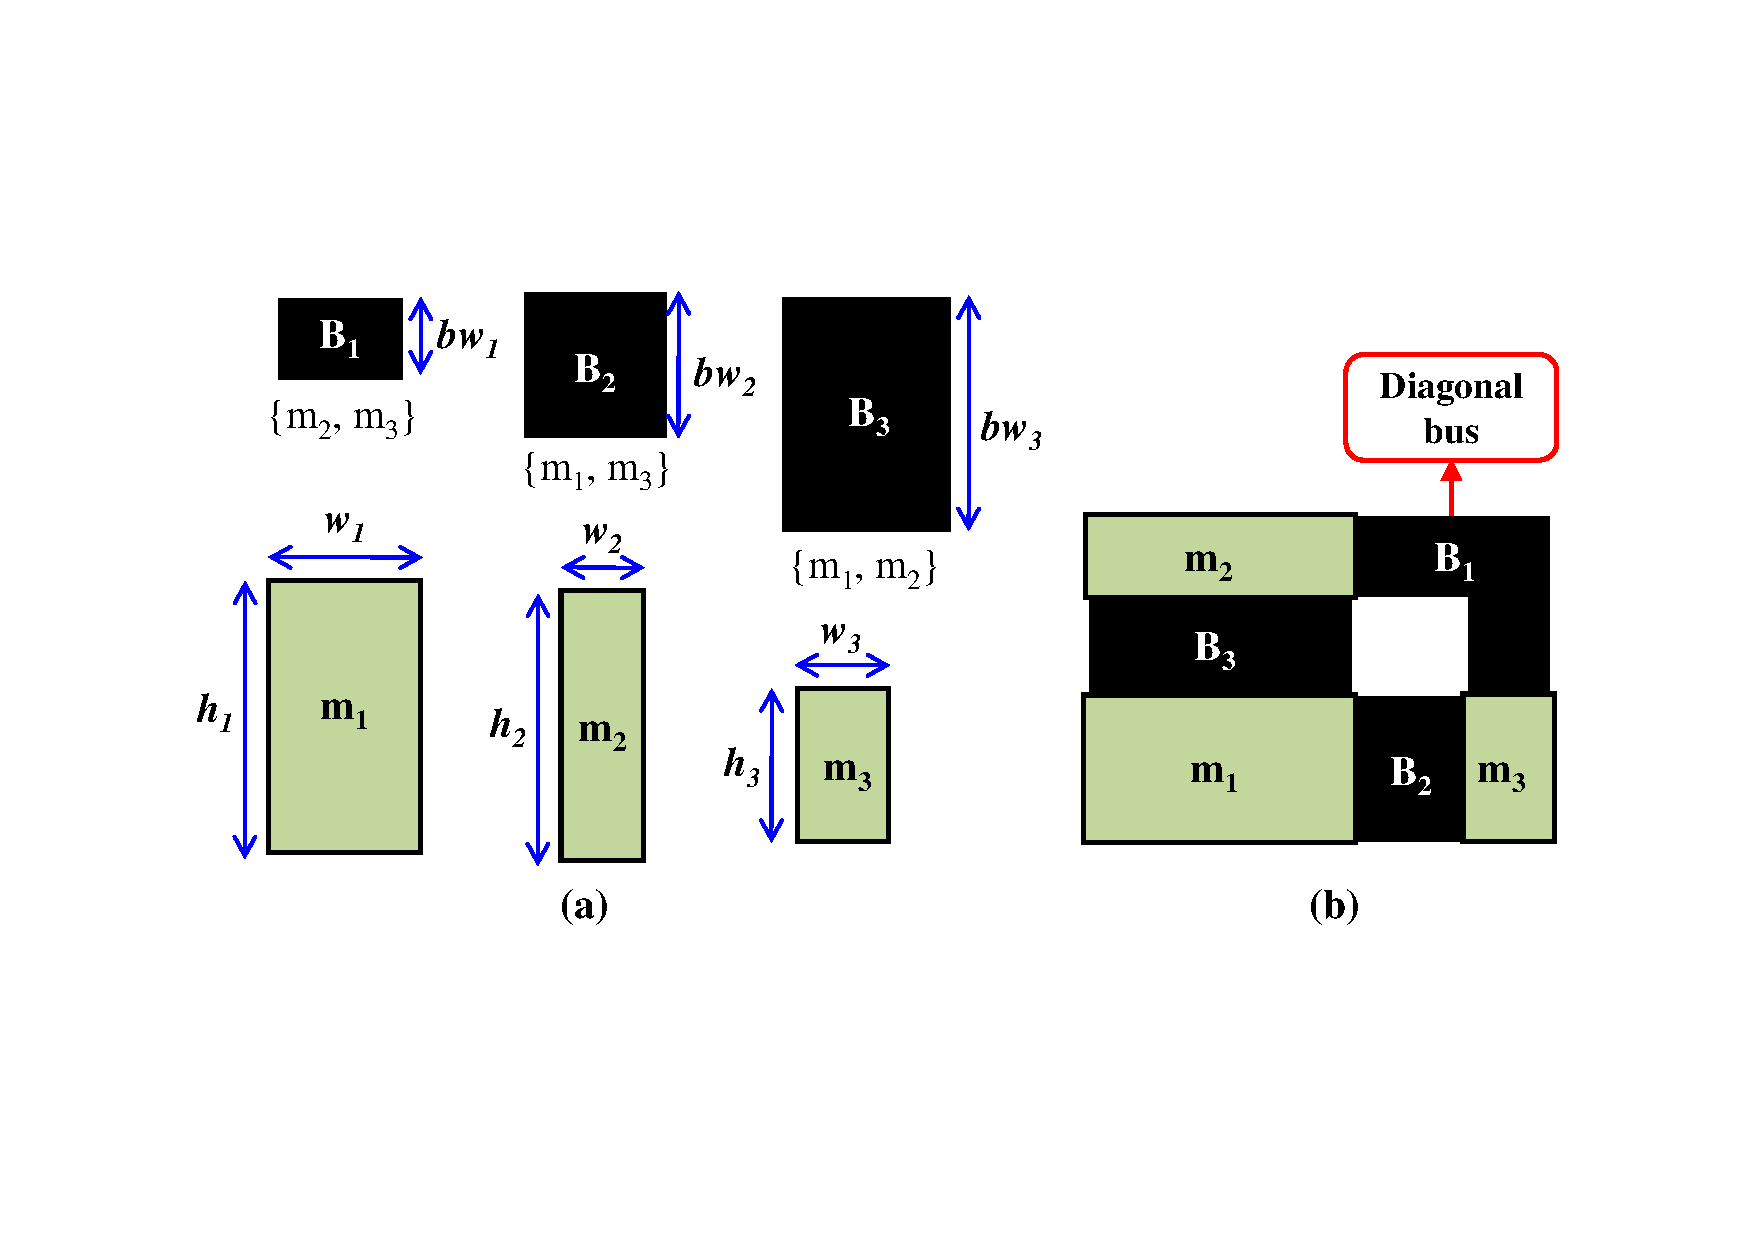
\includegraphics[width=12cm]{Fig/capacity.pdf}
    %\centerline{\psfig{figure=Fig/capacity.eps, width=12cm}}
  \caption{
      (a) Capacity constraint. (b) A routable solution under the capacity
      constraint.
   }
  \label{fig::capacity}
\end{figure}

Capacity constraint is illustrated in Figure~\ref{fig::capacity}
(a). There are three buses $B_1$ = \{$m_2$, $m_3$\}, $B_2$ = \{$m_1$, $m_3$\}, and
$B_3$ = \{$m_1$, $m_2$\}, moreover, three modules $m_1$, $m_2$, and $m_3$ are
placed on the floorplan. $bw_i$ is the bus width of bus
$B_i$, and the width and height of each module $m_i$ are
denoted by $w_i$ and $h_i$, respectively.

Since the capacity of each module is limit, some modules can be passed with only
one bus at the same direction. For instance, $bw_2$ + $bw_3 >$
max($w_1$, $h_1$), therefore, the capacity of the module $m_1$ is
not enough for both buses $B_2$ and $B_3$ to pass through.

Compared with existing bus-driven floorplanning algorithms which
result in an unroutable solution in this example, we can have a
routable solution by exploring the diagonal connection between
different modules in Figure~\ref{fig::capacity} (b). The modified
graph coloring algorithm is proposed to assign the bus components
of the diagonal bus $B_1$ to the same layer such that no extra via
is required at the bend of the bus $B_1$.

\begin{figure}[htb]
  \centering
    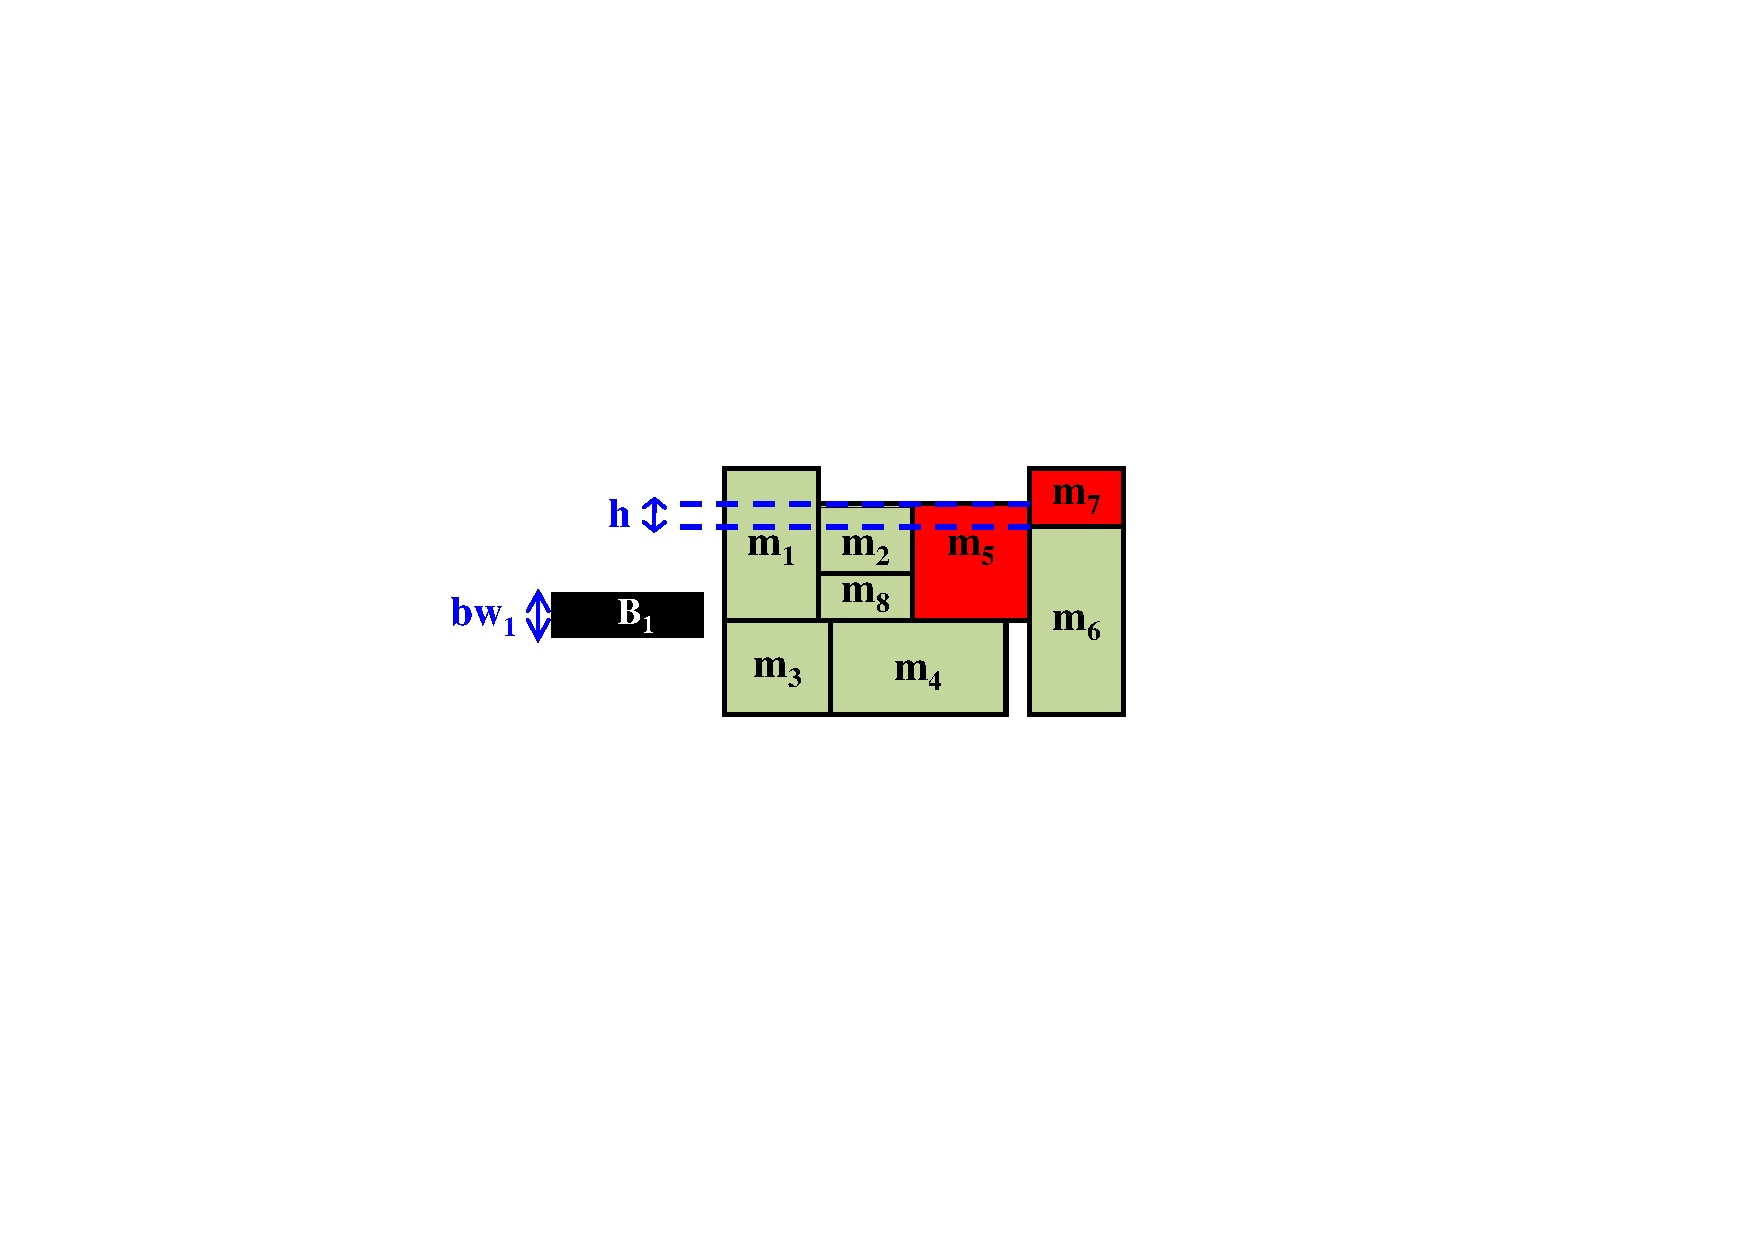
\includegraphics[width=7cm]{Fig/vertical_overlapping.pdf}
    %\centerline{\psfig{figure=Fig/vertical_overlapping.eps, width=7cm}}
     \caption{
      Vertical overlapping.
   }
  \label{fig::vertical_overlapping}
\end{figure}

Another constraint is vertical overlapping as shown in
Figure~\ref{fig::vertical_overlapping}, the bus width of $B_1$
is $bw_1$ and it connects two modules $m_5$ and $m_7$, the
overlapped range between two modules is $h$. If $h < bw_1$, then
it has no sufficient space for the bus $B_1$ to pass through that
the vertical overlapping constraint is violated, thus, the coordinate
of the module $m_5$ must be adjusted to increase the overlapped range.

Terminologies used in this paper are introduced as follows:

{\bf Definition 1}: A \textbf{\textit{bus pin}} of an n-bit bus
consists of n pins. The bits of each bus pin are arranged
monotonically from the Least Significant Bit (LSB) to the MSB,
and are equally spaced. The MSB bit is marked with black color
in all figures of this paper. A bus pin is
oriented horizontally or vertically. For example, the bus pins
$BP_1$, $BP_2$, and $BP_6$ are oriented horizontally, and the bus
pins $BP_3$, $BP_4$, and $BP_5$ are oriented vertically in
Figure~\ref{fig::bus_pin_flipping} (a).

\begin{figure}[htb]
  \centering
    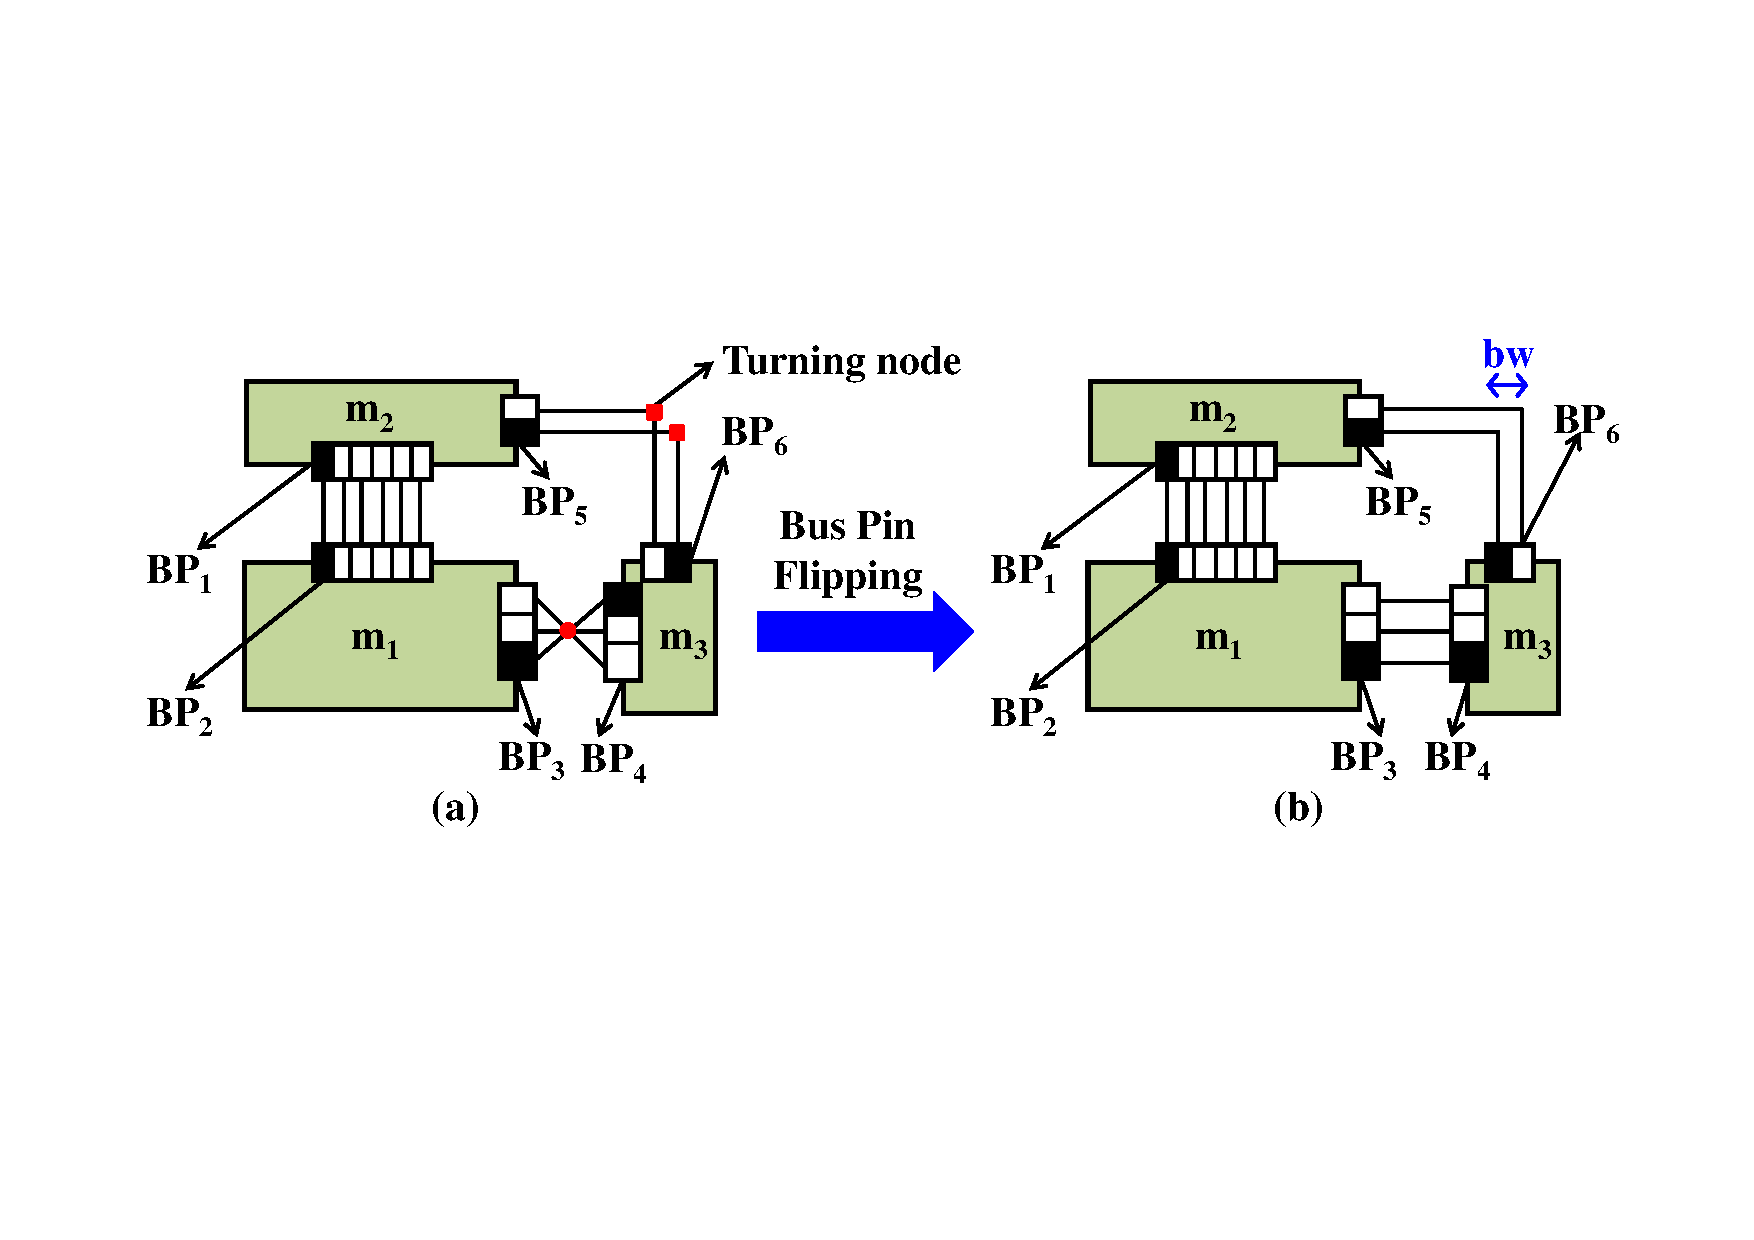
\includegraphics[width=13cm]{Fig/bus_pin_flipping.pdf}
    %\centerline{\psfig{figure=Fig/bus_pin_flipping.eps, width=13cm}}
     \caption{
      Bus pin flipping.
   }
  \label{fig::bus_pin_flipping}
\end{figure}

{\bf Definition 2}: The \textbf{\textit{position of the bus pin}}
is the position of the bus pin on the module, it can be placed on
one of the four boundaries of the modules. For example, the bus pin
$BP_1$ is placed on the lower boundary of the module $m_2$ in
Figure~\ref{fig::bus_pin_flipping} (a).

{\bf Definition 3}:  \textbf{\textit{Turning nodes}} denote the
bends of the buses and they are connected with the horizontal and
vertical buses. For example, there are two turning nodes at the
bend of the bus connecting the bus pins $BP_5$ and $BP_6$ in the
Figure~\ref{fig::bus_pin_flipping} (a).

{\bf Definition 4}: The \textbf{\textit{orientation of the bus
pin}} is defined as the direction from the LSB to the MSB. For
example, the orientation of the bus pin $BP_1$ is from east to west,
and the orientation of the bus pin $BP_3$ is from north to south in
Figure~\ref{fig::bus_pin_flipping}(a). All possible orientations
for the bus pins and the turning nodes are listed in
Figure~\ref{fig::orientation_direction}.

\begin{figure}[htb]
  \centering
    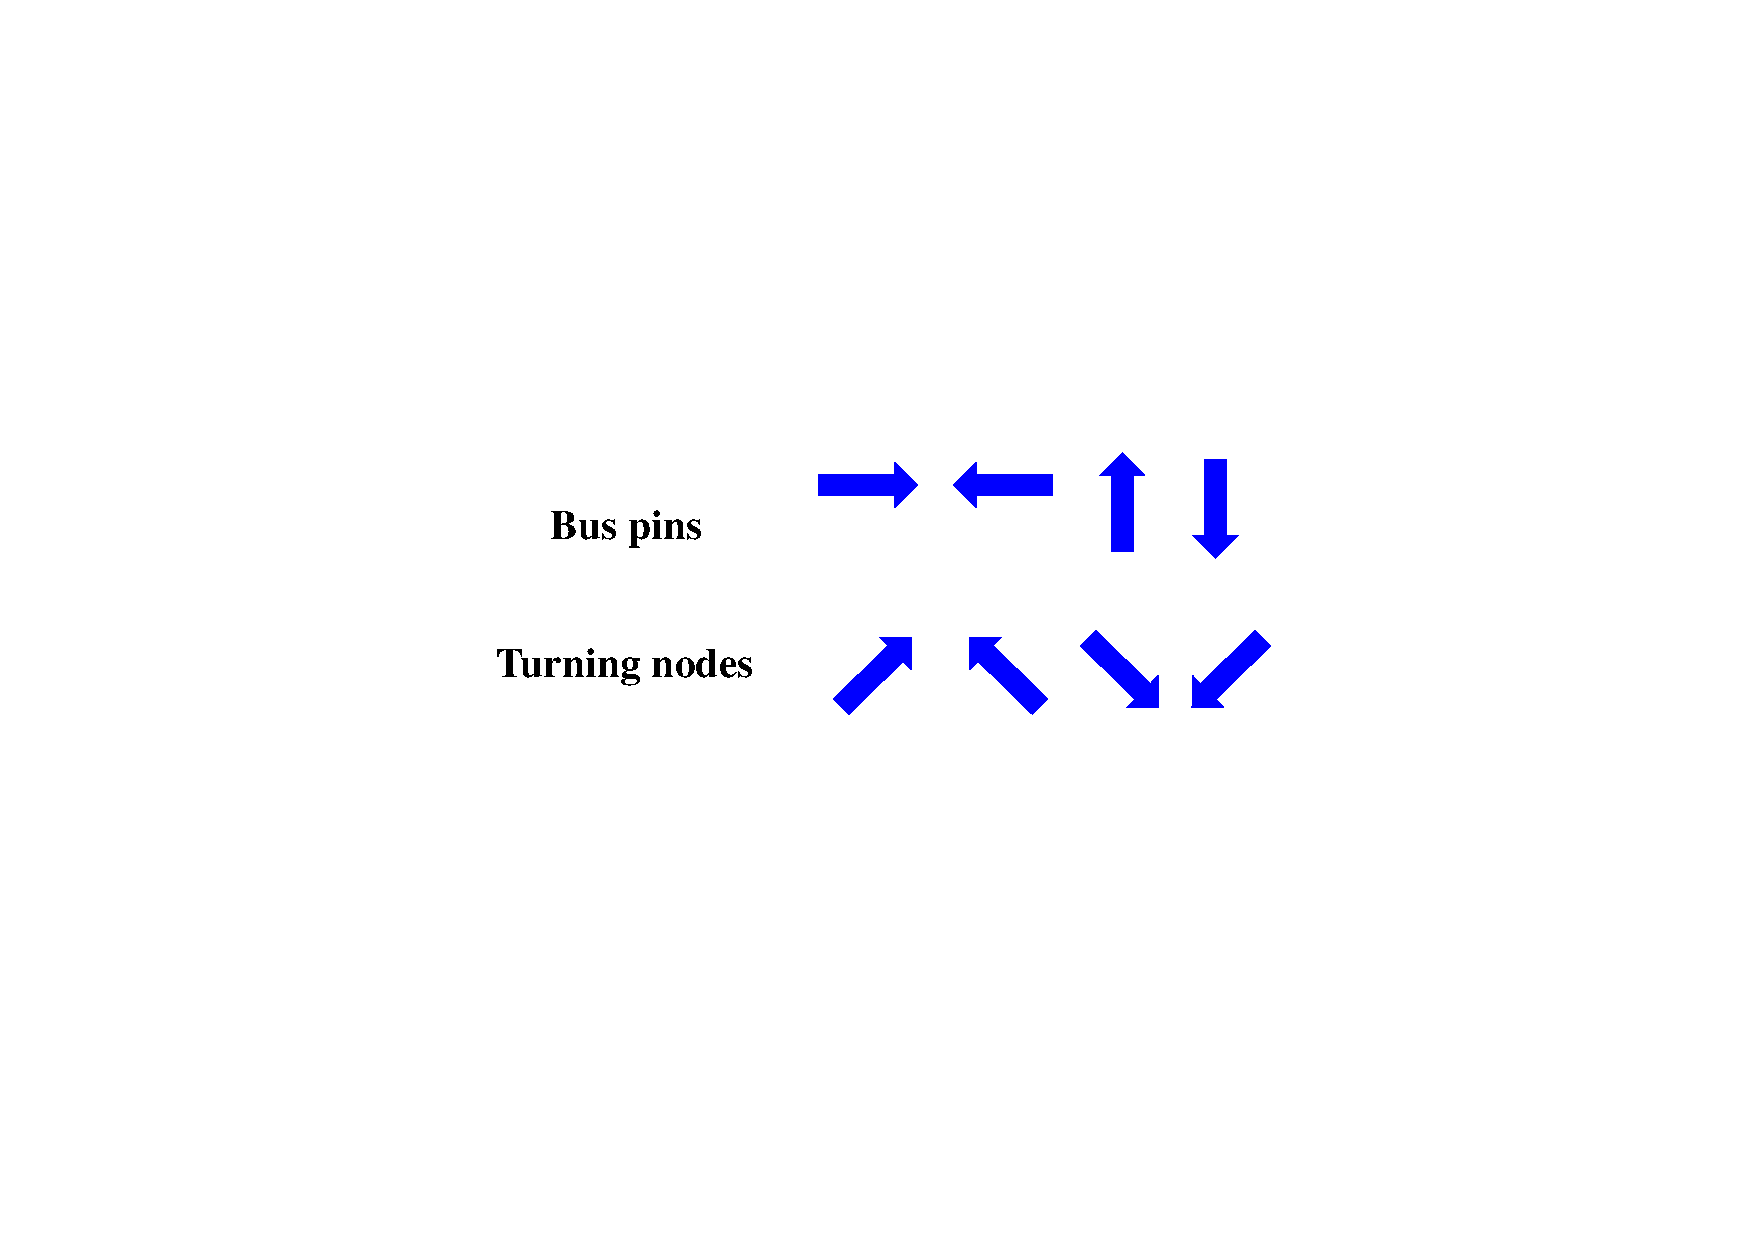
\includegraphics[width=7cm]{Fig/orientation_direction.pdf}
    %\centerline{\psfig{figure=Fig/orientation_direction.eps, width=7cm}}
     \caption{
      The possible orientation directions.
   }
  \label{fig::orientation_direction}
\end{figure}

{\bf Definition 5}: \textbf{\textit{Bus pin flipping}} is used to
change the orientation of the bus pins. In
Figure~\ref{fig::bus_pin_flipping} (a), the orientation of the bus pin
$BP_3$ is from north to south and the orientation of the bus pin
$BP_4$ is from south to north. Since their orientation is opposite and
they are connected with one horizontal bus, the bus twisting makes the signal
wires cross at a point. Furthermore, the bus pin $BP_5$ and $BP_6$ are
connected with a diagonal bus, the orientation of the bus pin $BP_5$ is from
north to south and the orientation of the bus pin $BP_6$ is from west
to east, two extra vias is required at the turning nodes as shown in Figure~\ref{fig::bus_pin_flipping} (a).
All the above problems can be solved
by simply applying bus pin flipping on the bus pins $BP_4$ and $BP_6$.
The result after bus flipping is shown in Figure~\ref{fig::bus_pin_flipping} (b).

{\bf Definition 6}: Wirelength $``$\textbf{\textit{deviation}}$"$
represents the driver-load wirelength difference among all bus bits.
Different choices of the orientations at the bus pins and
turning nodes may cause different driver-load wirelength among all
bits. In this paper, we only need to minimize the wirelength
difference between MSB and LSB of the bus because the wirelength
of all other bits can be linearly interpolated by it. The MSB-LSB
wirelength deviation could be expressed by

\begin{eqnarray}
dev_{len} = | len(MSB) - len(LSB)|
\end{eqnarray}

A turning node can contribute $-$D, 0 or $+$D to the MSB-LSB
wirelength difference, where D = 2$\times$$BW$ and $BW$ is the bus width.
Accumulating the turning node contributions along the path from
the driver to the load of the bus provides $dev_{len}$ at the
load. Figure~\ref{fig::bus_pin_flipping} illustrates the different
deviation results from the different choices at the turning nodes.
In Figure~\ref{fig::bus_pin_flipping} (b), the deviation from the
bus pin $BP_5$ to the bus pin $BP_6$ is $-$D, while in
Figure~\ref{fig::bus_pin_flipping} (a) is 0, but it needs two
extra vias at the turning nodes. Therefore, it is hard to
optimize the total deviation with no extra vias are used at the
turning nodes.

%%%%%%%%%%%%%%%%%%%%%%%%%%
\chapter{Algorithm}
\label{chap::ALGORITHM}
%%%%%%%%%%%%%%%%%%%%%%%%%%

\baselineskip=26pt

\begin{figure}[htb]
  \centering
   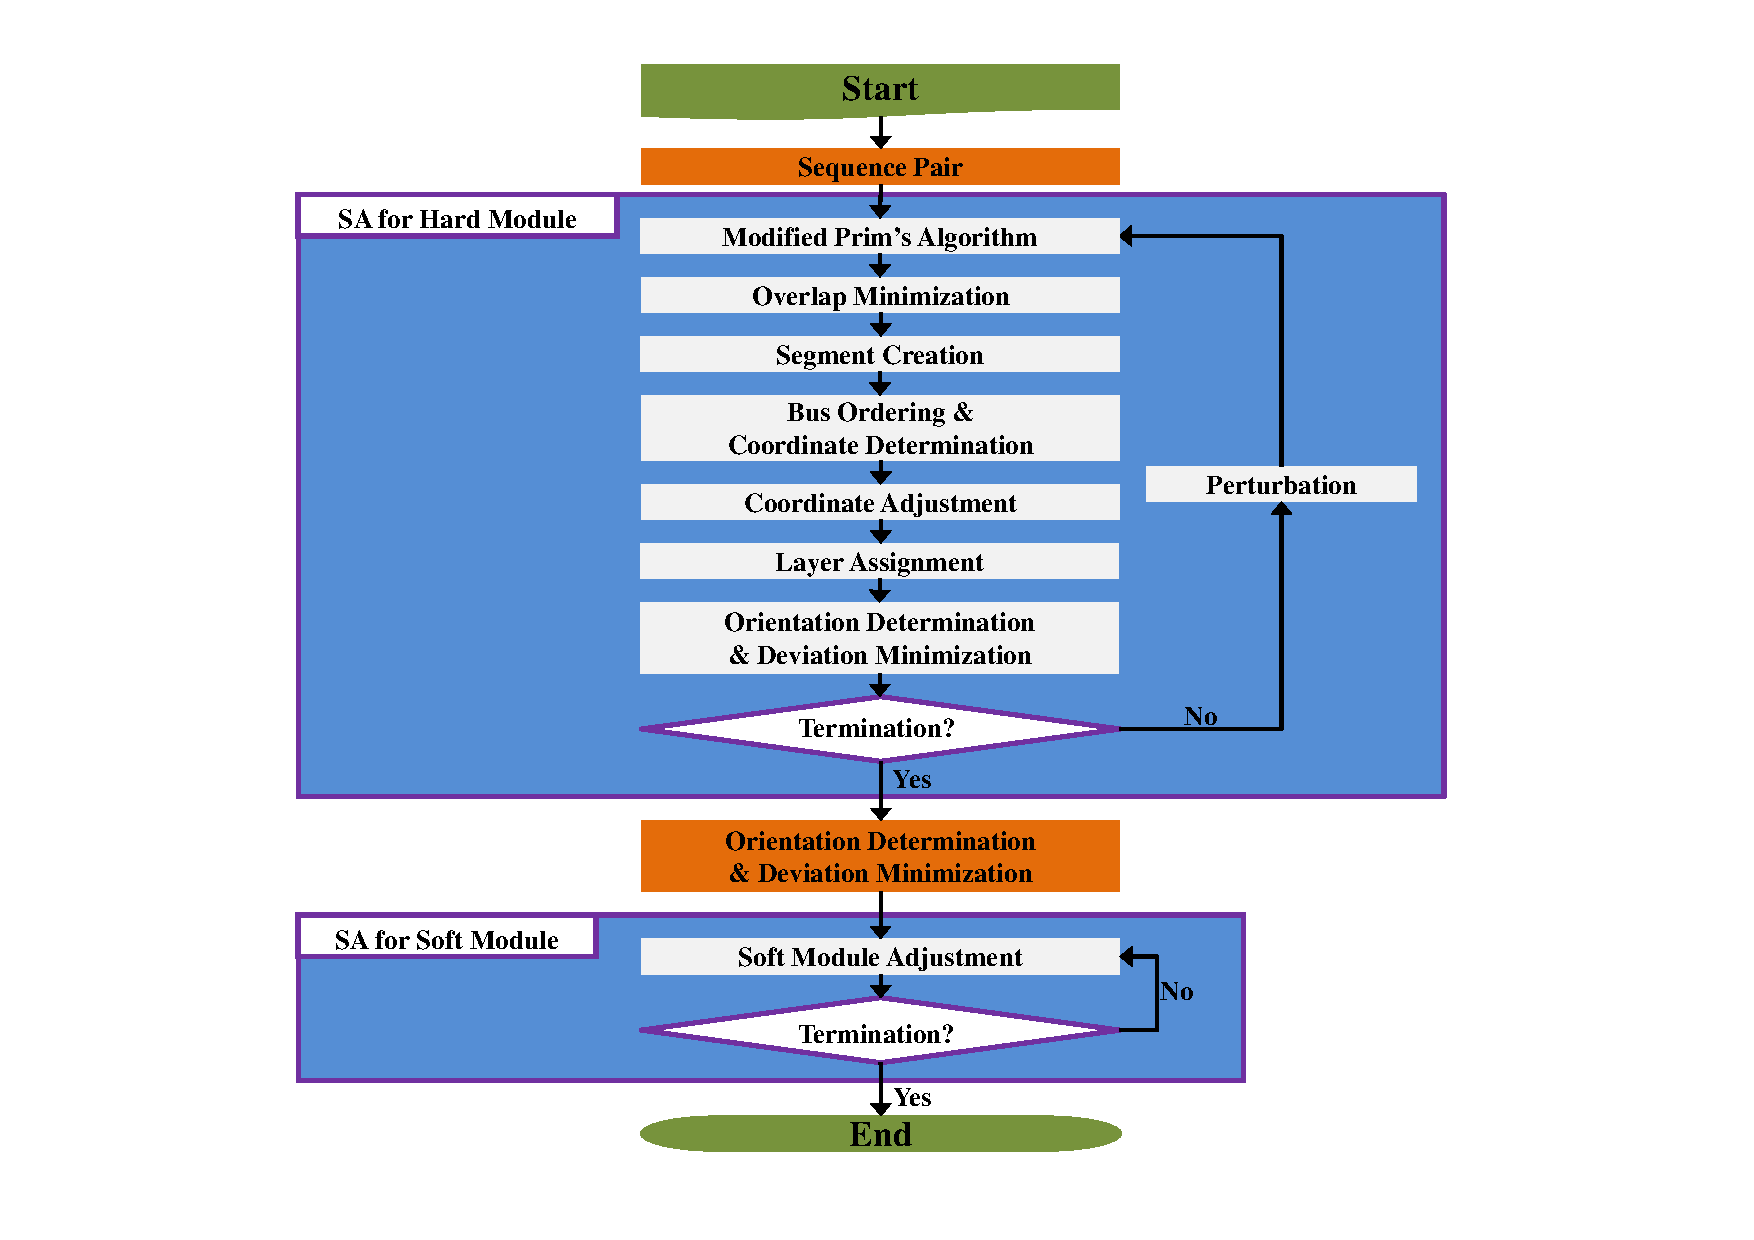
\includegraphics[width=13cm]{Fig/flowchart.pdf}
   %\centerline{\psfig{figure=Fig/flowchart.eps, width=13cm}}
     \caption{
      Algorithm overview.
   }
  \label{fig::flowchart}
\end{figure}

The flowchart of our bus-pin-aware bus-driven floorplanning
algorithm is shown in Figure~\ref{fig::flowchart}.
In the beginning of our algorithm, it derives a floorplan by using
the sequence pair representation \cite{Murata95}, then it computes
the coordinate of each module on the floorplan to obtain the geometric
relations between modules.
Next, the modified Prim's algorithm is used to obtain bus routing topologies,
and it applies the overlap minimization algorithm to minimize the overlap between
different bus components in the MST.
Since some bus pins may not be passed by the buses, it needs to add some buses
for connecting the bus pins to the MST.
After the above steps, several horizontal and vertical buses are obtained,
and their coordinate could be determined. Then, it performs coordinate adjustment algorithm
to further optimize the wirelength by adjusting the coordinate of each bus.
Since extra vias are \textbf{\textit{forbidden}}
at the bend of the diagonal buses, the modified graph coloring algorithm
is used to assign each bus to different layers.
Then the algorithm discussed in the Section~\ref{sec::Fast Deviation Update Based on Topology Comparison}
is used to determine the position and orientation of each bus pin for the current solution, meanwhile, it
minimizes the deviation at each load.

During perturbation, it has three operations to
perturb the current floorplan: (1) Rotate. (2) Reverse. (3) Swap.
The cost function used in this paper is defined as follows:
\begin{eqnarray}
Cost = \alpha \cdot \textbf{\textit{A}} + \beta \cdot
\textbf{\textit{B}} + \gamma \cdot \textbf{\textit{I}}
\end{eqnarray}

where \textbf{\textit{A}} is the chip area, \textbf{\textit{B}} is
the bus area, \textbf{\textit{I}} is the number of invalid bus nets,
$\alpha$, $\beta$, and $\gamma$ are parameters defined by the users.
For saving runtime, it only performs the bus routing algorithm when
the current chip area is smaller than the chip area of the best solution.
Each time a better solution is found, it will check the deviation of
the best solution and the current solution, the solution
with best deviation will be stored.

After the simulated annealing stage, the algorithm discussed in
the Section~\ref{sec::Fast Deviation Update Based on Topology Comparison} is performed to
determine the position and orientation of each bus pin for the best solution. Finally, it changes either the
width or height of the modules lying on the critical path to obtain
a better chip area.

\section{Modified Prim's Algorithm} \label{sec::Modified Prims Algorithm}
To derive the bus topologies, it first constructs the MST for connecting the
bus modules. Since the deviation is calculated from the driver to each load,
to take the impact of the deviation into consideration,
we adopt the Prim's algorithm to construct the MST from
the driver. During constructing the MST, it checks the capacity
of each module to avoid violating capacity constraint. If the selected
edges violate the constraint, then other edges will be chosen to
connect the MST. The bus is regarded as infeasible if no MST is finally
constructed.

\begin{figure}[htb]
  \centering
    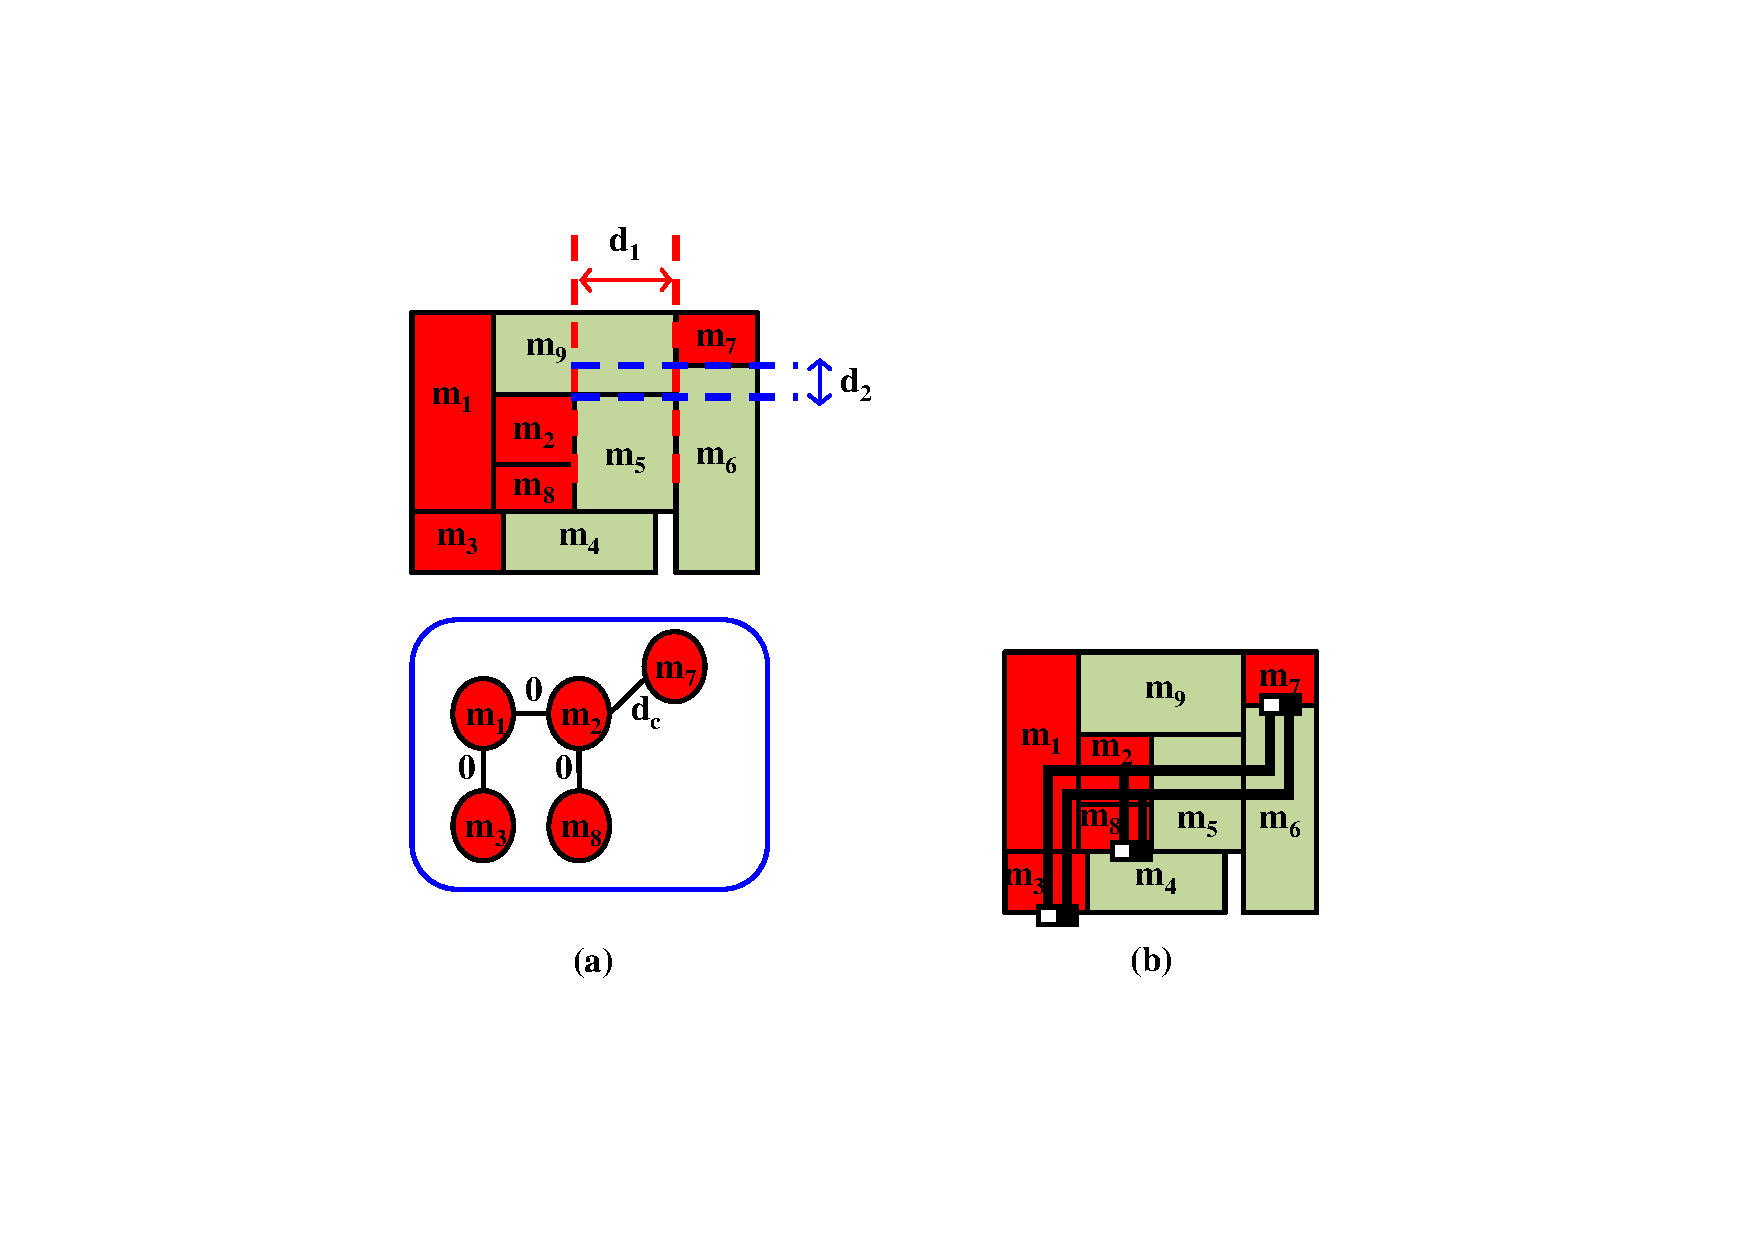
\includegraphics[width=8.8cm]{Fig/MST.pdf}
    %\centerline{\psfig{figure=Fig/MST.eps, width=8.8cm}}
     \caption{
       (a) Minimum spanning tree. (b) The resulting routing tree.
   }
  \label{fig::minimum_spanning_tree}
\end{figure}

Figure~\ref{fig::minimum_spanning_tree} (a) is an example of the
MST. The MST connects the modules $m_1$, $m_2$, $m_3$, $m_7$, and
$m_8$, the weight of each edge is derived from the distance
between different modules. For instance, the weight $d_c$ of the diagonal
bus connecting $m_2$ and $m_7$ is $d_1$ + $d_2$. When determining the
coordinate of each bus, it only handles the horizontal and vertical
buses, thus, each diagonal bus in the MST will be split into one
horizontal and one vertical buses.
Figure~\ref{fig::minimum_spanning_tree} (b) shows the routing
result of Figure~\ref{fig::minimum_spanning_tree} (a).

During constructing the MST, it considers the diagonal connection
between different modules, checks the capacity constraint, and
minimizes the bus wirelength. Therefore, we modify the Prim's algorithm to
meet the above requirements.

\section{Segment Creation}
\label{sec::Segment Creation}

\begin{figure}[htb]
  \centering
    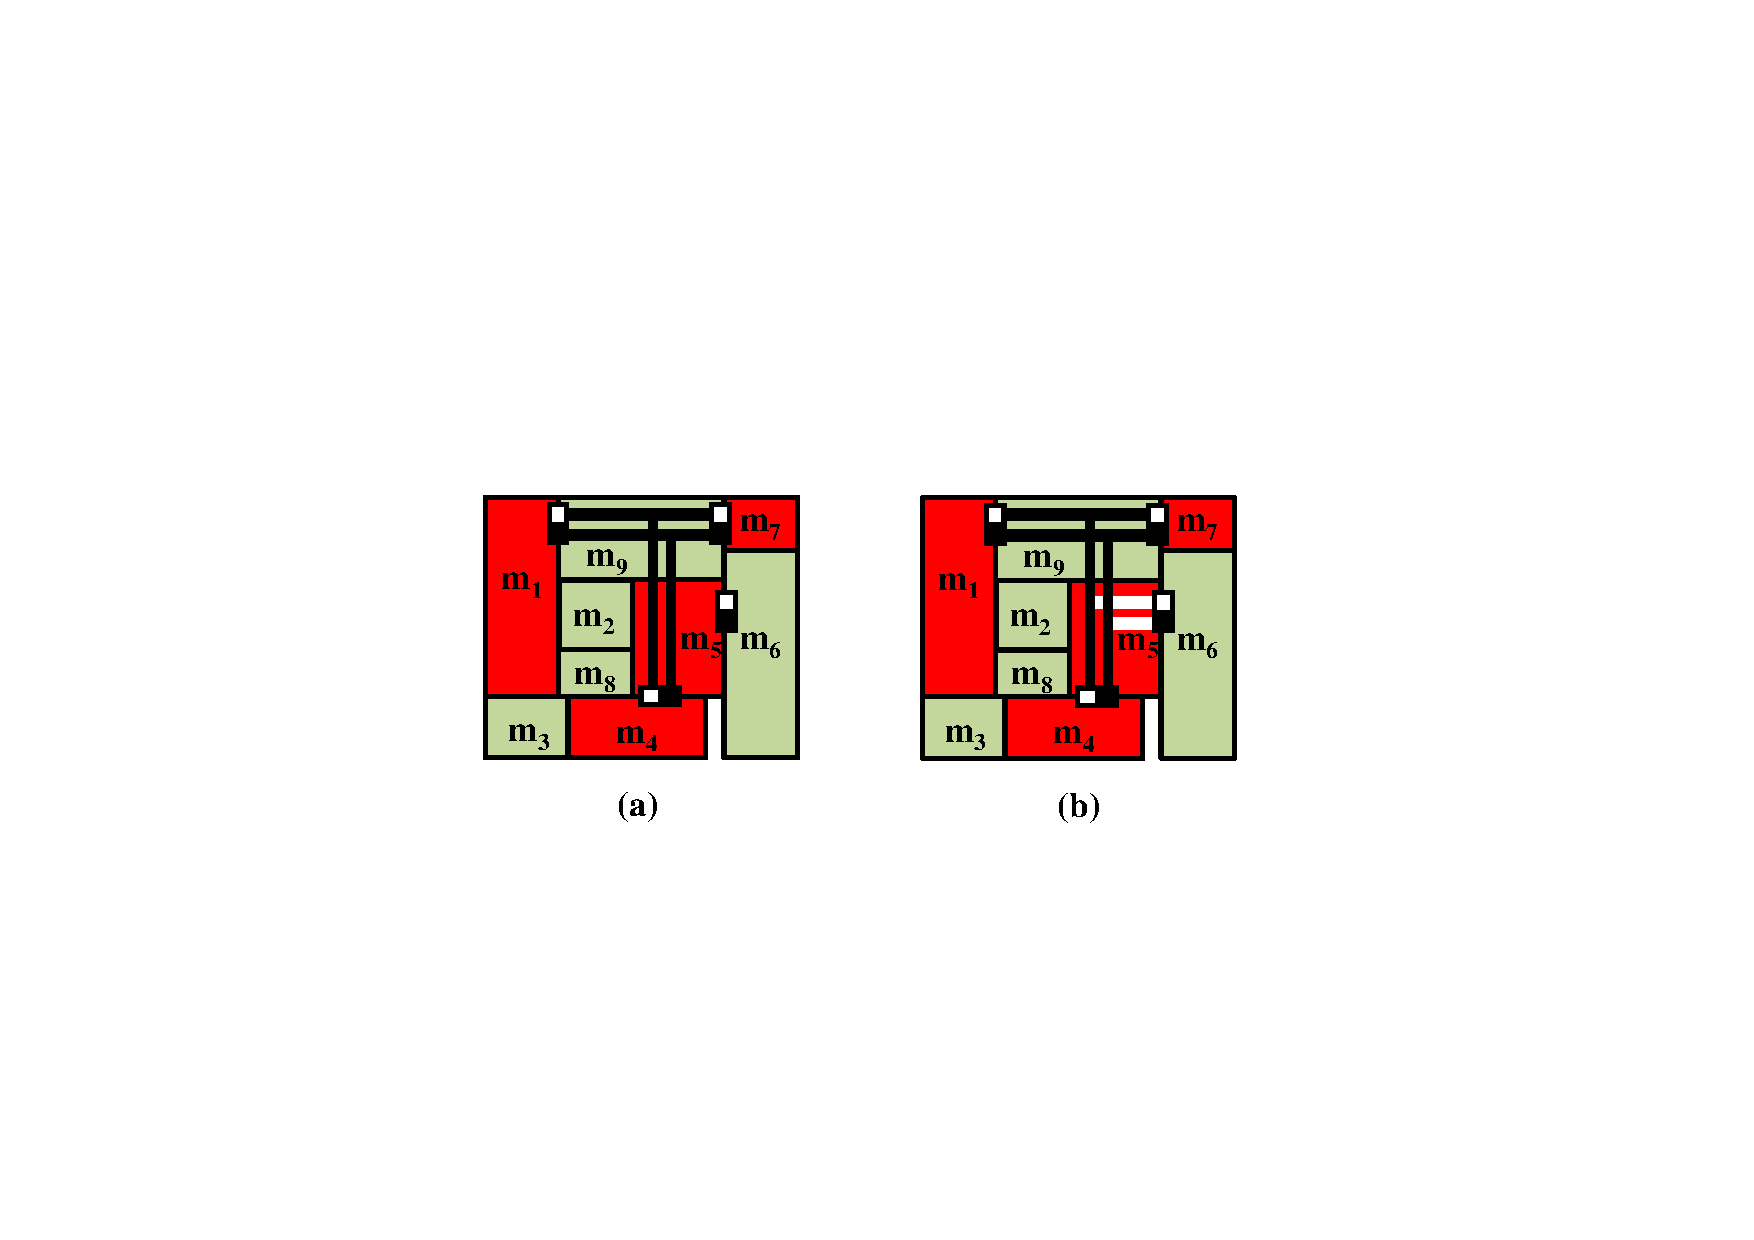
\includegraphics[width=8.8cm]{Fig/segment_creation.pdf}
    %\centerline{\psfig{figure=Fig/segment_creation.eps, width=8.8cm}}
     \caption{
      \small
       (a) Before adding segment. (b) After adding segment.
   }
  \label{fig::segment_creation}
\end{figure}

During constructing the MST, the position of the bus pins is ignored,
as a result, the bus pin of some modules may not be passed by the MST.
To connect the bus pin to the MST, some segments must be added to meet the
requirement. Figure~\ref{fig::segment_creation} (a) is an example, the bus connects four modules $m_1$,
$m_4$, $m_5$, and $m_7$, and the bus pin on module $m_5$ is not passed by the MST.
To solve this problem, one horizontal segment is added for connecting the bus pin on the module $m_5$ to the MST.
The result of segment addition is shown in Figure~\ref{fig::segment_creation} (b).

\section{Bus Ordering and Coordinate Determination}
\label{sec::Bus Ordering and Coordinate Determination}
\subsection{Bus Ordering} \label{sec::Bus Ordering}
Since the coordinate of each bus is determined in non-decreasing
order, it finds the bus ordering of all horizontal (vertical)
buses and determines the coordinate of each bus according to the
bus ordering \cite{Xiang03}. Given a sequence pair, it can obtain the relative
position of any two modules, and the ordering of any two buses is
derived from the relative position of those modules passed by the
buses.

\begin{figure}[htb]
  \centering
    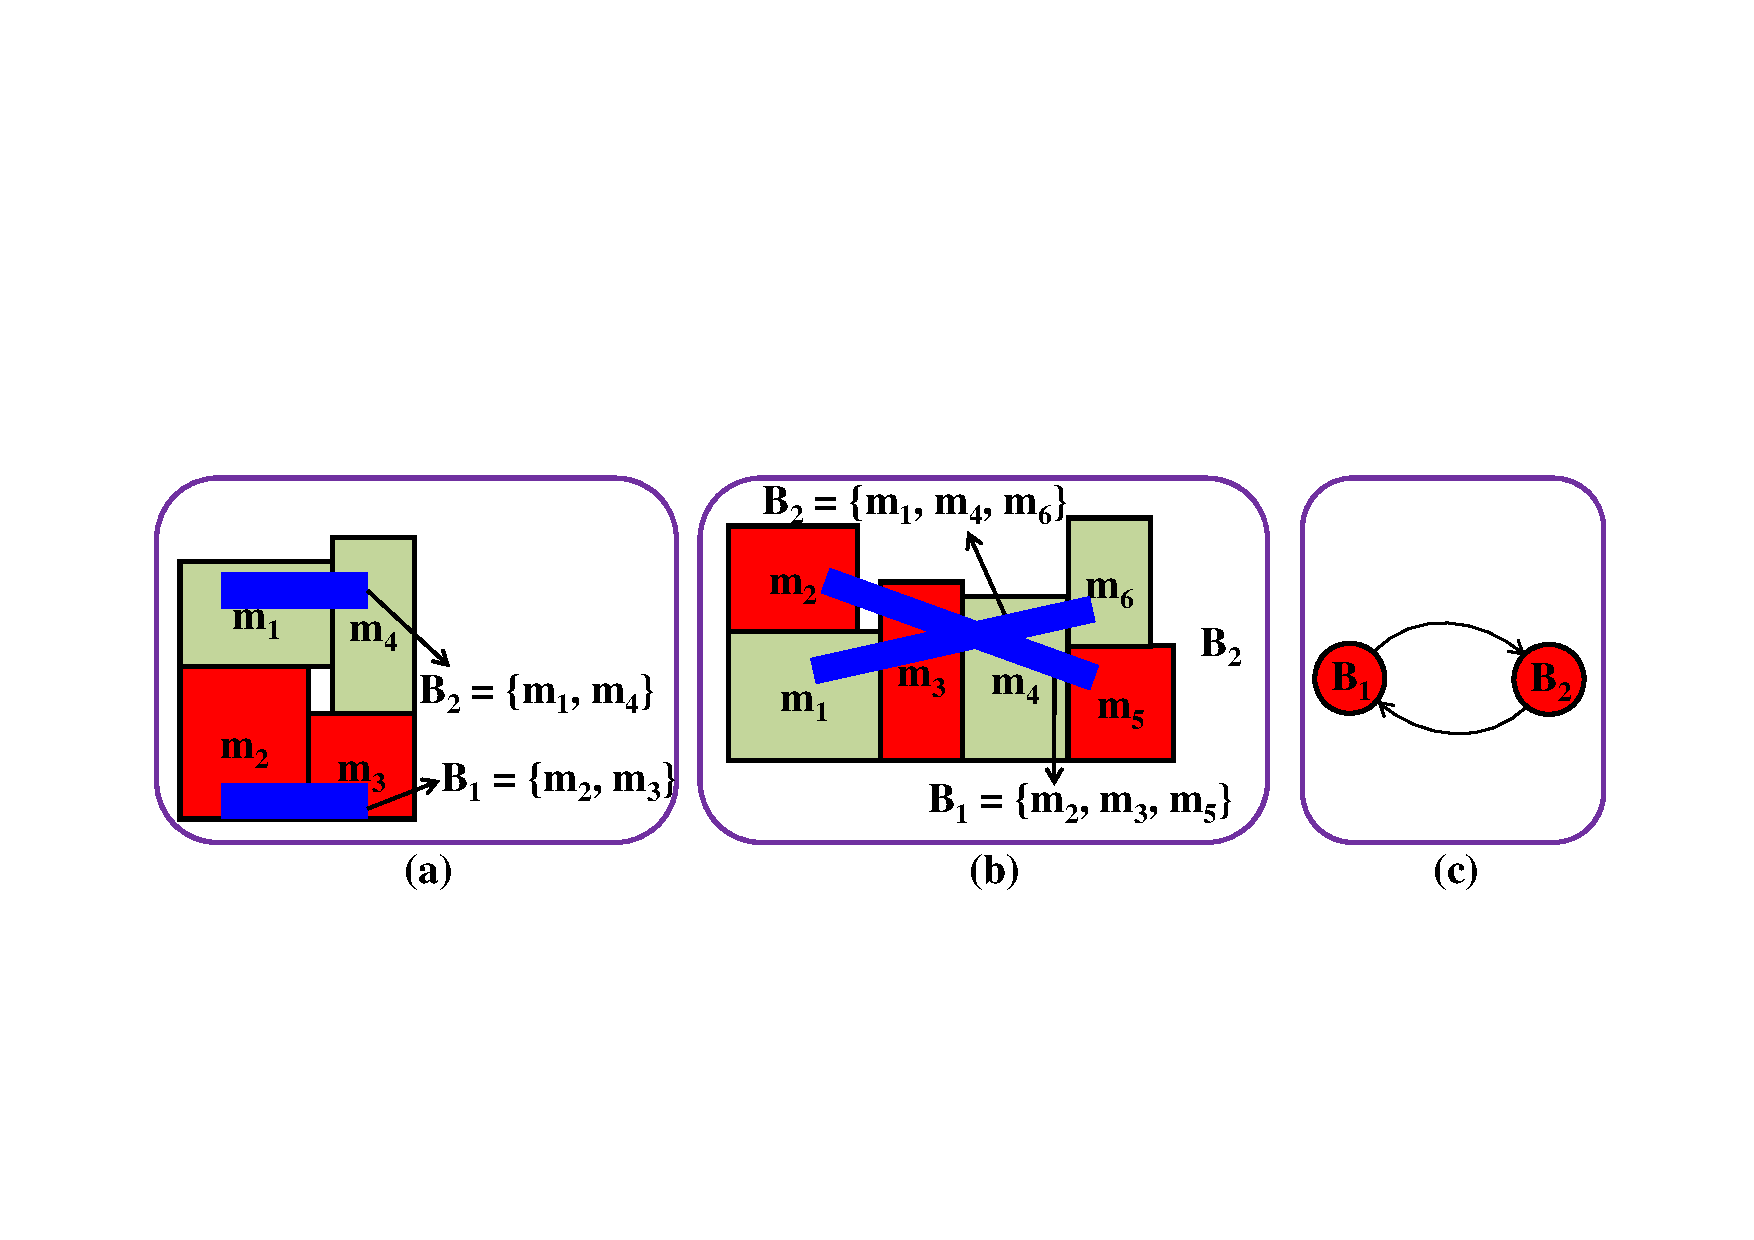
\includegraphics[width=12cm]{Fig/bus_ordering.pdf}
    %\centerline{\psfig{figure=Fig/bus_ordering.eps, width=12cm}}
     \caption{
       (a) Bus ordering. (b) Bus crossing. (c) Ordering constraint graph.
   }
  \label{fig::bus_ordering}
\end{figure}

Figure~\ref{fig::bus_ordering} (a) gives an example. The sequence
pair of the floorplan is (1243, 2314), two buses $B_1$ = \{$m_2$,
$m_3$\} and $B_2$ = \{$m_1$, $m_4$\} are placed on the floorplan.
The module $m_1$ is placed above the module $m_2$ according to the
sequence pair, thus, the bus $B_2$ passing through the module
$m_1$ has to be placed above the bus $B_1$ passing through the
module $m_2$. This condition is called $bus\ ordering$.
In order to obtain the bus ordering between any two buses, it
constructs the ordering constraint graph (OCG) by performing the
above steps on any two horizontal (vertical) buses. The buses are
represented as the nodes in the OCG, and the edges represent the
ordering between any two buses.

During determining the bus ordering, different buses may conflict
with each other. In Figure~\ref{fig::bus_ordering} (b), two buses
$B_1$ = \{$m_2$, $m_3$, $m_5$\} and $B_2$ = \{$m_1$, $m_4$,
$m_6$\} are placed on the floorplan. Based on the sequence
pair, the module $m_2$ is placed above the module $m_1$, and the
module $m_6$ is placed above the module $m_5$. Since the modules
$m_1$ and $m_2$ are passed by the buses $B_2$ and $B_1$,
respectively, an edge from the node $B_1$ to the node $B_2$ is
inserted into the OCG. Besides, the modules $m_5$ and $m_6$
are passed by the buses $B_1$ and $B_2$, respectively, an edge
from node $B_2$ to node $B_1$ is inserted into the OCG. Thus, the OCG
contains a cycle as shown in Figure~\ref{fig::bus_ordering} (c).
It means that two buses conflict with each other, and one of the
two buses is regarded as infeasible. This situation is called
$bus\ crossing$.

To determine the bus ordering of all horizontal (vertical) buses
from the OCG, we first set the nodes with zero out-degree in the
OCG the highest priority comparing with remaining horizontal
(vertical) buses. By this property, it determines the bus ordering
by deleting the nodes and edges from the OCG iteratively. In each
iteration, it removes the node with zero out-degree and deletes
the edges connecting to it from the OCG. If no such node in the
OCG, it means that the cycle is contained in the OCG and one of the
minimum out-degree nodes is regarded as infeasible. Then the
invalid node and the edges connecting to it will be deleted from
the OCG. The above steps are repeated until all nodes are removed
from the OCG. Finally, the bus ordering of all feasible horizontal
(vertical) buses can be obtained.
\subsection{Coordinate Determination}
\label{sec::Coordinate Determination} After determining the bus ordering, it
starts to determine the coordinate of all horizontal (vertical)
buses \cite{Xiang03}. Without loss of generality, we take the horizontal buses
for example. The coordinate of each horizontal bus $B_i$ is
$y_{max}$ = max\{$y_i$ $|$ $i$ = 1, 2, ..., k\}, where k is the
number of the modules passed by the bus, and $y_i$ is the y
coordinate of each module. If some modules are not passed by the bus $B_i$.
It adjusts the coordinate of each module slightly
such that all modules can be passed by the bus $B_i$.

 \begin{figure}[htb]
  \centering
    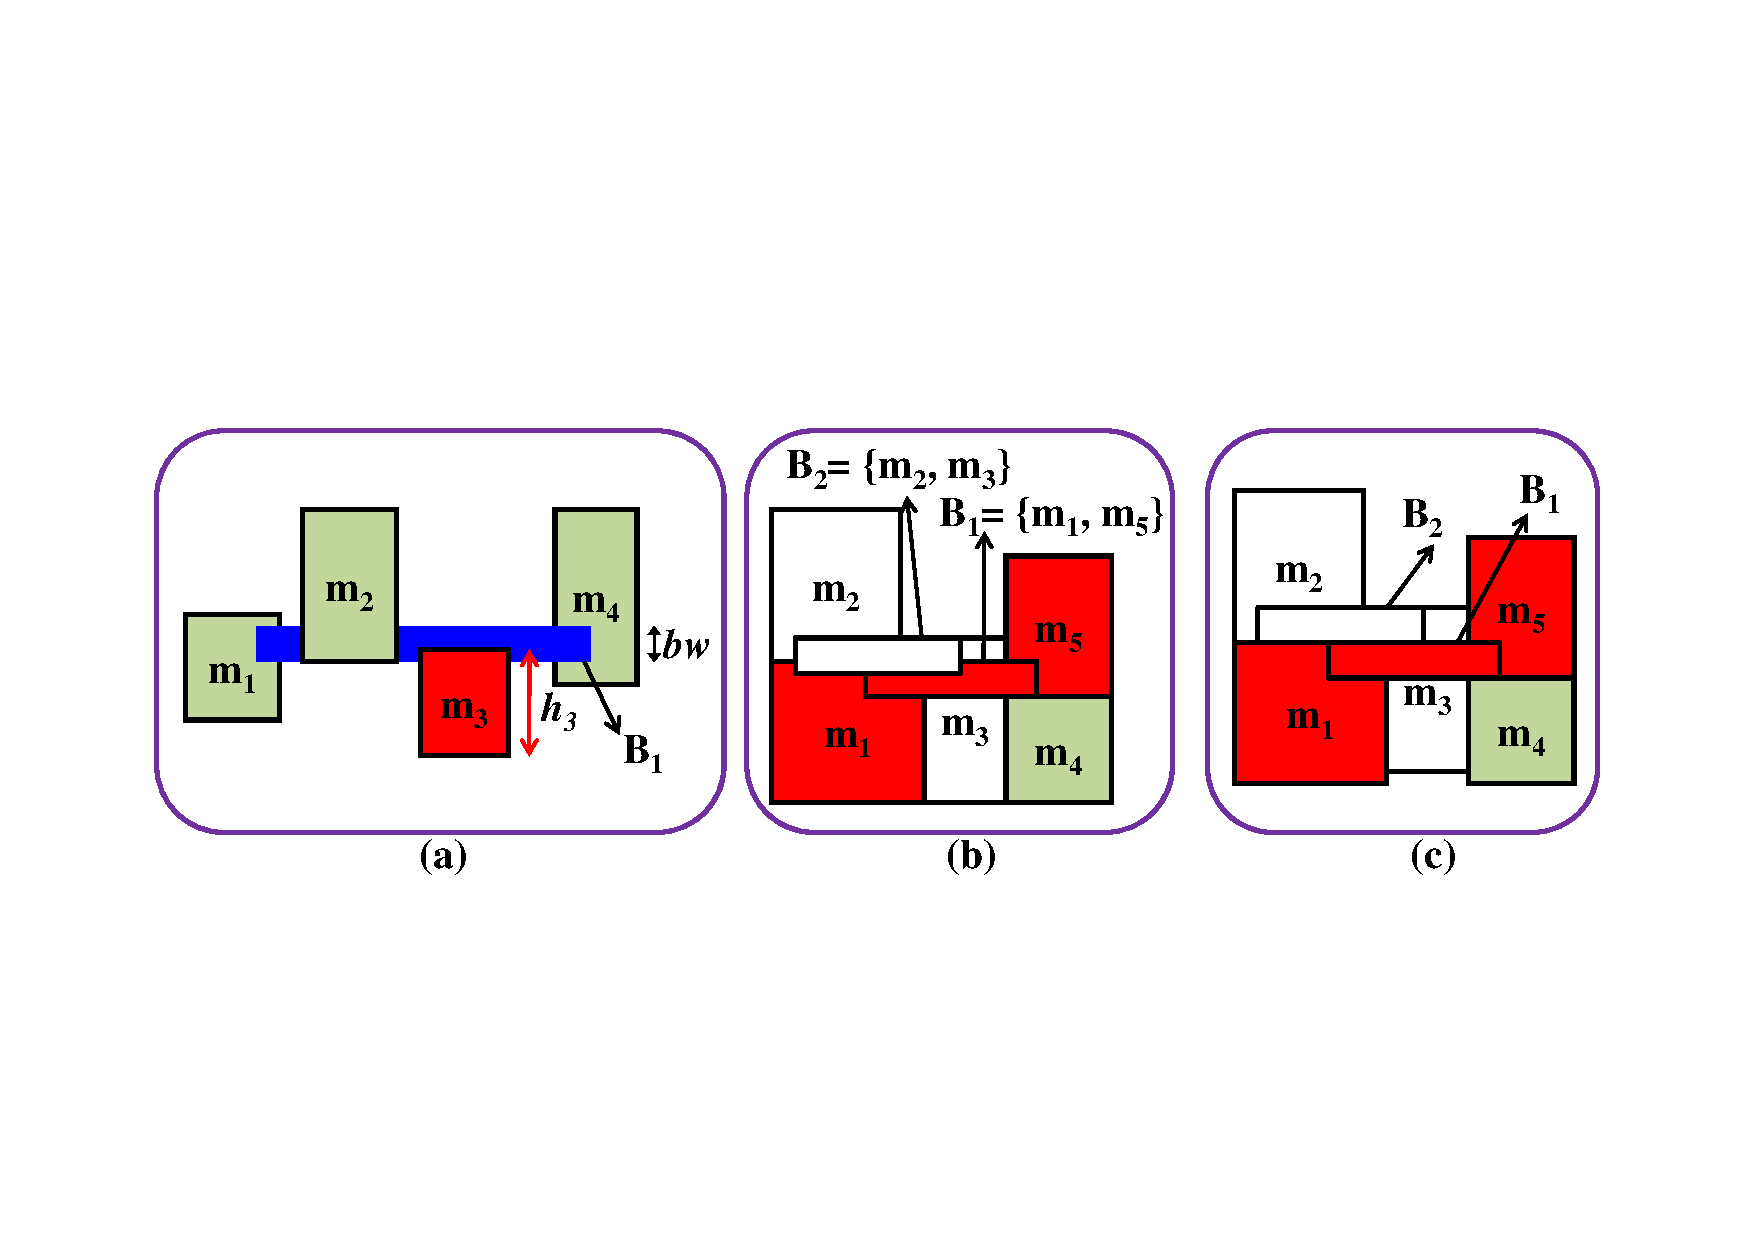
\includegraphics[width=12cm]{Fig/bus_overlapping.pdf}
    %\centerline{\psfig{figure=Fig/bus_overlapping.eps, width=12cm}}
     \caption{
       (a) Module moving. (b) Bus overlapping. (c) No bus overlapping.
   }
  \label{fig::bus_overlapping}
\end{figure}

In Figure~\ref{fig::bus_overlapping} (a), the bus $B_1$ goes
through the modules in \{$m_1$, $m_2$, $m_3$, $m_4$\}, the bus
width of $B_1$ is $bw$, the height of the module $m_i$ is $h_i$.
In this figure, the coordinate of $B_1$ is $y_{max}$ = max\{$y_i$
$|$ $i$ = 1, 2, 3, 4\}. Since the module $m_3$ is not passed by the
bus $B_1$, it changes the coordinate of the module $m_3$
slightly such that it can be passed by $B_1$, the new coordinate
of $m_3$ is $y_{max}$ + $bw$ - $h_3$.

When considering multiple horizontal (vertical) buses, different
horizontal (vertical) buses may overlap with each other. In
Figure~\ref{fig::bus_overlapping} (b), the buses $B_1$ = \{$m_1$,
$m_5$\} and $B_2$ = \{$m_2$, $m_3$\} are placed on the floorplan.
The bus $B_2$ overlaps with the bus $B_1$ on the floorplan, this
situation is called $bus\ overlapping$. Therefore, the bus $B_2$ has
to be moved up until there is no overlap with the buses below. The result is shown in
Figure~\ref{fig::bus_overlapping} (c).

\section{Wirelength Reduction}
\subsection{Overlap Minimization}
\label{sec::Overlap Minimization}
Since the width and height of each module is not considered during constructing the MST,
the bus wirelength may be further optimized. In this paper,
we propose an algorithm to reduce the overlap in MST such that
the better bus wirelength could be obtained.

\begin{figure}[htb]
  \centering
    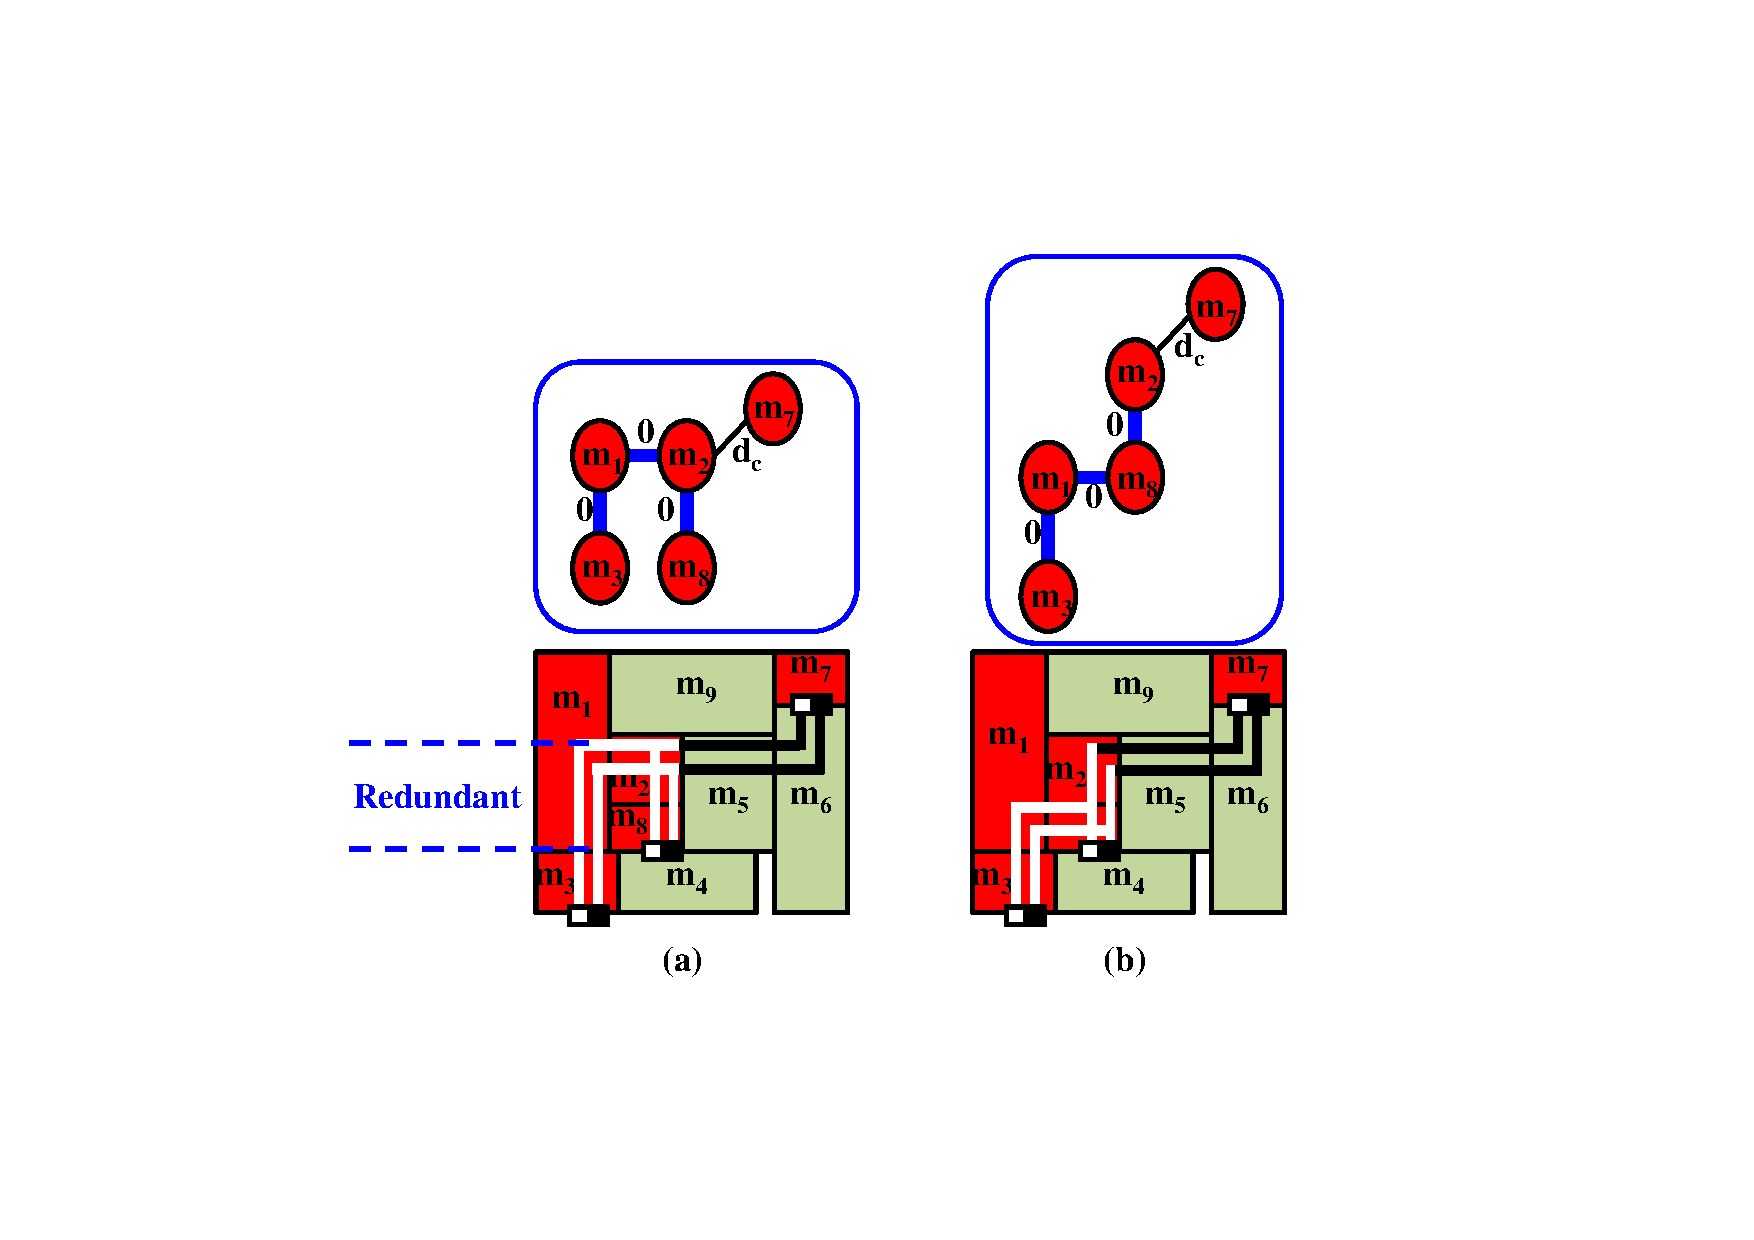
\includegraphics[width=11cm]{Fig/overlap_minimization.pdf}
    %\centerline{\psfig{figure=Fig/overlap_minimization.eps, width=11cm}}
     \caption{
      \small
       (a) Before wirelength reduction. (b) After wirelength reduction.
   }
  \label{fig::overlap_minimization}
\end{figure}

Figure~\ref{fig::overlap_minimization} illustrates how
the algorithm works. The bus connects the five modules $m_1$,
$m_2$, $m_3$, $m_7$, and $m_8$. In Figure~\ref{fig::overlap_minimization} (a),
there are three bus components which form the U-shaped pattern --- one vertical bus component
connects modules $m_1$ and $m_3$, another vertical bus component connects
modules $m_2$ and $m_8$, and the horizontal bus component connects modules
$m_1$ and $m_2$. If the overlap in the U-shaped pattern can be minimized, then
total bus wirelength can be further optimized.
Thus, the horizontal bus component is shifted down to minimize the overlap between the buses.
Figure~\ref{fig::overlap_minimization} (b) demonstrates the
result of wirelength reduction. All the above steps are repeated until all horizontal and vertical
bus components are searched.

\begin{Lemma}
Minimize the overlap in the obtained MST will further decrease the
total bus wirelength of the MST.
\end{Lemma}

\begin{figure}[htb]
  \centering
    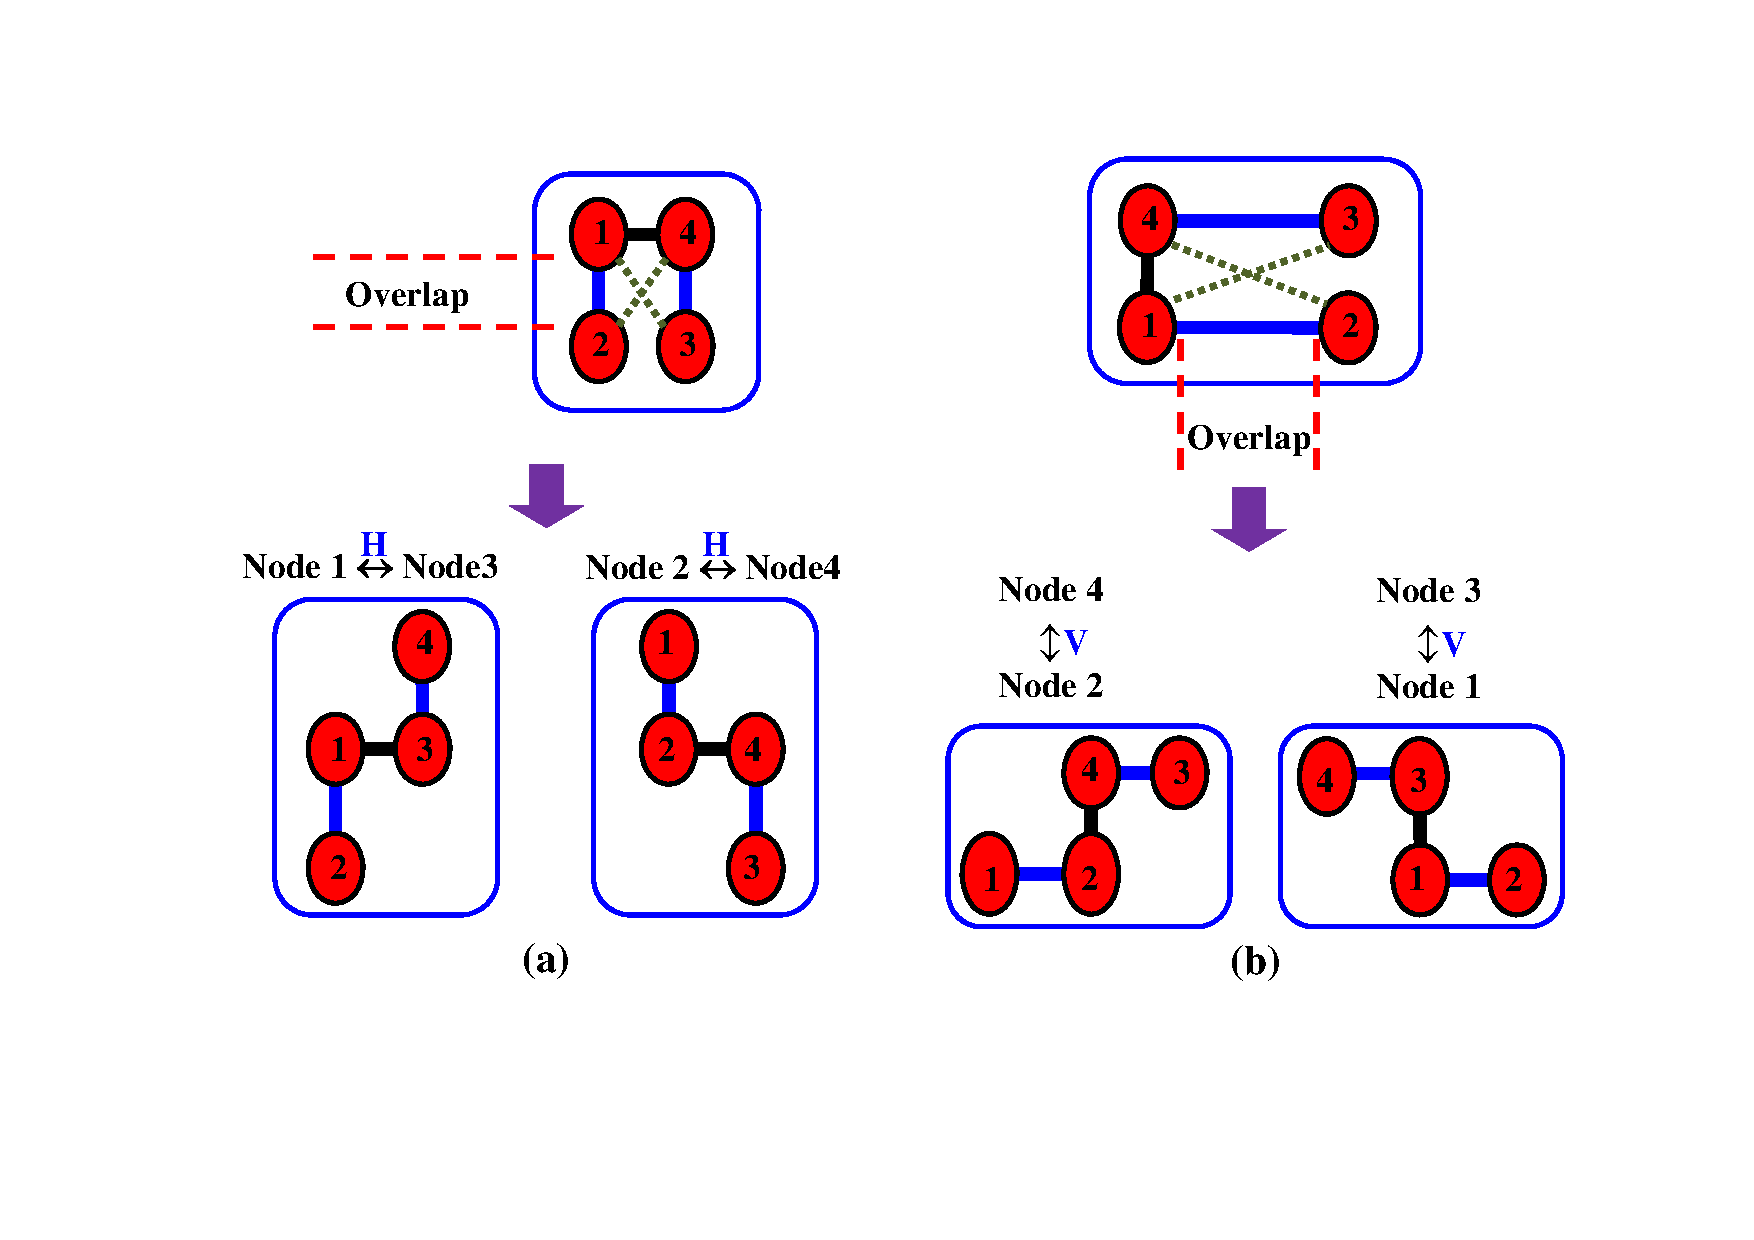
\includegraphics[width=12cm]{Fig/lemma1.pdf}
    %\centerline{\psfig{figure=Fig/lemma1.eps, width=12cm}}
     \caption{
      \small
       (a) Reduction rule for horizontal bus components. (b) Reduction rule for vertical bus components.
   }
  \label{fig::lemma1}
\end{figure}

During constructing the MST for each bus, it ignores the actual information
on the width and height of the module, as a result, the wirelength of the obtained MST may
be further optimized.
For each bus, it will construct a MST.
In each MST, the bus modules are represented as the nodes, and the bus components are represented as the edges.
If one MST contains the U-shaped bus pattern, it means that
there is a overlap in the MST. Therefore, the bus wirelength can be minimized by minimizing the overlap in the MST.

Figure~\ref{fig::lemma1} shows the reduction rule.
In Figure~\ref{fig::lemma1} (a), it shows the reduction rule for the horizontal bus components.
Each time a matched U-shaped patten is found, it will check either
the node 1 is horizontal with the node 3 or the node 2 is horizontal with the node 4.
If the node 1 is horizontal with node 3, then the horizontal bus component connecting
the node 1 and 4 is changed to connect the node 1 and node 3.
If the node 2 is horizontal with node 4, then the horizontal bus component connecting
the node 1 and 4 is changed to connect the node 2 and node 4.
Then, the overlap is minimized to improve the bus wirelength.
Figure~\ref{fig::lemma1} (b) shows the reduction rule for the vertical bus components.
The rule can be derived similarly.

\subsection{Coordinate Adjustment}
\label{sec::Coordinate Adjustment}
When determining the coordinate of each bus, it only focuses on
making each horizontal (vertical) buses feasible but not on
minimizing the bus wirelength. However, different coordinates of
each bus result in different interconnect wirelength
between the horizontal and vertical bus components.
Therefore, the bus wirelength can be further optimized
by properly adjusting the coordinate of each bus component.

\begin{figure}[htb]
  \centering
    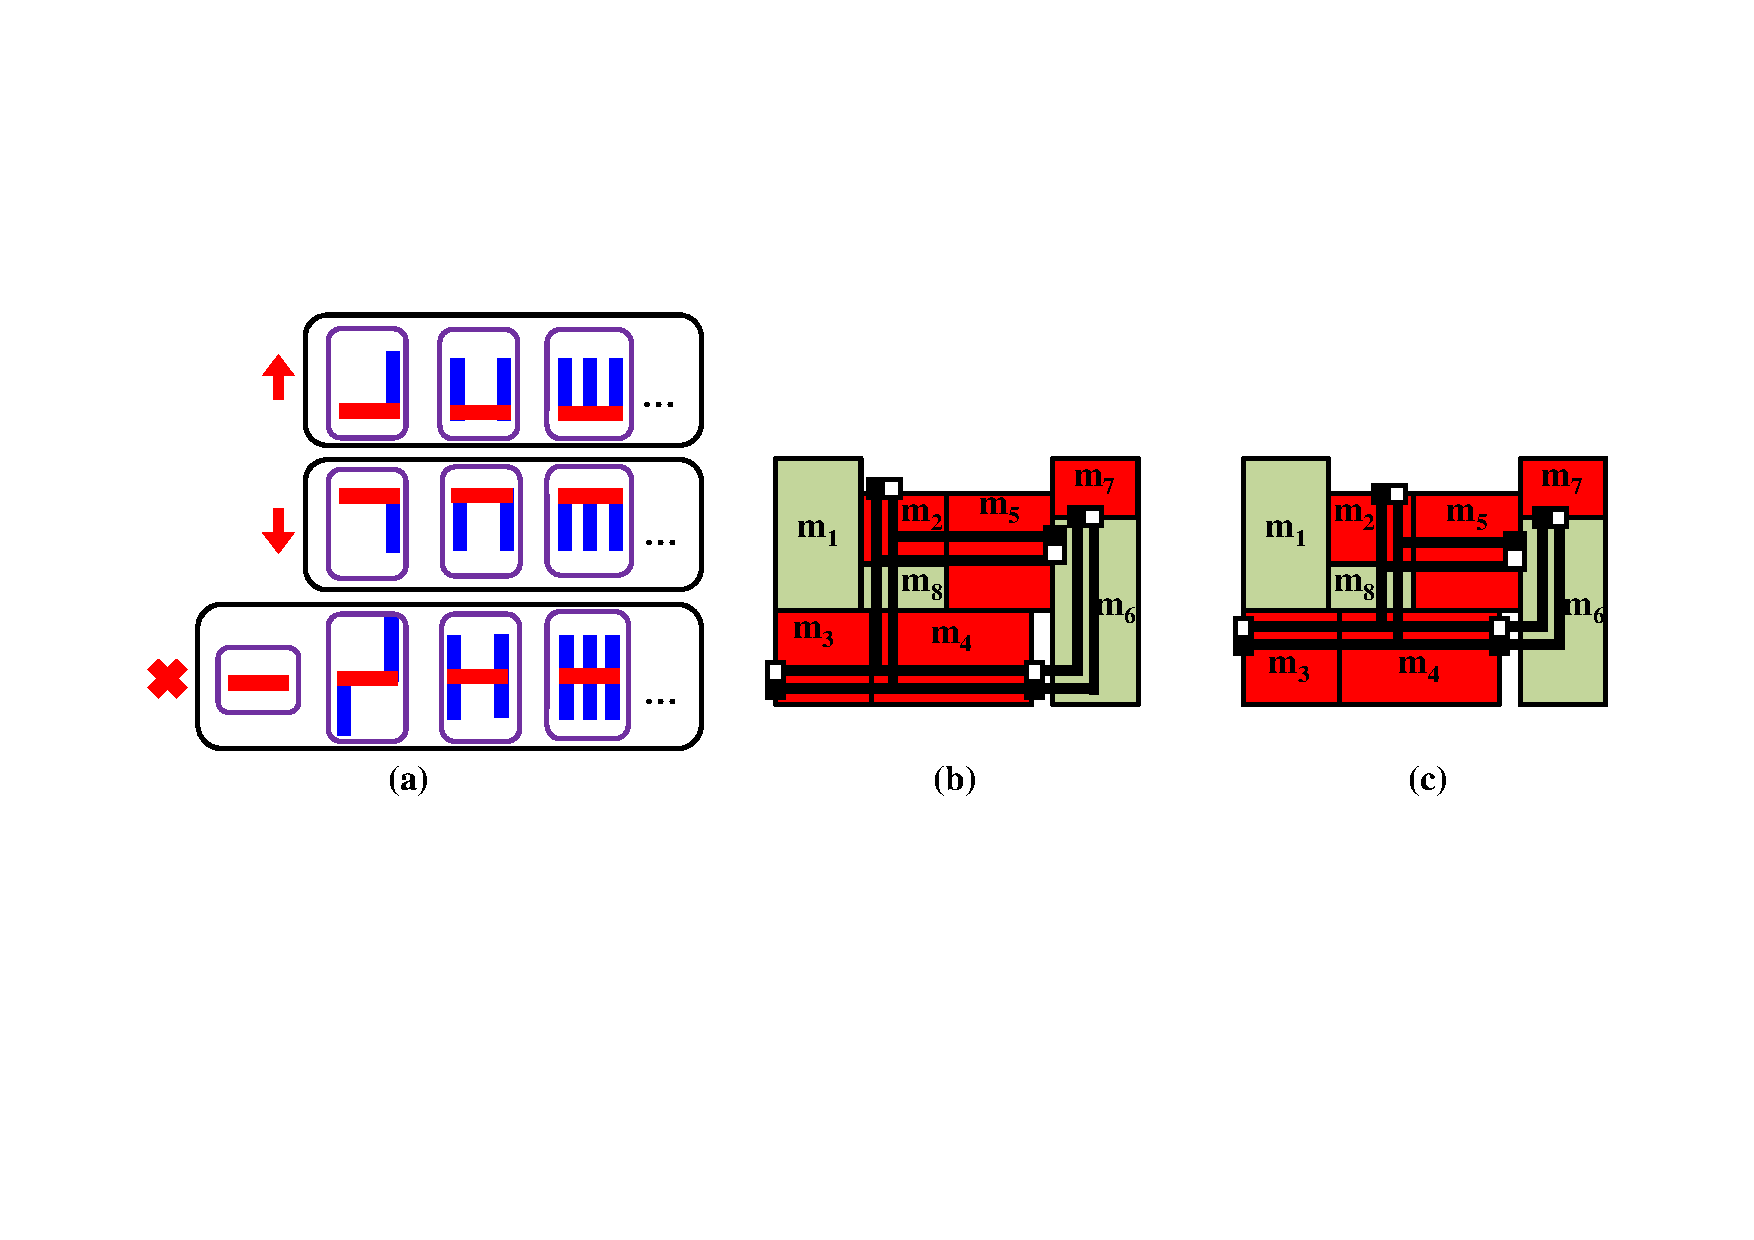
\includegraphics[width=14cm]{Fig/coordinate_adjustment.pdf}
    %\centerline{\psfig{figure=Fig/coordinate_adjustment.eps, width=14cm}}
     \caption{
       (a) Wirelength reduction rule. (b) Before wirelength reduction. (c) After wirelength reduction.
   }
  \label{fig::coordinate_adjustment}
\end{figure}

Figure~\ref{fig::coordinate_adjustment}
(a) illustrates how it works, the horizontal bus component is the target to
be reduced the interconnect wirelength. In the first row, the number of the
vertical bus components intersecting with the horizontal bus component in upper side are
more than in lower side. Thus, it moves the horizontal bus component toward
the upper side to improve its wirelength. In the second row, the
number of the vertical bus components intersecting with the horizontal bus component in
lower side are more than in upper side. Thus, it moves the
horizontal bus component toward the lower side to improve its wirelength. In
the third row, the number of the vertical bus components intersecting with the
horizontal bus component are equal on both side, thus, the coordinate of the horizontal
bus component is not changed.

In Figure~\ref{fig::coordinate_adjustment} (b), the bus = \{$m_2$, $m_3$, $m_4$, $m_5$, $m_7$\}
is placed on the floorplan. Assume we first checks the horizontal bus \{$m_3$, $m_4$\}.
According to the rule as shown in Figure~\ref{fig::coordinate_adjustment} (a), it reduces the wirelength by
moving the bus toward the upper side of the floorplan. The above steps are repeated until all horizontal
and vertical buses are applied, the optimized result is demonstrated in Figure~\ref{fig::coordinate_adjustment} (c).

\begin{Lemma}
Under some specific bus topologies, different positions of each horizontal (vertical) bus
would result in different bus wirelength.
\end{Lemma}

As mentioned earlier, the coordinate of each horizontal bus component is assigned to the highest y-coordinate
of all connected bus modules, and the coordinate of each vertical bus component is assigned to the highest
x-coordinate of all connected bus modules. However, different coordinate of the bus components
result in different interconnect wirelength between the horizontal and vertical bus components.
If the coordinate of each bus component is not carefully assigned,
then the total bus wirelength will be increased dramatically. Nevertheless,
the task is more complicated if it determines the best position of all
horizontal (vertical) bus components simultaneously. Therefore, a better approach is to
decide an initial position for each horizontal (vertical) bus component, then it adjusts
the coordinate of each bus component such that the better bus wirelength can be achieved.

\begin{figure}[htb]
  \centering
    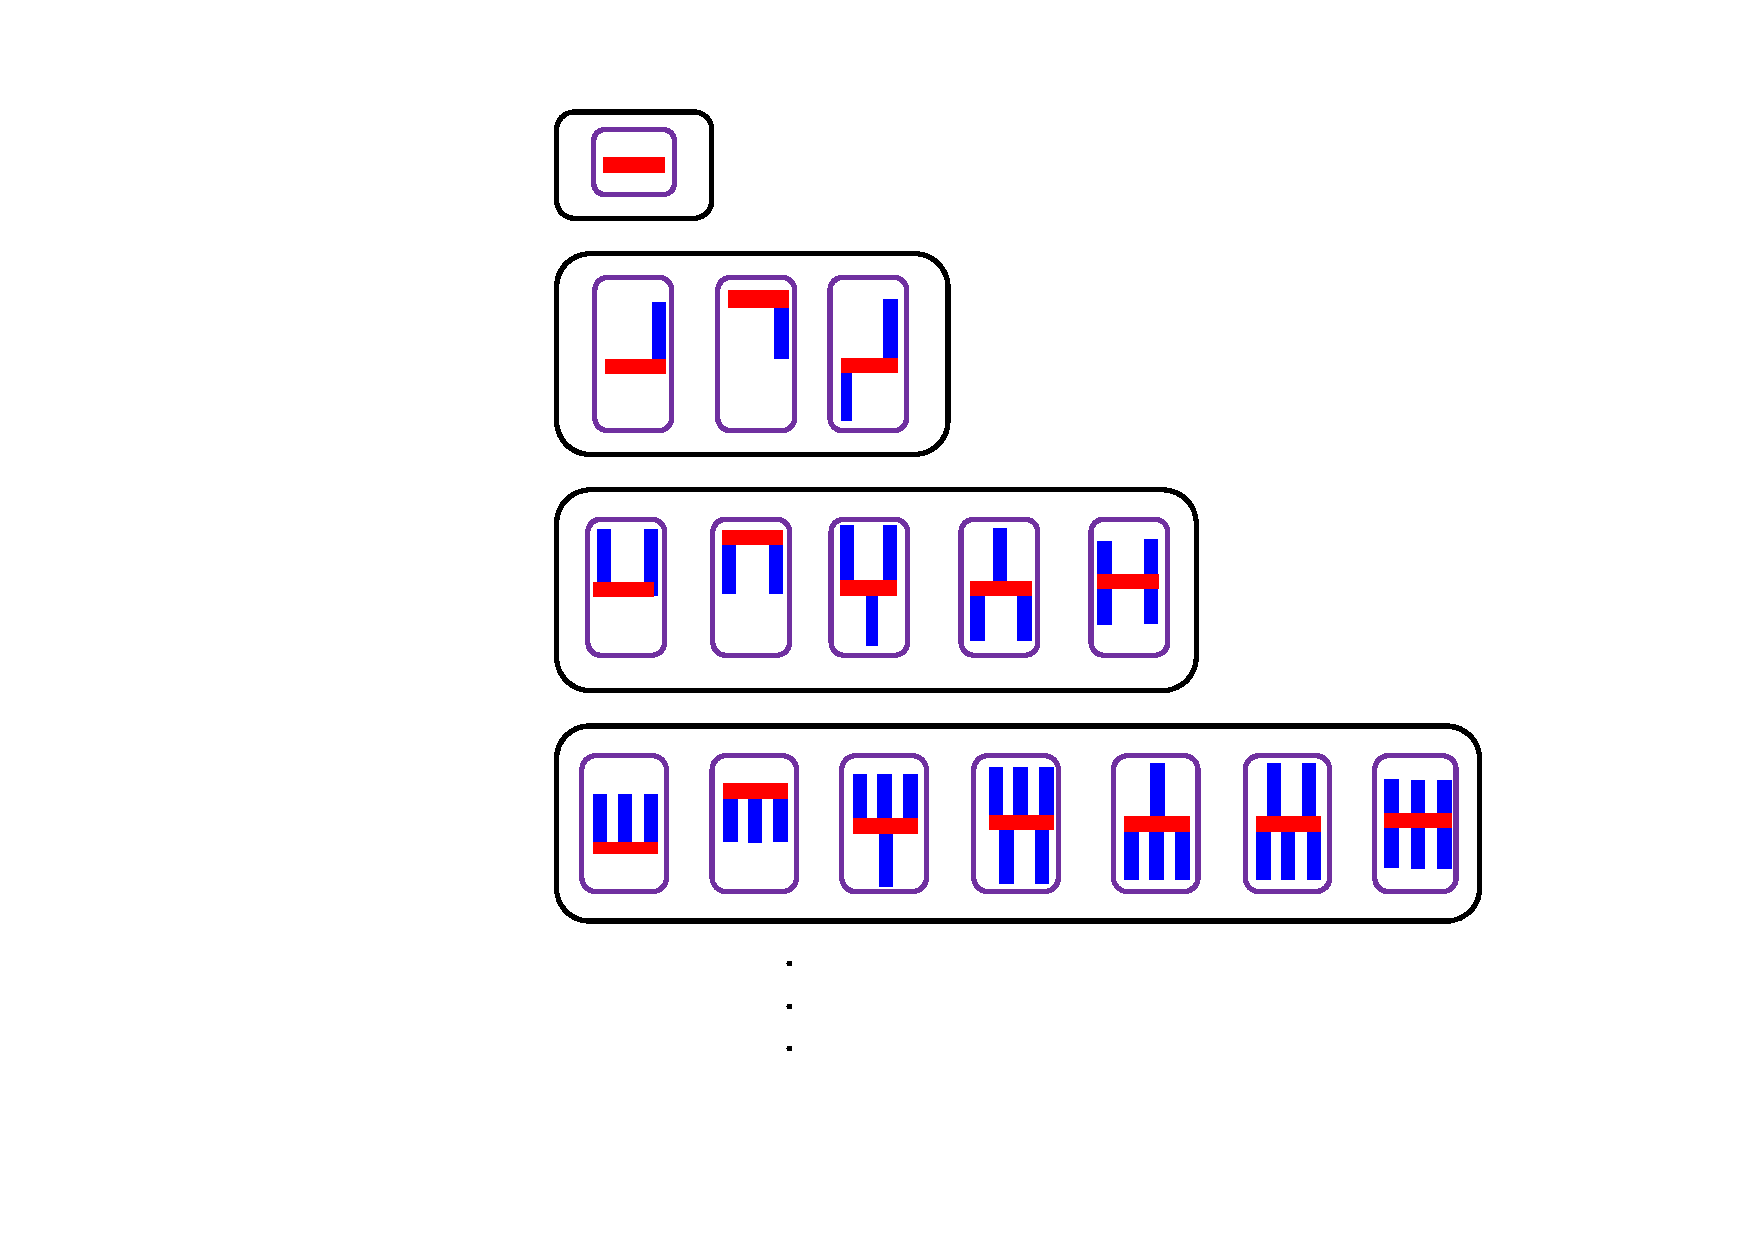
\includegraphics[width=11cm]{Fig/lemma2_1.pdf}
    %\centerline{\psfig{figure=Fig/lemma2_1.eps, width=11cm}}
     \caption{
      \small
       The original bus topology.
   }
  \label{fig::lemma2_1}
\end{figure}

\begin{figure}[htb]
  \centering
    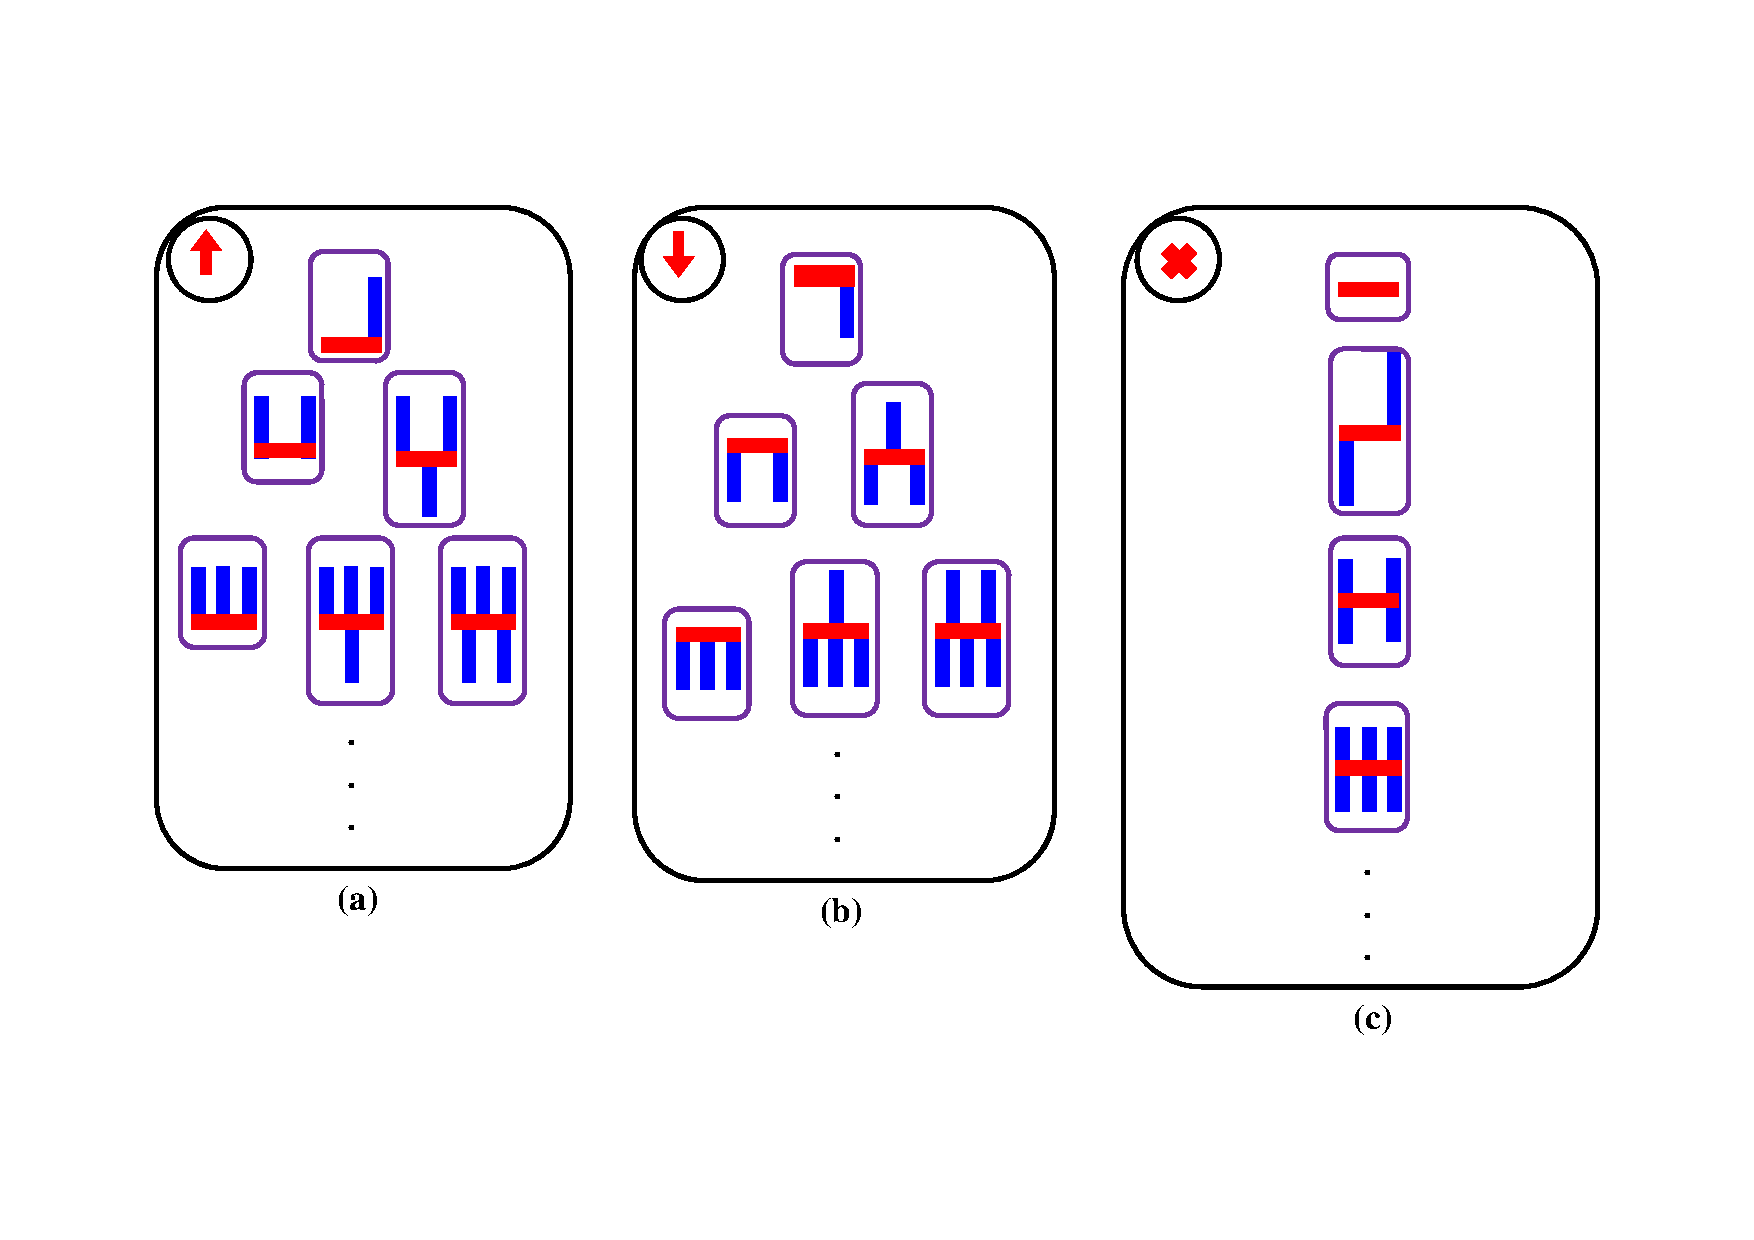
\includegraphics[width=14cm]{Fig/lemma2_2.pdf}
    %\centerline{\psfig{figure=Fig/lemma2_2.eps, width=14cm}}
     \caption{
      \small
       The rules for wirelength reduction.
   }
  \label{fig::lemma2_2}
\end{figure}

Figure~\ref{fig::lemma2_1} and Figure~\ref{fig::lemma2_2} illustrate how to modify the coordinate of each bus component.
In this paper, we explore all possible connective situations between different horizontal and vertical
bus components, parts of the possible connective situations are shown in Figure~\ref{fig::lemma2_1}. In the first row,
there is no any vertical bus components intersecting with the horizontal bus component on both sides.
In the second row, one vertical bus component intersects with the horizontal bus component on one side and one
vertical bus component at most intersects with the horizontal bus component on the other side.
In the third row, two vertical bus components intersect with the horizontal bus component on one side and two
vertical bus components at most intersect with the horizontal bus component on the other side,
the possible situations in other rows can be derived similarly.
All the above situations in Figure~\ref{fig::lemma2_1} can be categorized into three cases as follows:\\
\indent $Case1$: the number of intersecting vertical bus components on upper side of the horizontal bus component
are more than on lower side as shown in Figure~\ref{fig::lemma2_2} (a), thus, the total bus wirelength
will be improved by moving the horizontal bus component toward the upper side.\\
\indent $Case2$: the number of intersecting vertical bus components on lower side of the horizontal bus component
are more than on upper side as shown in Figure~\ref{fig::lemma2_2} (b), thus, the total bus wirelength
will be optimized by moving the horizontal bus component toward the lower side.\\
\indent $Case3$: the number of intersecting vertical bus components are equal on both sides of the horizontal bus component
as shown in Figure~\ref{fig::lemma2_2} (c). No matter how the coordinate of the horizontal bus component is adjusted,
the total bus wirelength remains unchanged.\\

Therefore, each time one horizontal bus component is given, the best bus position can be determined by the
intersecting condition between the horizontal and vertical bus components. For any vertical bus components, the rule can be derived similarly.

\section{Layer Assignment} \label{sec::Layer Assignment}
In this paper, we explore the diagonal connection
that makes the bus shape more flexible to increase the success rate.
Since extra vias are \textbf{\textit{forbidden}} at the bend of the diagonal
buses, we develop an algorithm based on the graph coloring
algorithm to assign the components of the diagonal buses to the
same layer. However, graph coloring is computationally hard. It is
an NP-complete problem if a given graph admits a k-coloring for k
$>=$ 3. In our formulation, it only reserves two layers for bus
routing, then the layer assignment becomes 2-coloring problem and
it can be solved in polynomial time. To obtain the overlapped
information between the horizontal and vertical bus components, it first
constructs the conflict graph by comparing the boundary and
coordinate of each bus component. Each bus component is represented as a node in the
graph, and the edges indicate two bus components are overlapped with each other.
For minimizing the conflict between different bus components, it chooses the node that
has the maximum degree to assign it to layer one, and all its
neighbors in the graph are assigned to layer two. Then it
continues another iteration by selecting one of the neighbors as
the starting point. All the neighbors of the new starting point
are assigned to the opposite layer. The above steps are repeated
until all bus components are assigned to one of the two layers. If odd
cycle occurs in the conflict graph, it means that some neighbors can
not be assigned to the opposite layer of the starting point, then one
of the buses is regarded as infeasible.

\begin{figure}[htb]
  \centering
    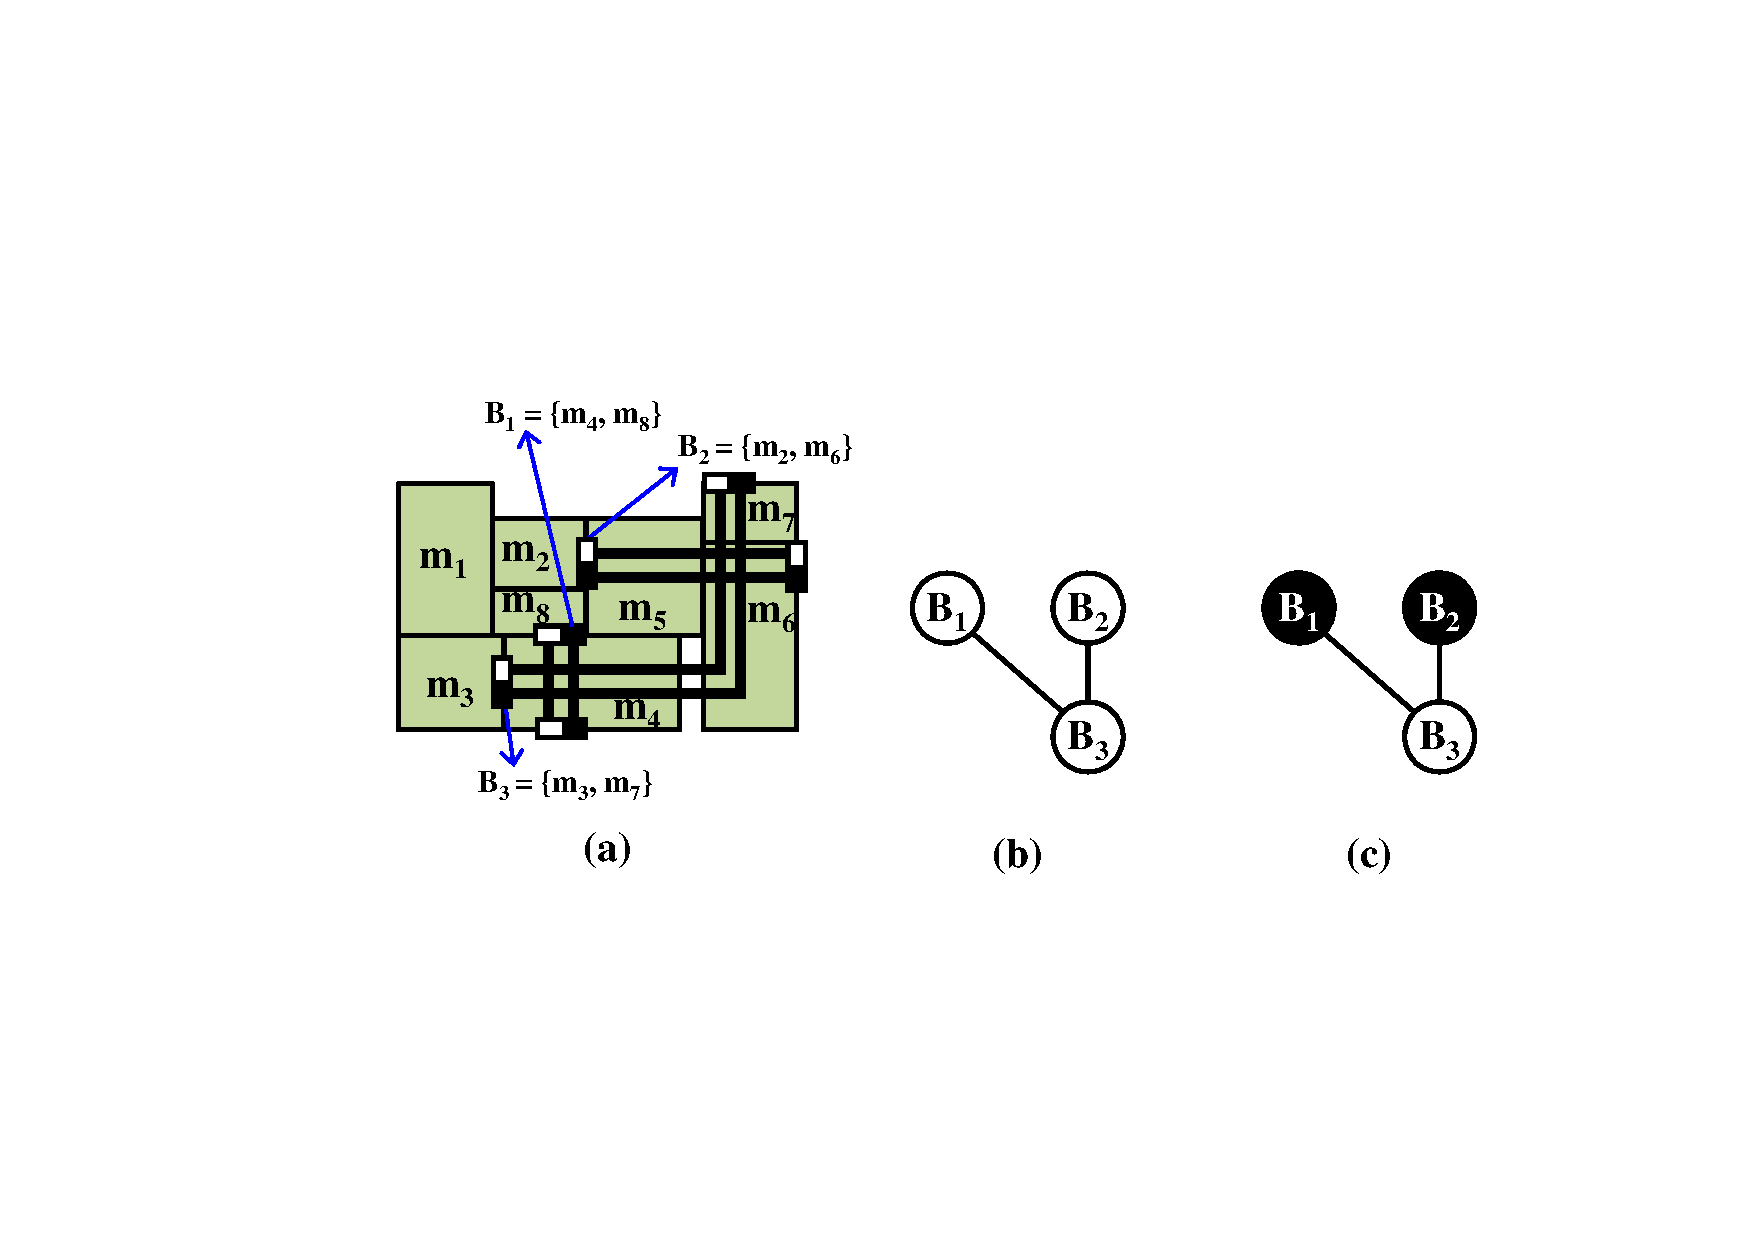
\includegraphics[width=11cm]{Fig/layer_assignment.pdf}
    %\centerline{\psfig{figure=Fig/layer_assignment.eps, width=11cm}}
     \caption{
      Layer assignment.
   }
  \label{fig::layer_assignment}
\end{figure}

Figure~\ref{fig::layer_assignment} illustrates how the
algorithm works. In Figure~\ref{fig::layer_assignment}
(a), there are three buses and the modules passed by those
buses are shown in the brace. The conflict graph is given in
Figure~\ref{fig::layer_assignment} (b).
Due to the bend of diagonal bus $B_3$ occurs at the module which is
not a bus module, it must assign the bus components of the bus $B_3$
to the same layer. Thus, the diagonal bus $B_3$ is represented as the node $B_3$ in the graph.
Initially, the node $B_3$ has the maximum degree in the conflict graph.
We assign it to layer one, and all its neighbors $B_1$ and $B_2$ are assigned
to layer two. Then it terminates because all buses are assigned to one of the two layers.
Figure~\ref{fig::layer_assignment}(c) is the result of layer
assignment, the nodes in layer one are marked with white color,
and the nodes in layer two are marked with black color.

\section{Orientation Determination
and Deviation Minimization}
\label{sec::Orientation Determination}
\subsection{Deviation Minimization with Lookup Table Method}
\label{sec::Deviation Minimization with Lookup Table Method}
%deviation optimization
\begin{figure}[htb]
  \centering
    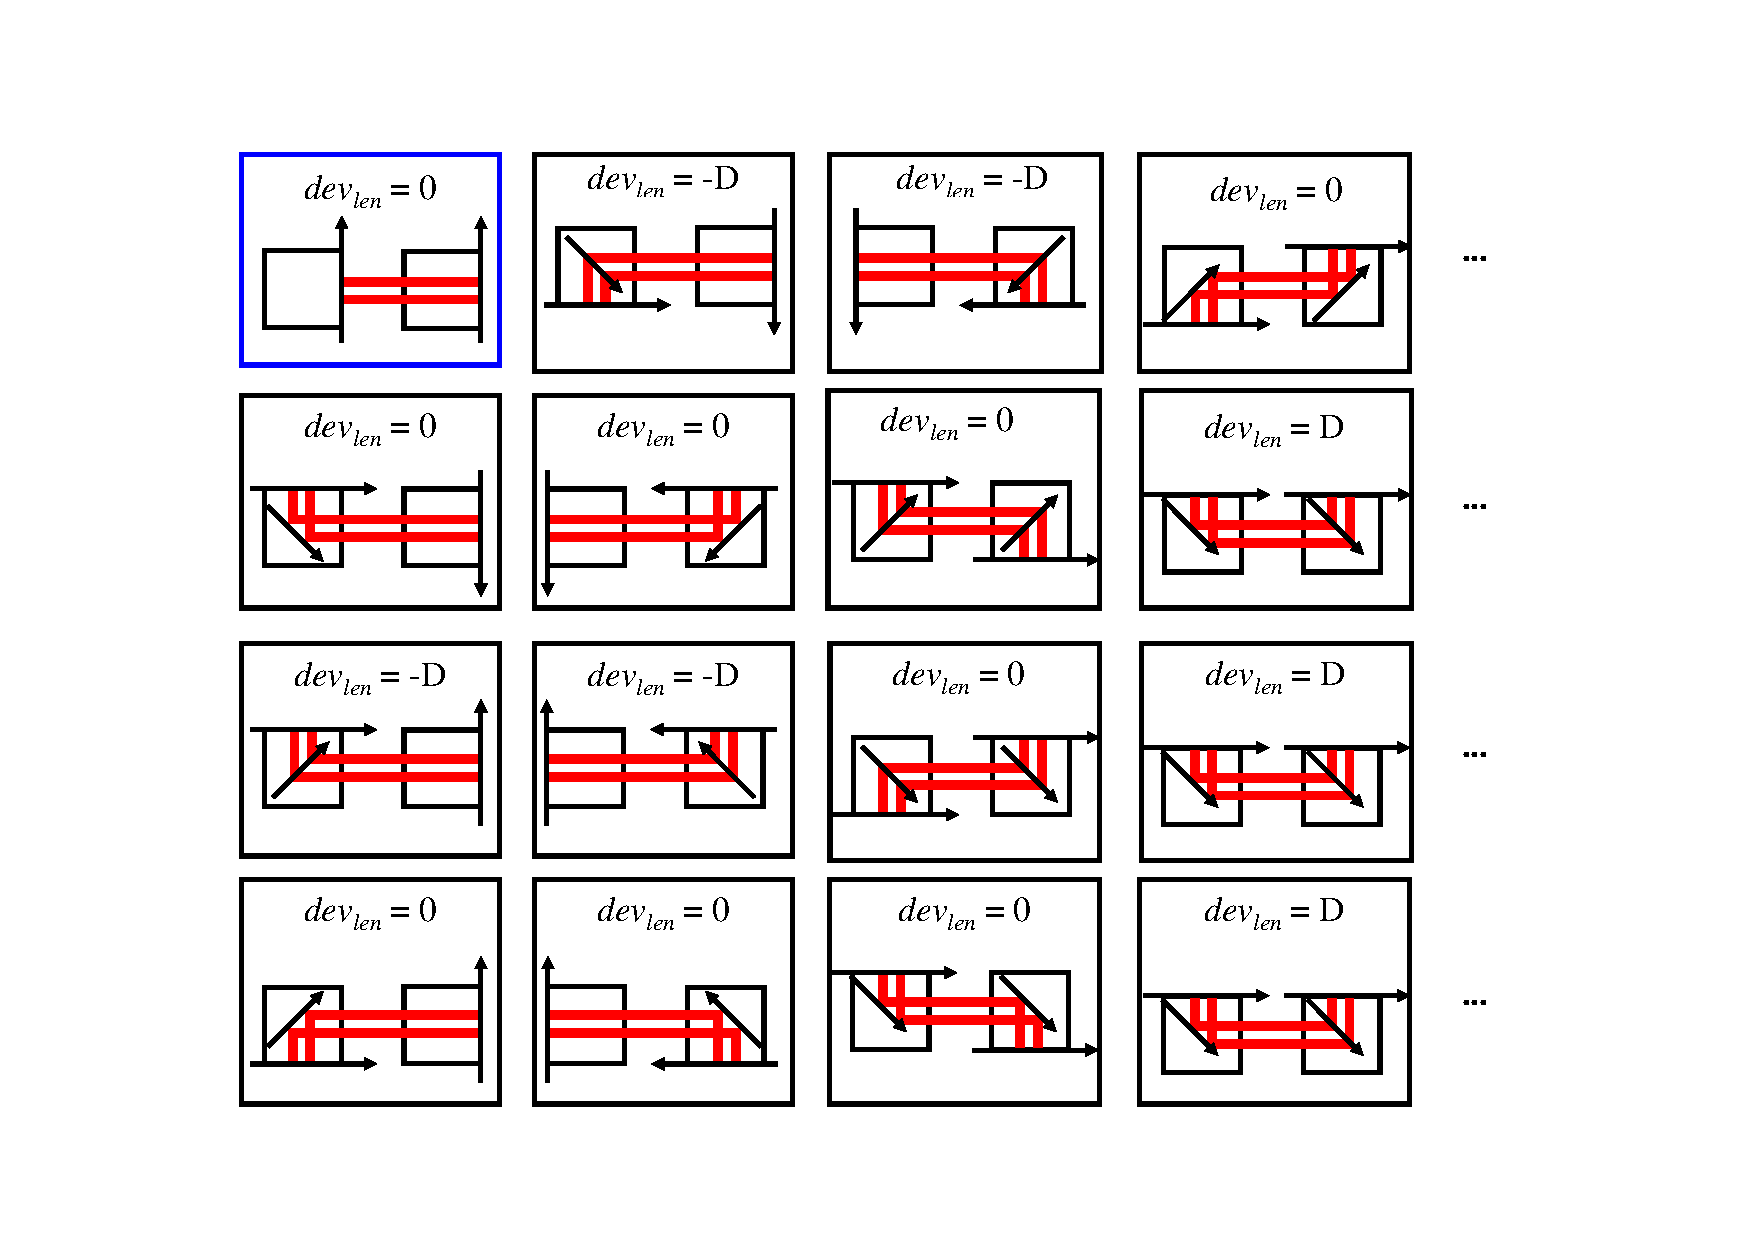
\includegraphics[width=12cm]{Fig/total_deviation_pattern.pdf}
    %\centerline{\psfig{figure=Fig/total_deviation_pattern.eps, width=12cm}
     \caption{
      Total possible bus shapes between any two modules.
   }
  \label{fig::total_deviation_pattern}
\end{figure}

The bus routing problem has attracted much attention recently, and
one of the popular problems is to determine the bus orientation
and minimize the deviation at each load \cite {Mo07_1, Mo07_2}.
However, these works mainly consider the impact of the blockages
during bus routing that have different objective with ours.
Besides, extra vias at the bend of each diagonal bus component
is allowed in the above works, however, the vias have adverse
effects on the bus delay, it is \textbf{\textit{forbidden}} under
our problem formulation.
Therefore, we develop a new algorithm that can be integrated into
our bus-driven floorplanner.

\begin{figure}[htb]
  \centering
    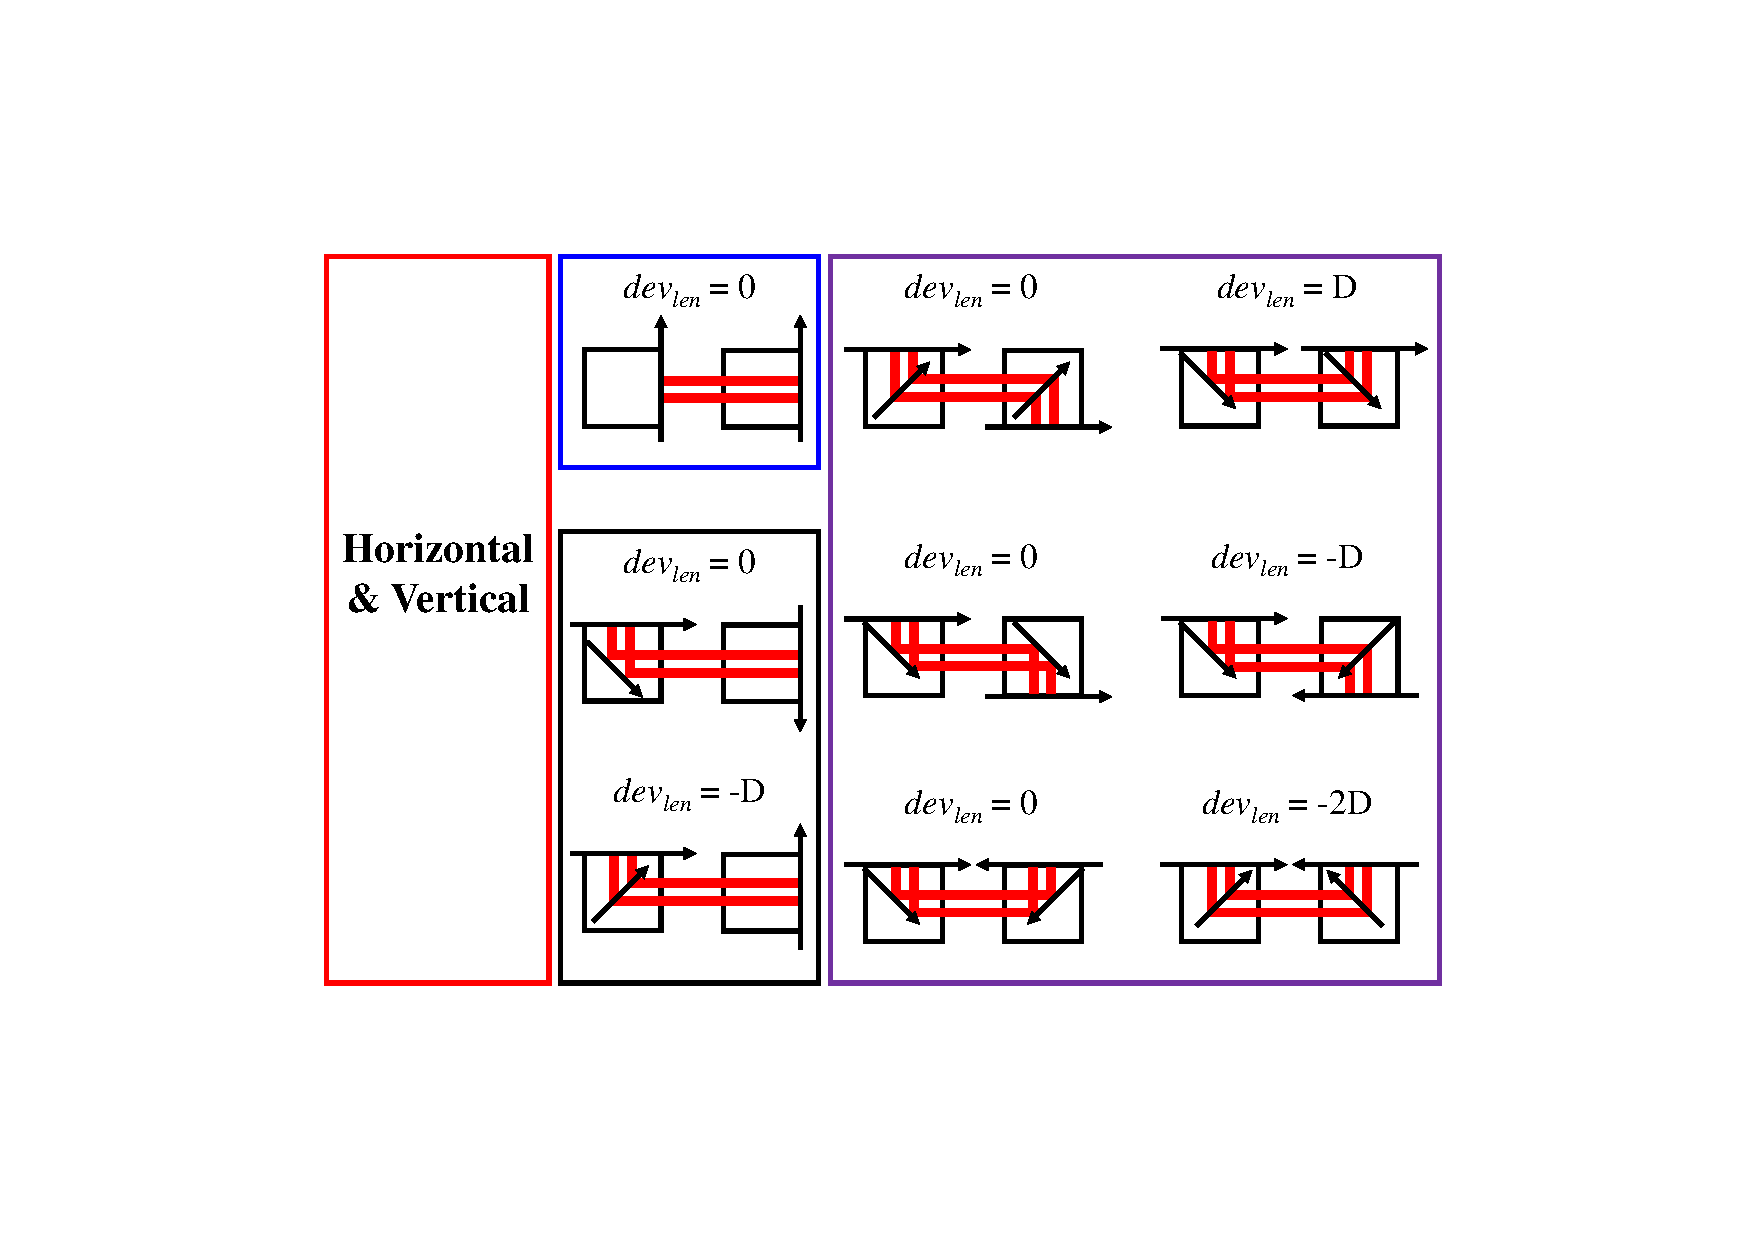
\includegraphics[width=9cm]{Fig/deviation_pattern1.pdf}
    %\centerline{\psfig{figure=Fig/deviation_pattern1.eps, width=10cm}}
  \centering
    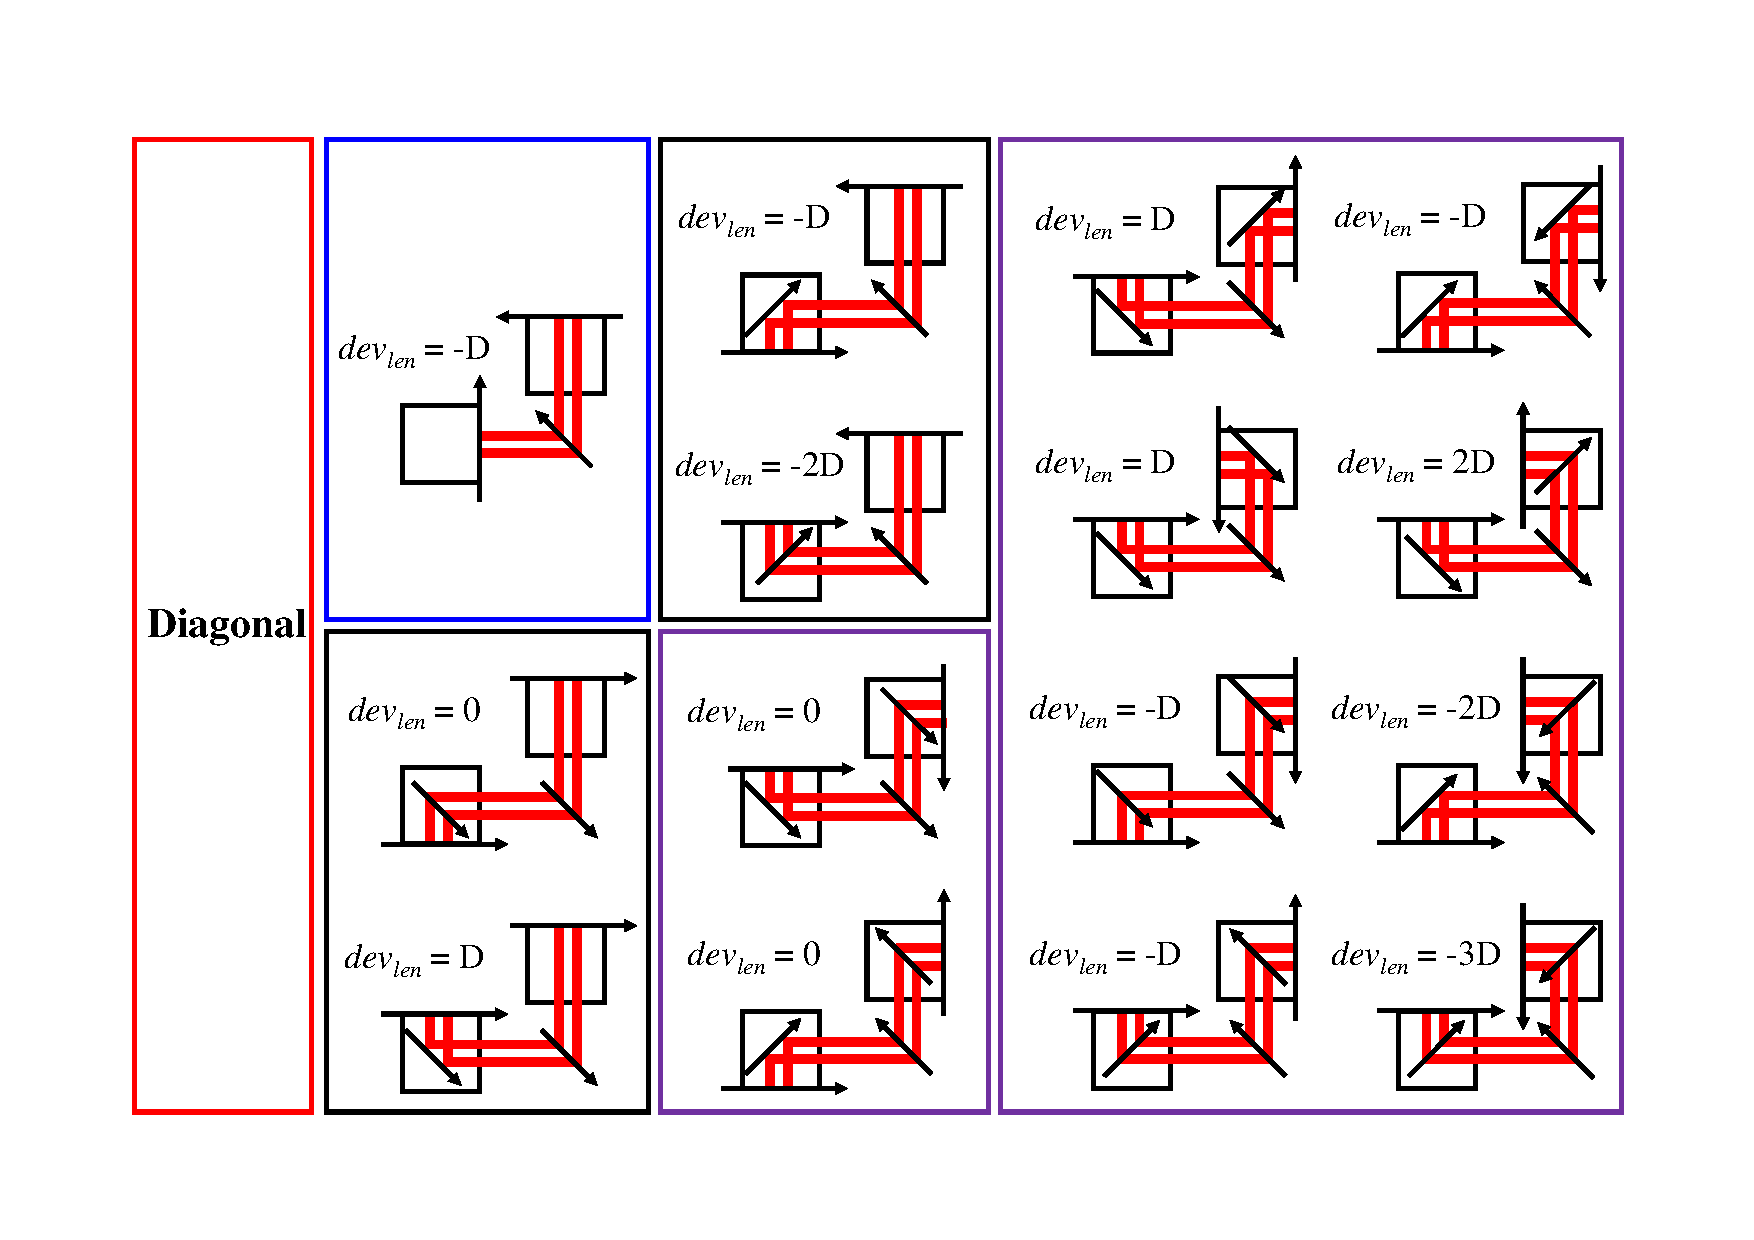
\includegraphics[width=12cm]{Fig/deviation_pattern2.pdf}
    %\centerline{\psfig{figure=Fig/deviation_pattern2.eps, width=13cm}}
     \caption{
      The bus patterns derived from the horizontal, vertical, and diagonal connections.
   }
  \label{fig::deviation_pattern1}
\end{figure}

In this paper, we explore all possible bus shapes including the position of the bus pin
between any two modules, and obtain total 150 possible bus shapes,
part of the total possible bus shapes are illustrated in Figure~\ref{fig::total_deviation_pattern}.
Different bus shapes can be mapped to some general patterns by mirroring or rotating,
finally, total 24 bus patterns are concluded. Given the initial position
of the bus pins on the modules, it can obtain the possible
patterns. Next, according to the accumulated deviation at previous
module, it chooses the pattern holding the best accumulated
deviation at the module. Finally, the accumulated deviation at the
modules, the orientation and position of the bus pins, and the position of the bus pins
can be determined. Figure~\ref{fig::deviation_pattern1} shows the
24 concluded patterns. The arrows represent the position and
orientation of the bus pins at the turning
nodes and the modules. Different cases can contribute different deviations.

\begin{figure}[htb]
  \centering
    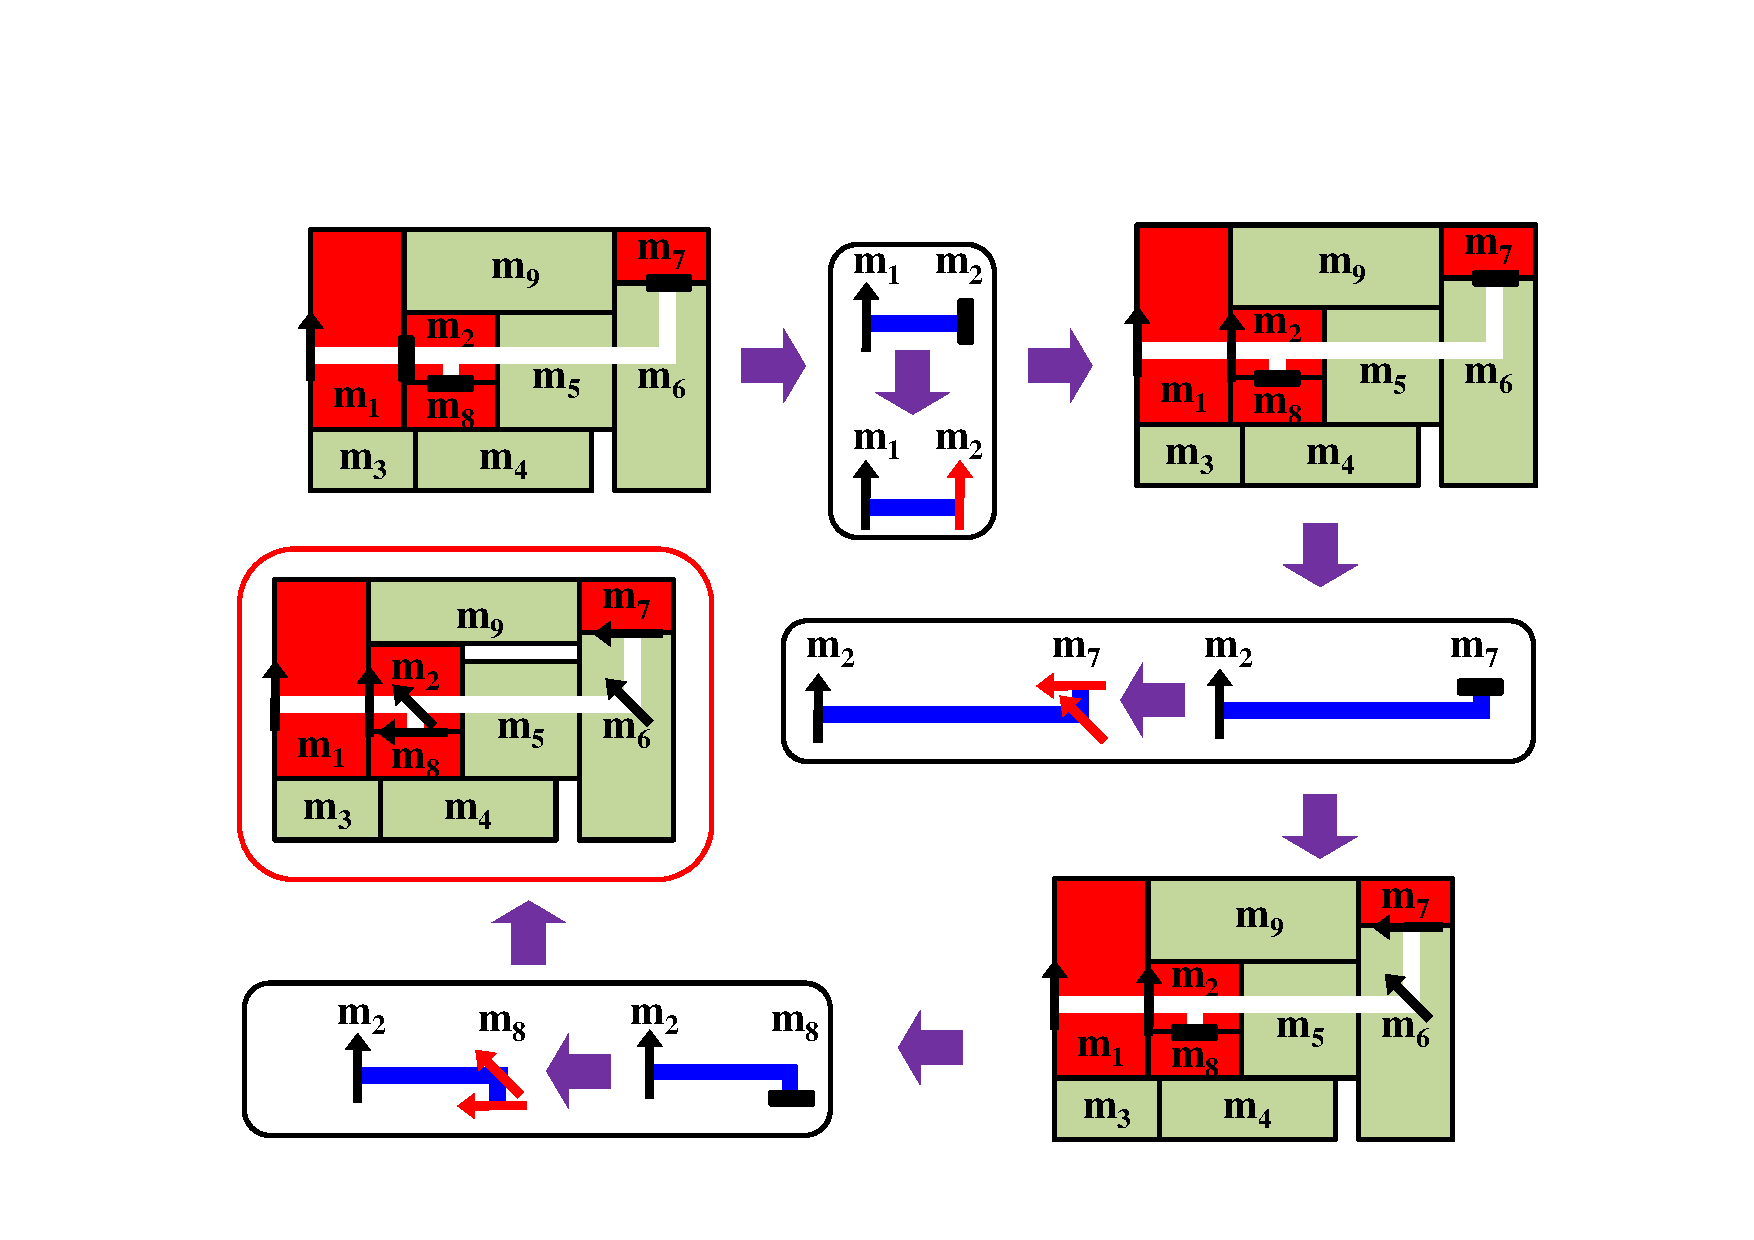
\includegraphics[width=12cm]{Fig/deviation_example1.pdf}
    %\centerline{\psfig{figure=Fig/deviation_example1.eps, width=12cm}}
     \caption{
      Determine the orientation and deviation for all bus pins and turning nodes.
   }
  \label{fig::deviation_example1}
\end{figure}

Figure~\ref{fig::deviation_example1} illustrates how the
algorithm works. There is a bus which passes through the modules in
\{$m_1$, $m_2$, $m_7$, $m_8$\}, each module holds the initial
position of the bus pins, and their orientation is not determined yet.
We assume that $m_1$ is the driver, the searching order obtained from
performing depth first search (DFS) on the MST is $m_1 \rightarrow m_2
\rightarrow m_7 \rightarrow m_8$. The deviation of the driver $m_1$ is 0.
First, the module $m_2$ is picked as the candidate.
The modules $m_1$ and $m_2$ are connected with
a horizontal bus component passing through the bus pins on the modules, so
it can obtain one possible pattern from the 24 concluded patterns.
The obtained pattern contributes 0 at the accumulated deviation, so the
accumulated deviation from the driver to module $m_2$ is still 0, then the
orientation of the bus pin on module $m_2$ is obtained.

Next, the module $m_7$ is chosen as the candidate. The modules $m_2$ and $m_7$
are connected with the diagonal bus component passing through the bus pins on
the modules, so it can obtain one possible pattern from the
24 concluded patterns. The obtained pattern contributes $-$D at the
accumulated deviation, so the accumulated deviation from the
driver to the module $m_7$ is $-$D, then the orientations of the bus
pin on the module $m_7$ and the turning node are obtained.

Finally, the module $m_8$ is selected as the candidate. The modules $m_2$
and $m_8$ are connected with only one vertical bus component. However, the
bus pin on the module $m_2$ is not passed by the
vertical bus component, so it can obtain two possible patterns from the
24 concluded patterns. One pattern contributes 0 at the
accumulated deviation of the module, and another pattern contributed $-$D at the
accumulated deviation of the module. Since the accumulated deviation from the
driver to the previous module $m_2$ is 0, the pattern contributing
0 at the accumulated deviation of the module is chosen. Then the accumulated
deviation from the driver to the module $m_8$ is 0, the orientations of
the bus pin on the module $m_8$ and the turning
node are obtained.
Now the algorithm terminates because the
position and orientation of all bus pins are determined.

\subsection{Fast Deviation Update Based on Topology Comparison}
\label{sec::Fast Deviation Update Based on Topology Comparison}

To decrease the time for searching possible patterns, we propose another approach
which divides the procedure of determining the deviation of each
module into two steps --- deviation determination and accumulated deviation (AD) update.
In each iteration, the AD can be quickly updated after the deviation of the candidate is determined.
Since the process of determining the deviation of each
module is split, the shorter segment is needed for each comparison during searching the best pattern.
If the bus pin on different modules can be connected by one straight line, then its deviation is equal to its AD,
therefore, and those bus patterns are unnecessary kept in the concluded bus patterns.
Finally, total 24 bus patterns can be further reduced to 10 types.
\begin{figure}[htb]
  \centering
    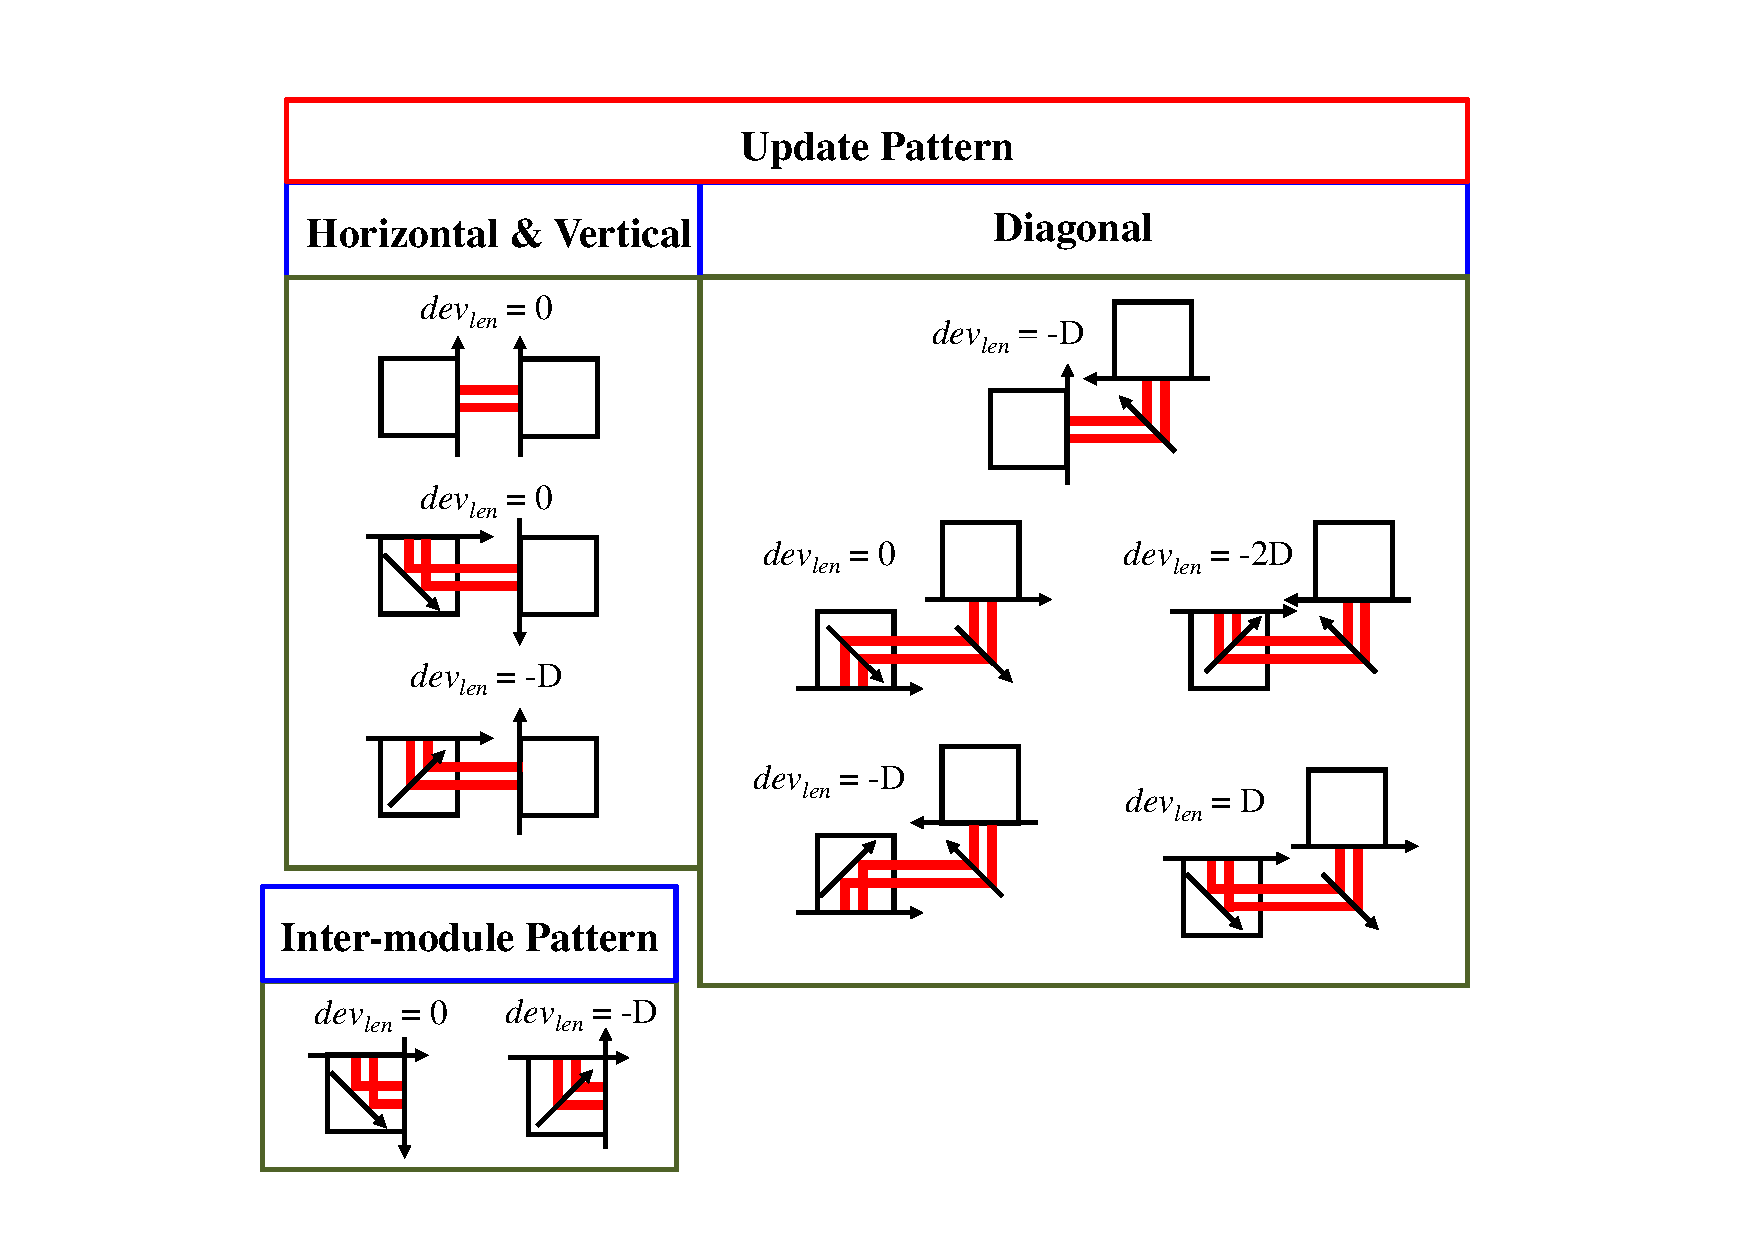
\includegraphics[width=11cm]{Fig/deviation_reduced_pattern.pdf}
    %\centerline{\psfig{figure=Fig/deviation_reduced_pattern.eps, width=11cm}}
     \caption{
      The reduced bus patterns.
   }
  \label{fig::deviation_reduced_pattern}
\end{figure}

Figure~\ref{fig::deviation_reduced_pattern} gives total 10 concluded
bus patterns. The deviation of each candidate is determined from the inter-module patterns, and the update patterns
are used to update the AD of its neighbors.
In this algorithm, the candidate is chosen based on the searching order which is obtained by performing
breadth first search (BDF) on the MST, if a module has at least two neighbors, the neighbors are selected clockwise from its upper side.

\begin{figure}[htb]
  \centering
    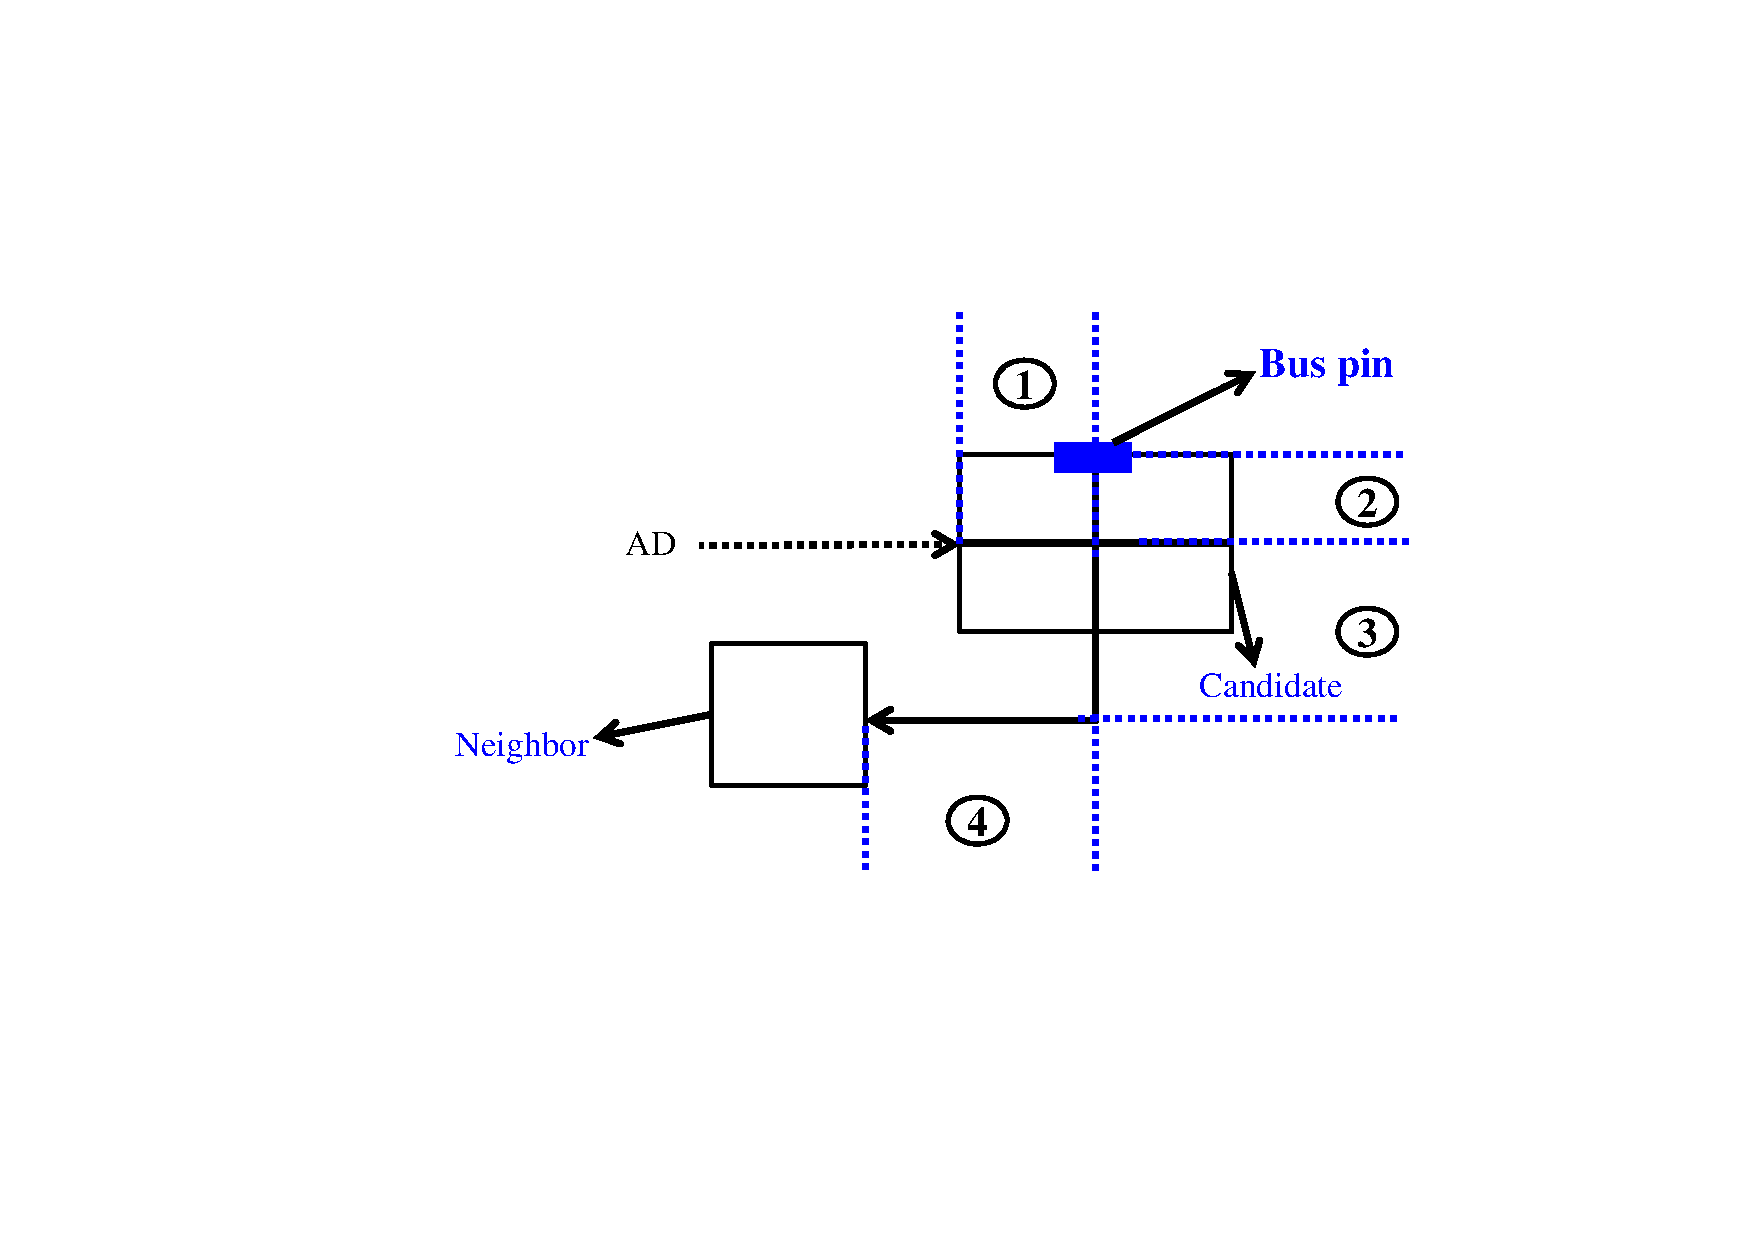
\includegraphics[width=11cm]{Fig/deviation_calculation.pdf}
    %\centerline{\psfig{figure=Fig/deviation_calculation.eps, width=11cm}}
     \caption{
      The procedure of deviation determination and AD update.
   }
  \label{fig::deviation_calculation}
\end{figure}

Figure~\ref{fig::deviation_calculation} shows how the algorithm works.
Initially, the bus pin of the candidate is placed on its upper boundary.
Based on different AD on the module, the best deviation and orientation can be obtained from the inter-module patterns.
We assume that the best deviation can be obtained at the candidate if the bus pin is placed on its upper boundary,
then segment 1 and segment 2 are chosen to determine the deviation at the candidate.
According to different relative positions between the candidate and its neighbors,
it finds the matched pattern with segment 1, segment 3, and segment4 from the update patterns,
then the AD of its neighbors can be obtained.

\begin{figure}[htb]
  \centering
    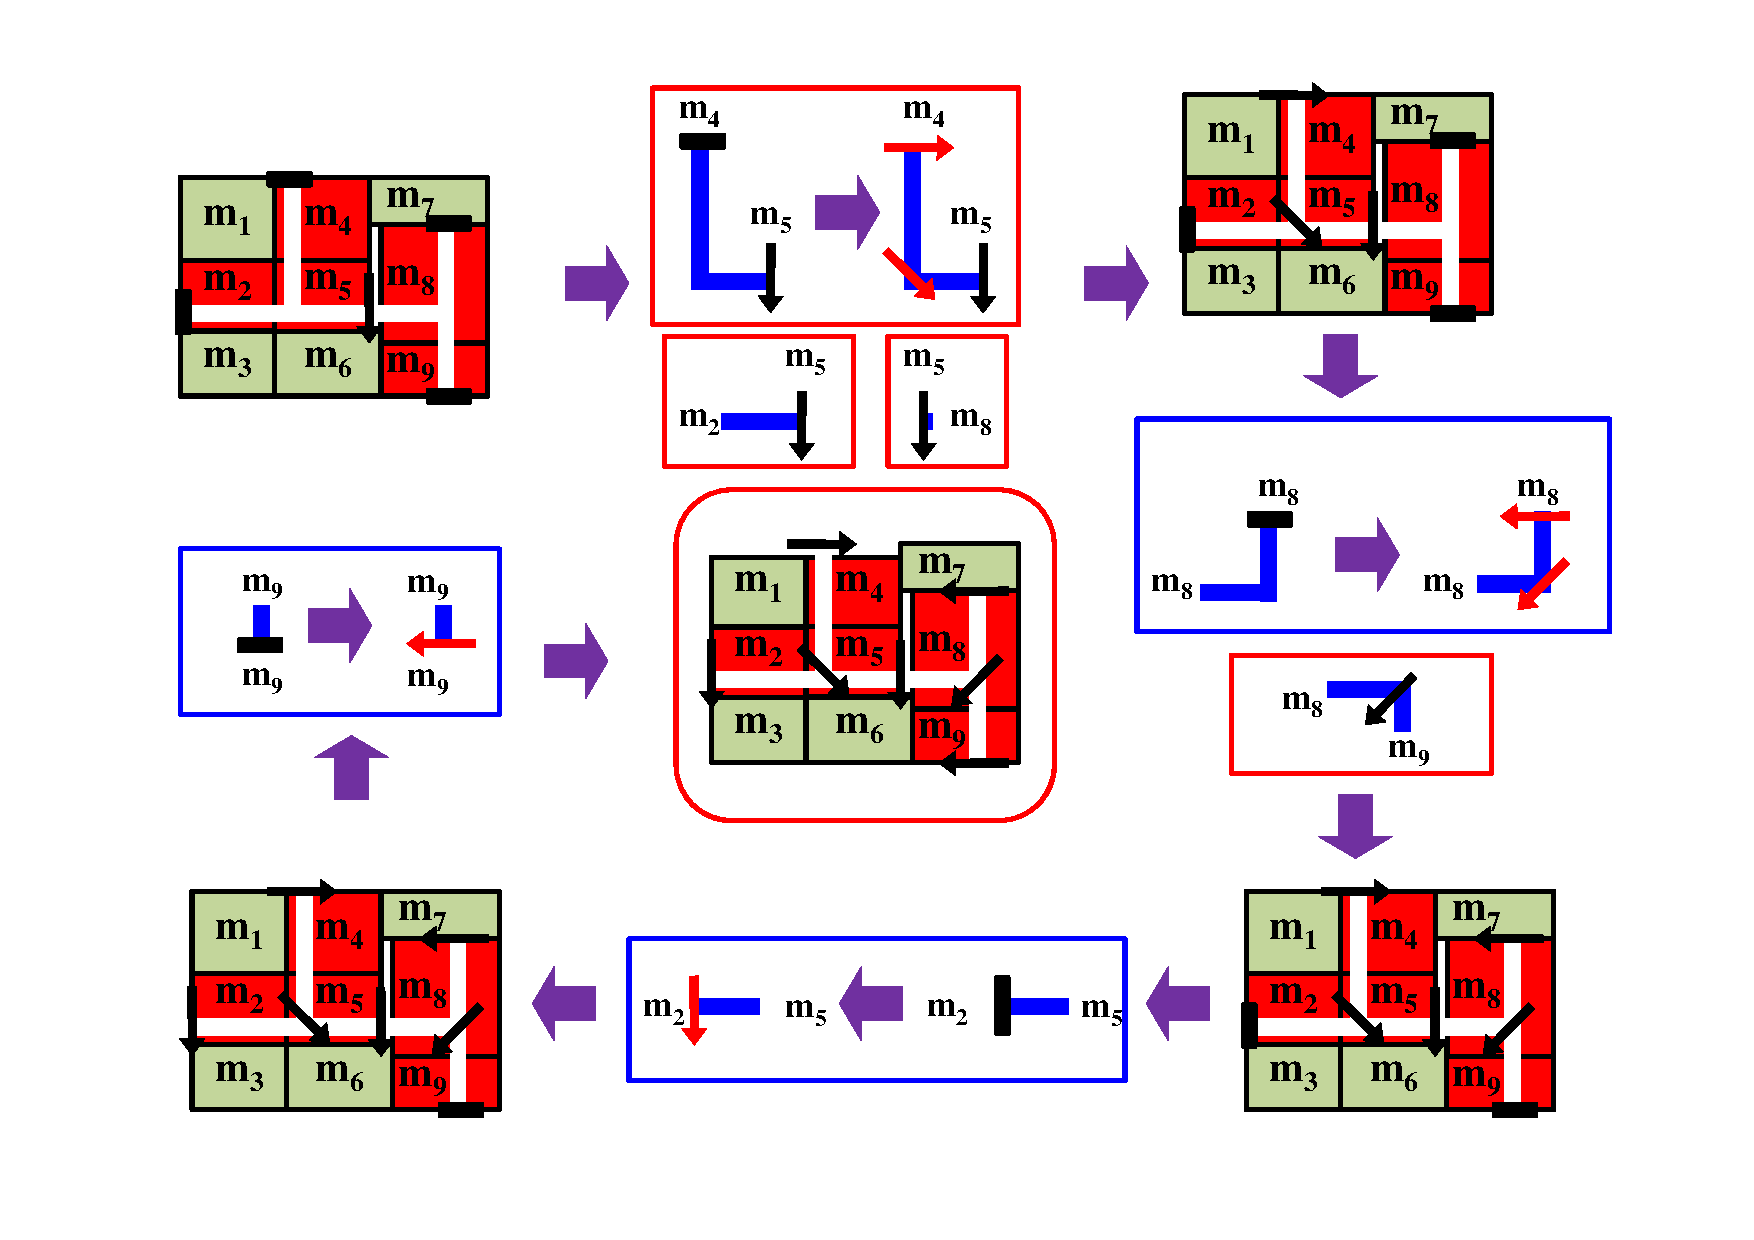
\includegraphics[width=13cm]{Fig/deviation_example2.pdf}
    %\centerline{\psfig{figure=Fig/deviation_example2.eps, width=13cm}}
     \caption{
      Determine the orientation and deviation for all bus pins and turning nodes.
   }
  \label{fig::deviation_example2}
\end{figure}

Figure~\ref{fig::deviation_example2} gives an example to illustrate how the algorithm works.
There is a bus which passes through the modules in
\{$m_2$, $m_4$, $m_5$, $m_8$, $m_9$\}, each module holds the initial
position of the bus pins, and their orientation is not determined yet. We assume that $m_5$ is
the driver, the searching order obtained from performing BFS on the MST is $m_5 \rightarrow m_4
\rightarrow m_8 \rightarrow m_2 \rightarrow m_9$. First, the module $m_5$ is
picked as the candidate. Since $m_5$ is the driver, its deviation is 0, then the AD of its neighbors
are updated based on their relative positions.
First, the best pattern from the update patterns is chosen to determine the orientation at the turning nodes in the driver,
then the orientation and position of the bus pin on module $m_4$, the deviation at the module $m_4$ could be obtained.
Next, it updates the AD for the modules $m_8$ and $m_2$. In next iteration, the module $m_4$ is selected as the candidate.
However, the deviation at the module $m_4$ is obtained and it has no neighbor,
the next module in the searching order is chosen to continue the procedure.
In next iteration, the module $m_8$ is selected as the candidate.
It first finds the best pattern from the inter-module patterns to determine its deviation.
Then it updates AD for its neighbors $m_9$. In next iteration, the module $m_2$ is chosen as the candidate.
Since the bus pin on module $m_2$ is connected by only one straight bus line, its deviation is equal to
its AD. Finally, it selects the module $m_9$ as the candidate, the deviation of the module $m_9$ is equal to
its AD because the bus pin is connected by only one straight bus line.
Now the algorithm terminates because the position and orientation of all bus pins are determined.

\begin{figure}[htb]
  \centering
    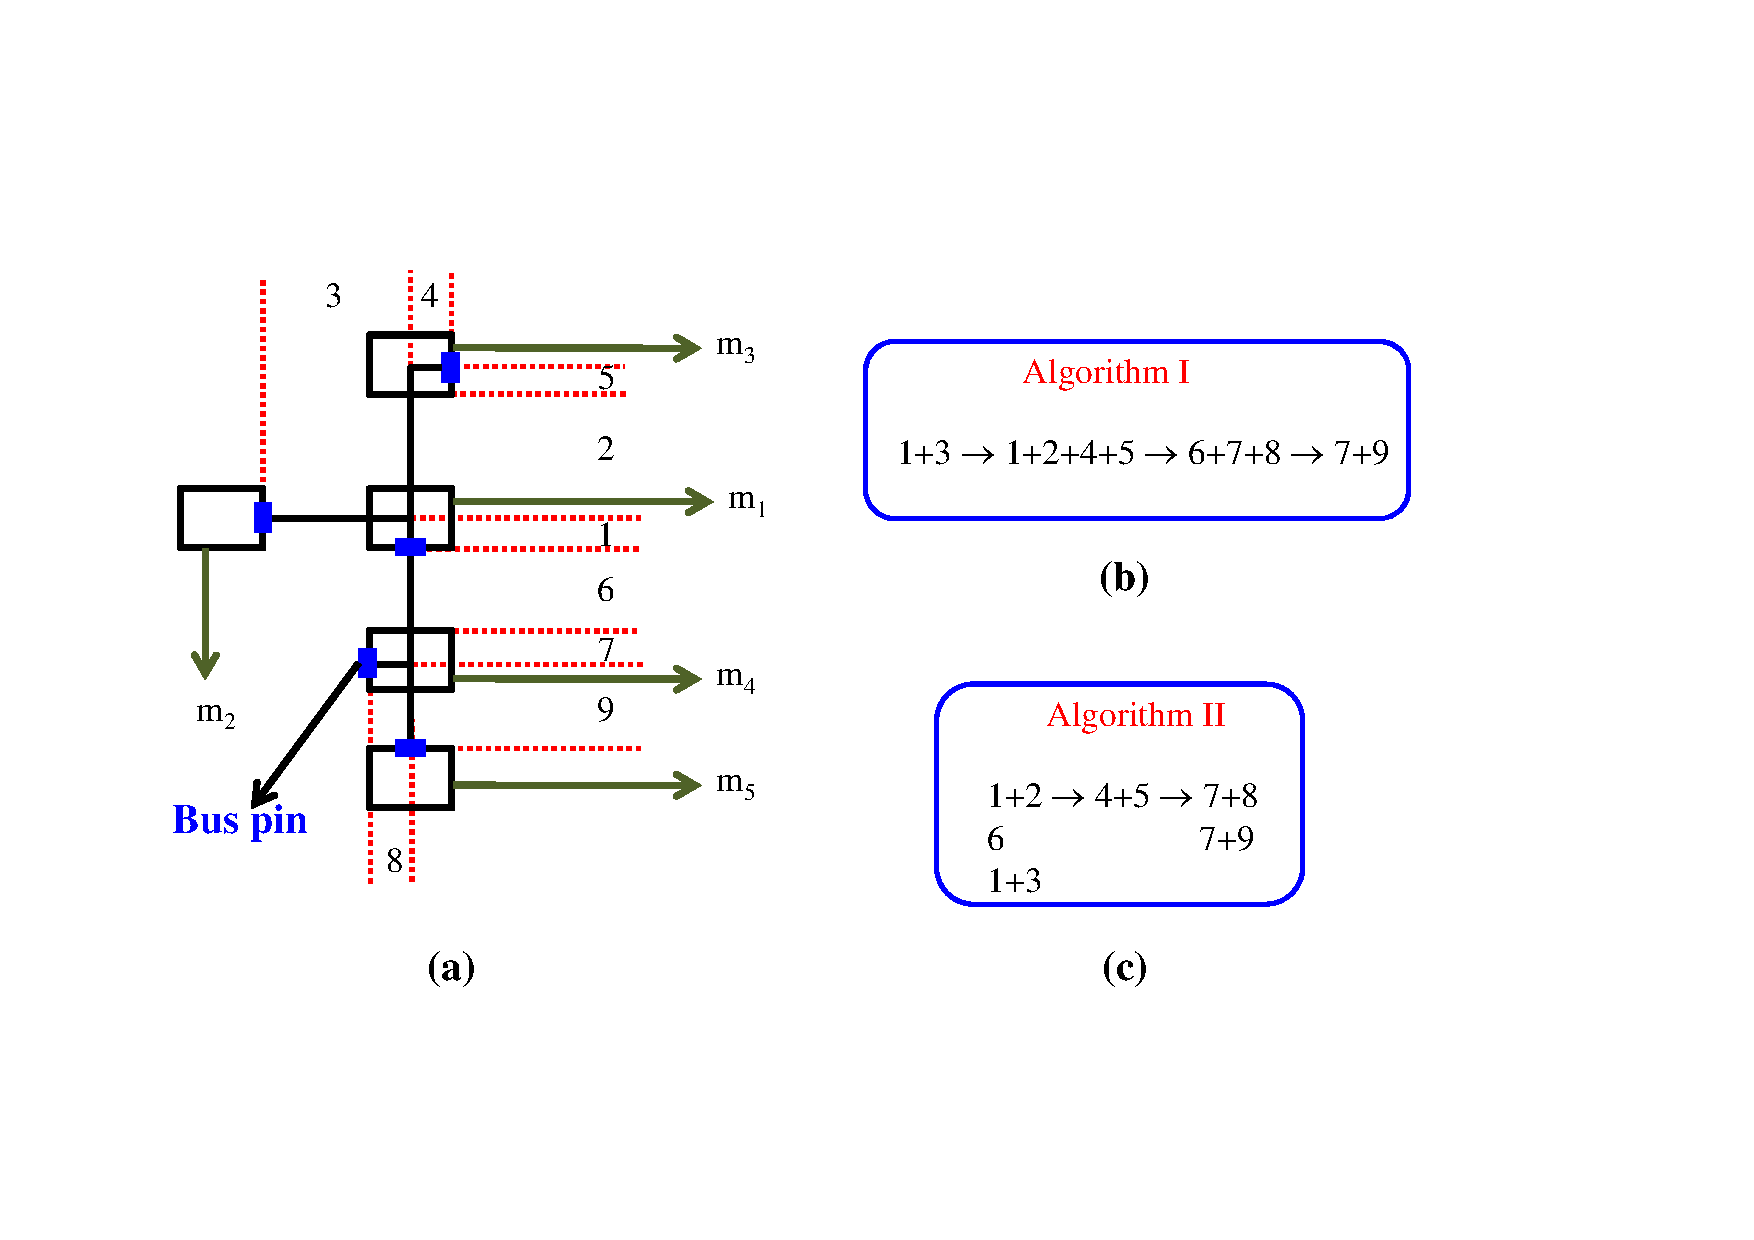
\includegraphics[width=13cm]{Fig/algorithm_comparison.pdf}
    %\centerline{\psfig{figure=Fig/algorithm_comparison.eps, width=13cm}}
     \caption{
      The difference between two algorithms.
   }
  \label{fig::algorithm_comparison}
\end{figure}

We use Figure~\ref{fig::algorithm_comparison} to demonstrate the difference between two algorithms.
In Figure~\ref{fig::algorithm_comparison} (a), there are five modules connected with one bus and each bus segment is marked as a number.
The module $m_1$ is the driver. For the first algorithm, we assume the searching order is $m_1 \rightarrow m_2 \rightarrow m_3 \rightarrow m_4 \rightarrow m_5$,
the sequence of the bus segments which is processed during the algorithm is shown in Figure~\ref{fig::algorithm_comparison} (b).
As for the second algorithm, the searching order is $m_1 \rightarrow m_3 \rightarrow m_4 \rightarrow m_2 \rightarrow m_5$,
the sequence of the bus segments which is processed during the algorithm is shown in Figure~\ref{fig::algorithm_comparison} (c).

As given in Figure~\ref{fig::algorithm_comparison} (b) and Figure~\ref{fig::algorithm_comparison} (c),
it shows that the bus patterns are more complicated in first algorithm than in second algorithm, thus,
the number of the possible bus patterns in first algorithm are more than the number of the possible bus patterns in second algorithm,
and it will spend more time to search for a best pattern.

\begin{Lemma}
For some specific bus topologies in the candidate, the AD of its neighbors can be
directly calculated without searching for the best bus pattern.
\end{Lemma}

\begin{figure}[htb]
  \centering
    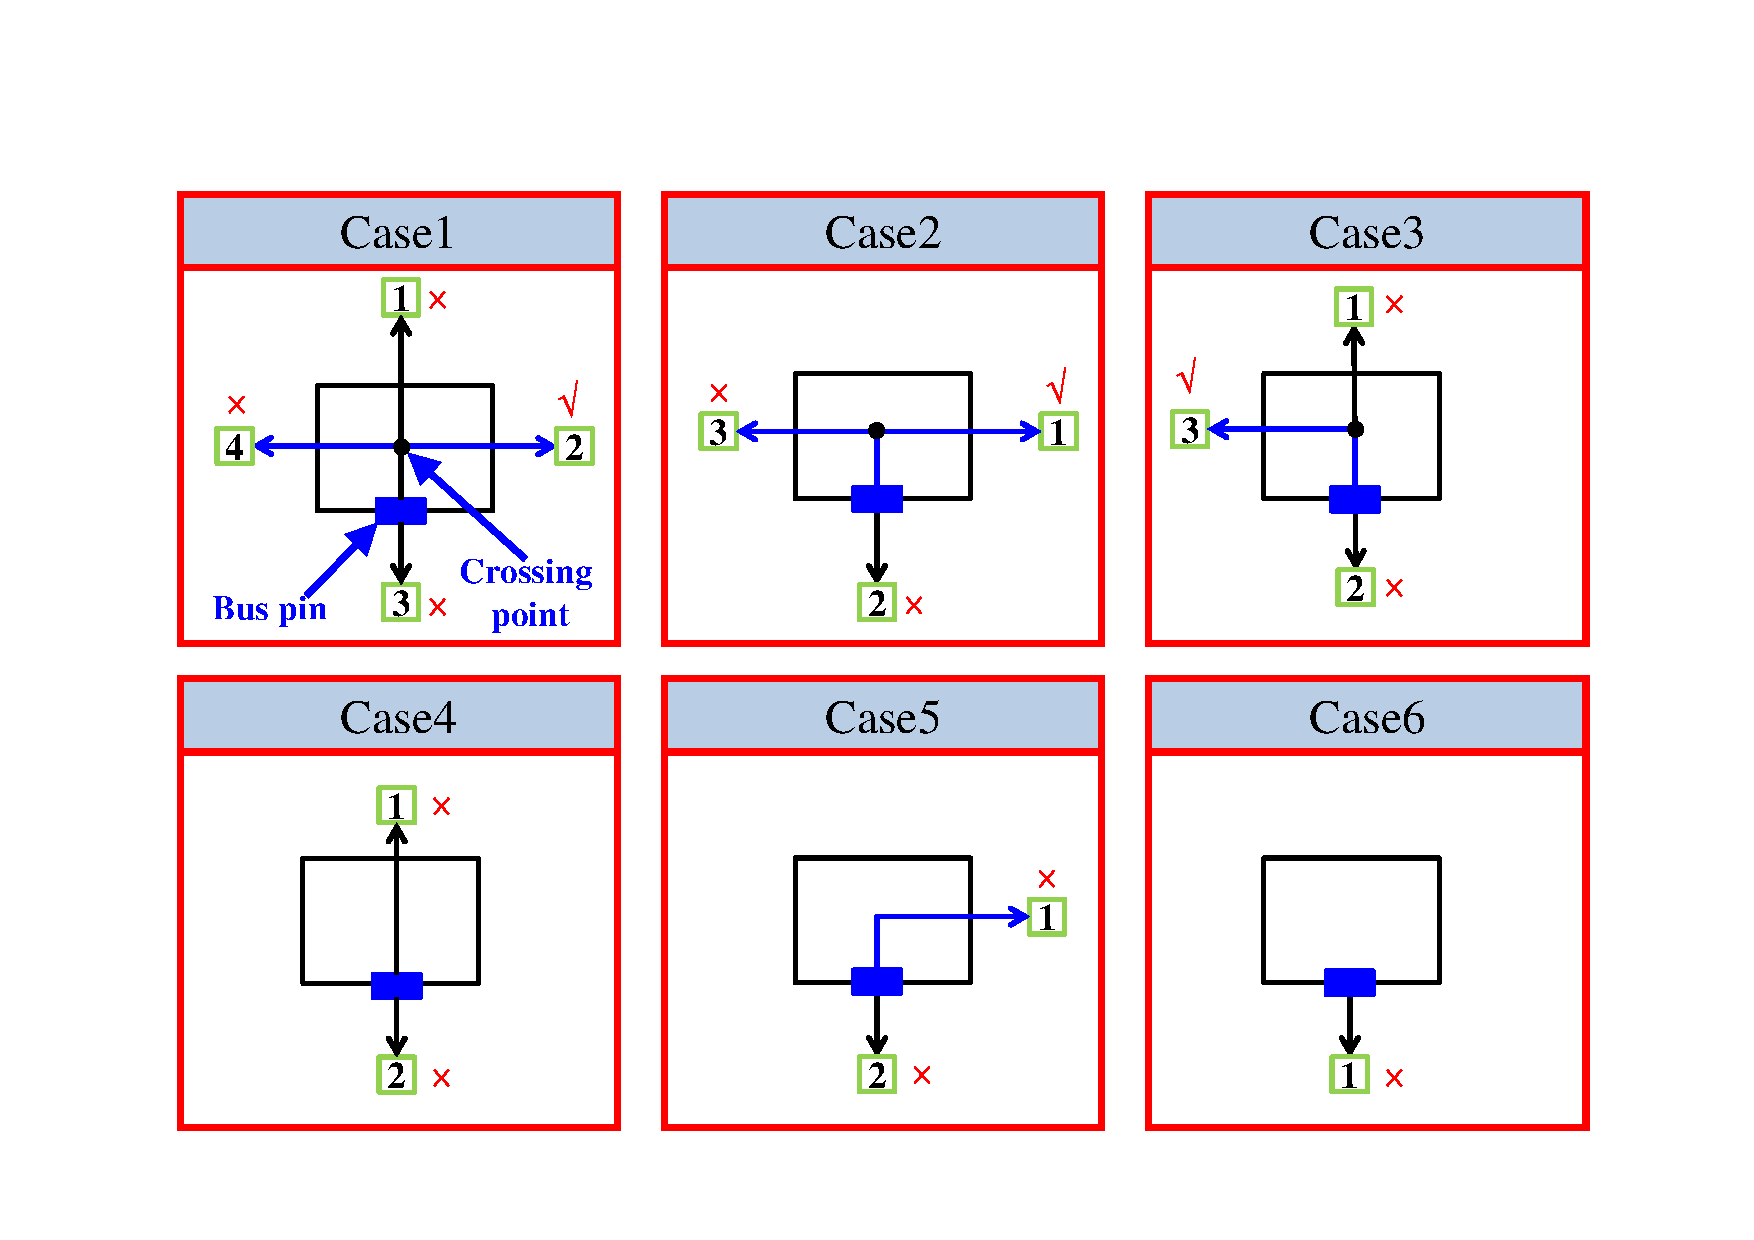
\includegraphics[width=11cm]{Fig/deviation_driver.pdf}
    %\centerline{\psfig{figure=Fig/deviation_driver.eps, width=11cm}}
     \caption{
      All possible topologies in driver.
   }
  \label{fig::deviation_driver}
\end{figure}

In the following, several cases will be analyzed under different conditions.
As shown in Figure~\ref{fig::deviation_driver}, there are total six possible topologies
in the driver, all other topologies can be mapped to these six cases by rotating or mirroring.
In case 1, the driver has four neighbors.
Since the modules at the direction 1 and direction 3 are connected by one straight line to
the bus pin of the driver. There is no deviation contributed by the driver.
The AD of the module at the direction 1 and direction 3 are determined by the relation position between the driver and it.
If the modules at the direction 1 and direction 3 are connected by one diagonal bus with the driver, then it will contribute D or -D to the AD of the module.
The deviation of the modules at the direction 2 will be determined by finding the best
pattern from the update patterns as shown in Figure~\ref{fig::deviation_reduced_pattern},
then the best orientation at the crossing point can be obtained.
Since the orientation at the crossing point have been obtained, the AD of the module at the direction 4
can be calculated based on the orientation at the crossing point
and the relative position between the driver and it.
The directions are attached a tick mark if it needs to search the best bus pattern,
and the directions are attached a cross mark if the AD of the module can be directly calculated.
All other cases can be derived similarly.

Through the above cases, it can get the following conclusion:
since the neighbors of the candidate are processed in the clockwise from the north side,
if the bus pin on the driver is oriented horizontally and the driver has a right neighbor,
then the deviation at the right neighbor is obtained by searching the best pattern from the update patterns,
or the bus pin on the driver is oriented horizontally and the driver has only a left neighbor,
then the deviation at the left neighbor is obtained by searching the best pattern from the update patterns.
However, if the bus pin on the driver is oriented vertically and the driver has a upper neighbor,
then the deviation at the upper neighbor is obtained by searching the best pattern from the update patterns,
or the bus pin on the driver is oriented vertically and the driver has only a lower neighbor,
then the deviation at the lower neighbor is obtained by searching the best pattern from the update patterns.
After obtaining the orientation of the crossing point, the modules at other directions can be directly calculated
based on the obtained orientation and the relative position between the driver and it.

\begin{figure}[htb]
  \centering
    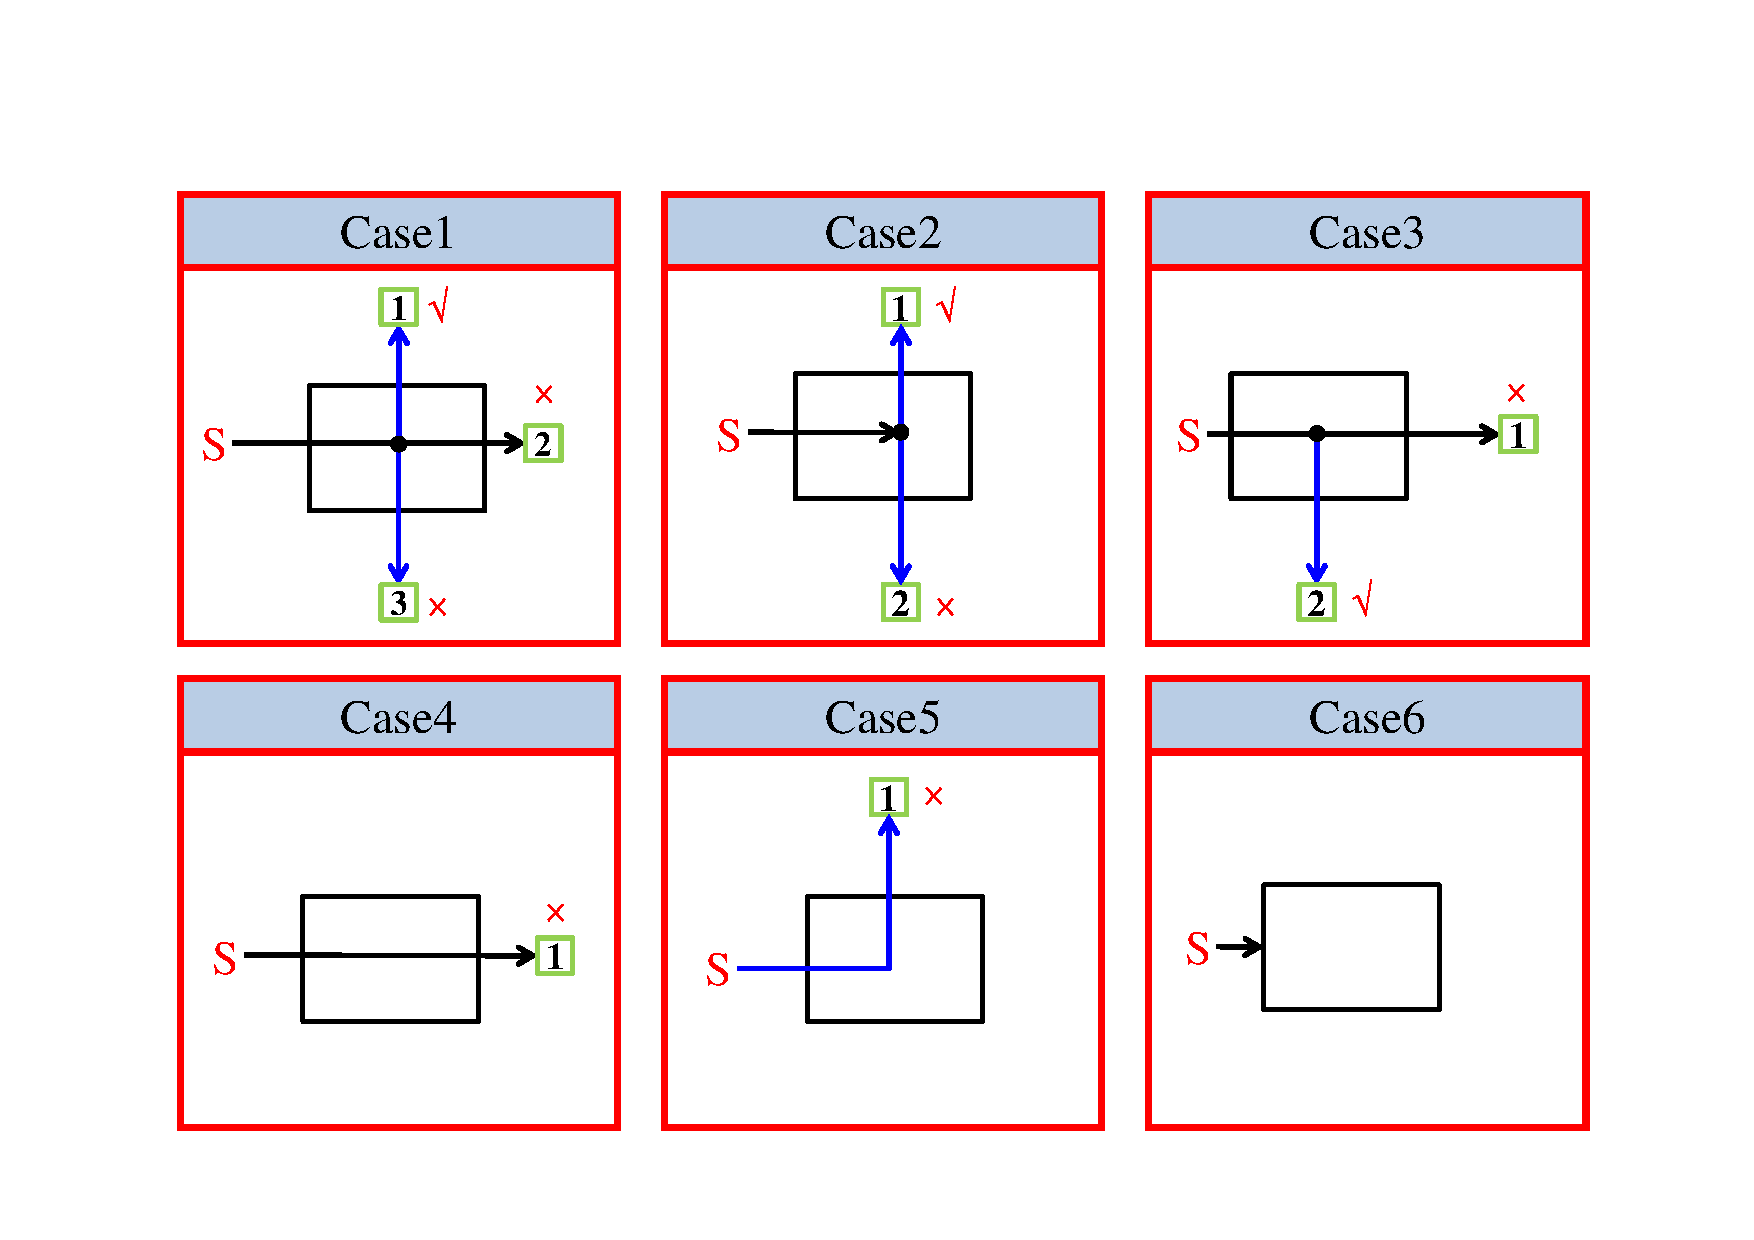
\includegraphics[width=11cm]{Fig/deviation_load.pdf}
    %\centerline{\psfig{figure=Fig/deviation_load.eps, width=11cm}}
     \caption{
      All possible topologies in load.
   }
  \label{fig::deviation_load}
\end{figure}

In Figure~\ref{fig::deviation_load}, there are total six possible topologies
in the load. The $``$\textbf{\textit{S}}$"$ stands for the accumulated direction of the deviation
from the driver.
The rule can be derived in the same way when the candidate is the driver.
If one neighbor of the candidate is at the first orthogonal direction compared with the accumulated direction
and the orientation of the crossing point is still not determined,
then the deviation of the neighbor is obtained by searching the best pattern from the update patterns,
after that, the modules at other directions will be directly calculated based on the obtained orientation and the
relative position between the driver and it.
According to the above rules, it will avoid unnecessary comparison, then the time for searching the best deviation will be minimized.

\section{Soft Module Adjustment} \label{sec::SOFT MODULE ADJUSTMENT}
In order to minimize the chip area, it adjusts the
dimension of some modules such that a better chip area can be
obtained. The adjustment is the same as that in \cite{Xiang03}.
The step is processed with another simulated annealing
process with the same cost function. In
each iteration of the annealing process, it chooses the module
lying on the critical path to change either its width or height a
little bit. However, if any feasible bus become invalid after
the adjustment, the candidate solution will be discarded.


%%%%%%%%%%%%%%%%%%%%%%%%%%
\chapter{Experimental results}
\label{chap::EXPERIMENTAL RESULTS}
%%%%%%%%%%%%%%%%%%%%%%%%%%

\baselineskip=26pt

\section{Experiments on Regular Testcases for \cite{Ma08} and \cite{PH10}}
\label{sec::EXPERIMENTS ON REGULAR TESTCASES}
\begin{figure}[htb]
{
  \centering
  \scriptsize
   TABLE I: TESTCASE STATISTICS OF TWO DATA SETS
   \centerline{\includegraphics[width=10cm]{Fig/table_1.pdf}}
   %\centerline{\psfig{figure=Fig/table_1.eps, width=10cm}}

  \label{fig::table1}
}
\end{figure}

\begin{figure*}[htb]
  \centering
  \scriptsize
   TABLE II: COMPARISON BETWEEN \cite{Ma08} AND \cite{PH10} ON TWO DATA SETS
    \centerline{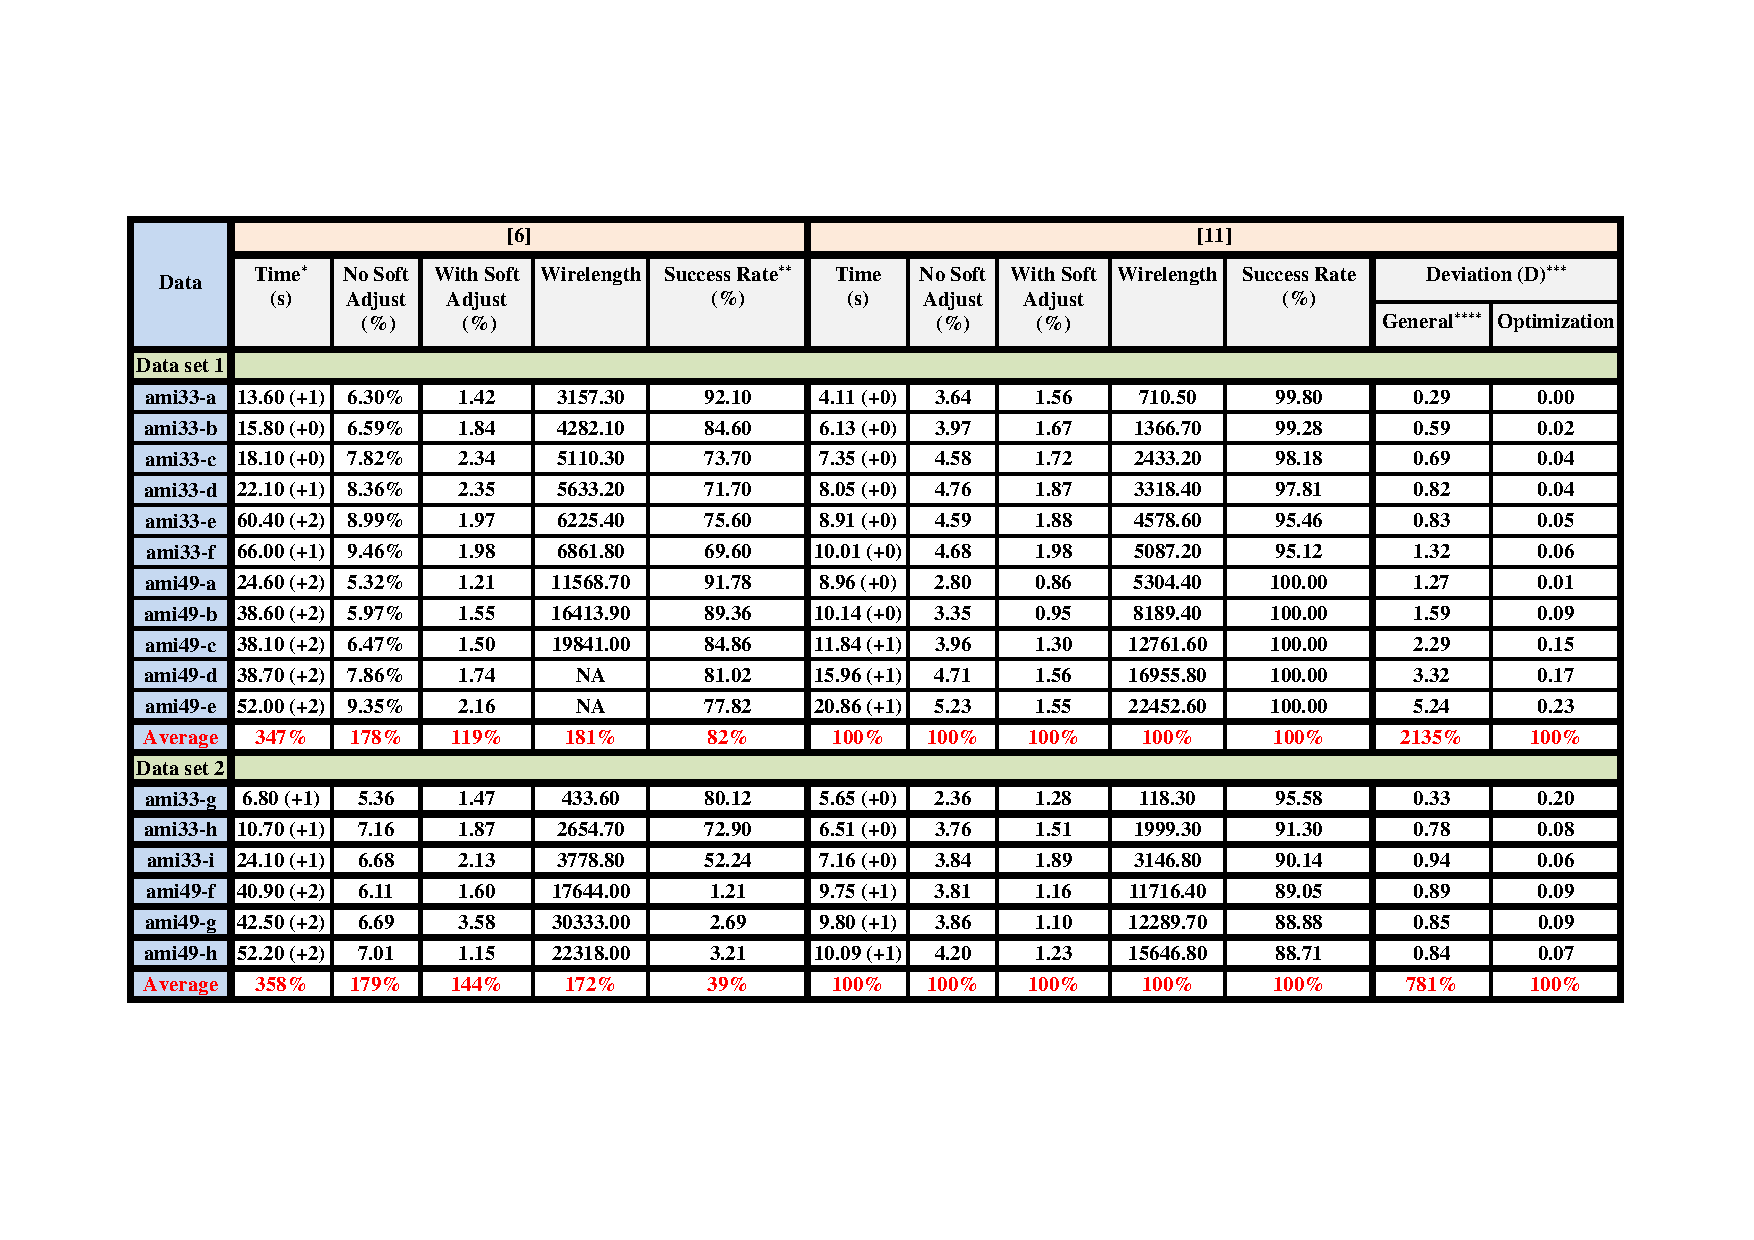
\includegraphics[width=17cm]{Fig/Table_2.pdf}}
    %\centerline{\psfig{figure=Fig/Table_2.eps, width=17cm}}\\
   $^*$Figures inside brackets represent the run time for soft module adjustment.\\
   $^{**}$The percentage of the floorplan generated by all iterations of the SA in which all the buses are feasible.\\
   $^{****}$The deviation (D) is obtained from total deviations at each load divided by total number of loads.\\
   $^{***}$The deviation at each load is estimated by total number of turning nodes from the driver to the load divided by total number of loads.
  \label{fig::TABLE_II}
\end{figure*}

In this section, we perform the experiments on the algorithm which
is published on GLSVLSI 2010 with the state-of-the-art bus-driven
floorplanner \cite{Ma08} which is published on ASPDAC 2008.
We implemented our bus-pin-aware bus-driven floorplanner in C
language on a 1.86-GHz Linux machine with 2GB memory. All
testcases are run by both our floorplanner and the
bus-driven floorplanner \cite{Ma08} on the same
machine. For fair comparison, each floorplanner runs ten times for
each testcase and the average is reported. Since the impact of the bus pin
is not considered in \cite{Ma08},
the bus pin of each module is not defined in the data set 1.
Therefore, we modify those testcases and assign the initial position
of each bus pin randomly.

In addition to perform experiments on data set 1 used in \cite{Ma08},
we also create data set 2 by modifying some testcases in data set 1 to
demonstrate the excellent routability of our algorithm. In data set
2, the bus width of each bus is wider than data set 1, i.e., it is more
difficult to obtain a feasible solution.
In each testcase, the first module of each bus is treated as the driver.
The details of all testcases are shown in Table I.

The first experiment is performed on data set 1, and the comparison results
are shown in Table II. As for the experiments about the
deviation of each module, for fair comparison, we only list the
average deviation (D) in the rightmost two columns for estimated and
optimized bus routing results from our floorplanner because
\cite{Ma08} does not consider the impact of the bus pins.
In this paper, we consider the diagonal connection
between two modules, it makes the bus shape more flexible, and the
size of the solution space is increased such that a better solution
can be obtained. Compared with \cite{Ma08}, the experimental
results show that our algorithm performs better in runtime by
3.47$\times$, success rate by 1.22$\times$, and reduced the
deadspace by 1.19$\times$. We also develop an algorithm to
reduce the wirelength, the experimental results show that our algorithm
performs better in wirelength by 1.81$\times$. By considering the
accumulated deviation during determining the position and
orientation of each bus pin, it can obtain better deviation at each load.
Experimental results show that the optimized deviation achieves 21.35$\times$
better than the estimated bus routing solution on average.
In our platform, \cite{Ma08}
does not generate a feasible final solution in ami49-d
and ami49-e, these testcases are ignored in wirelength
comparison. In other testcases, \cite{Ma08} fails to generate a
feasible final solution in some iterations of the ten annealing
processes, these iterations are also ignored in wirelength
comparison.

The experimental results of data set 2 are also shown in Table II.
Compared with \cite{Ma08}, the experimental results show that our
algorithm performs better in runtime by 3.58$\times$, success rate
by 2.56$\times$, and reduced the deadspace by 1.44$\times$. In
terms of wirelength, our algorithm performs better by 1.72$\times$.
With deviation optimization, the deviation achieves 7.81$\times$ better
than the estimated ones on average.
For ami49-f, ami49-g, and ami49-h, \cite{Ma08} could
not generate the feasible solution effectively. However, our
floorplanner still holds high solution quality in all aspects.
Some packing results are shown in Figure~\ref{fig::packing_result1}.

\begin{figure}[htb]
  \centering
  \centerline{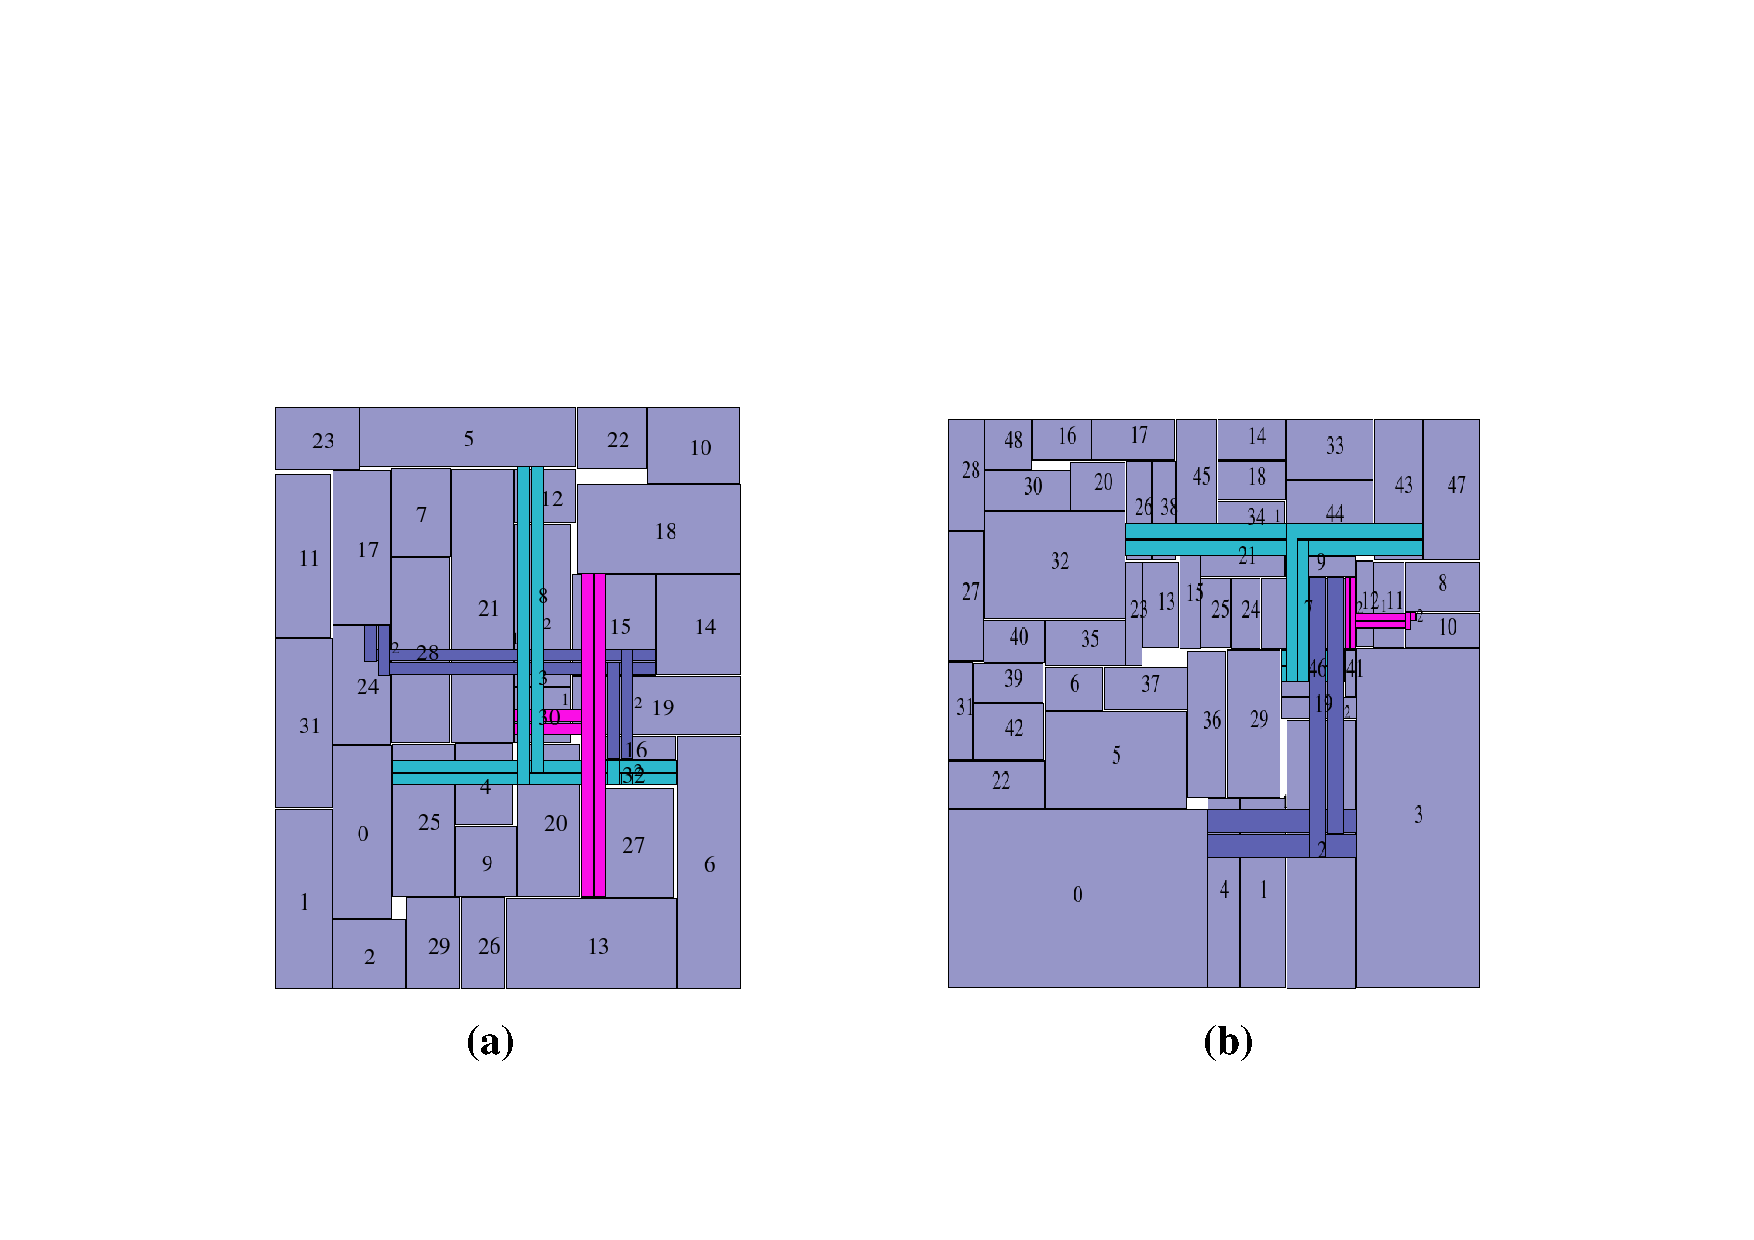
\includegraphics[width=11cm]{Fig/packing_result1.pdf}}
  %\centerline{\psfig{figure=Fig/packing_result1.eps, width=11cm}}
     \caption{
      (a) Packing result of ami33-i. The buses are \{13, 16, 18, 19, 21, 27, 30\}, \{0, 5, 6, 20, 25, 30, 32\},
                                                   \{14, 15, 16, 17, 24, 28, 32\}.
      (b) Packing result of ami49-h. The buses are \{7, 8, 9, 10, 11, 12, 41\}, \{29, 32, 41, 43, 44, 46, 47\},
                                                   \{0, 1, 2, 3, 4, 9, 46\}.
   }
  \label{fig::packing_result1}
\end{figure}

\begin{figure*}[htb]
{
  \centering
  \scriptsize
   TABLE III: COMPARISON BETWEEN \cite{PH10} AND THIS WORK
    \centerline{\includegraphics[width=17cm]{Fig/table_3.pdf}}\\
    %\centerline{\psfig{figure=Fig/table_3.eps, width=17cm}}\\
    $^*$The deviation at each load is estimated by total number of turning nodes from the driver to the load divided by total number of loads.\\
    $^{**}$The deviation (D) is obtained by the algorithm which is published in GLSVLSI 2010.\\
    $^{***}$The deviation (D) is obtained by the algorithm which is developed in this work.\\
  \label{fig::table3}
}
\end{figure*}

\section{The Comparison Between \cite{PH10} and This Work}
\label{sec::THE COMPARISON BETWEEN GLSVLSI 2010 AND THIS WORK}
In the remaining experiments, we are implemented our bus-driven floorplanner in C
language on a 2-GHz Linux machine with 16GB memory.
Since the work which is published on GLSVLSI 2010 only performs
the algorithm described in Section~\ref{sec::Deviation Minimization with Lookup Table Method}
after the SA, the deviation of each testcase could not
be minimized effectively. In this paper, we develop another efficient
approach to determine the deviation of each module such that
it can be integrated into the simulated annealing process.
The comparison results are shown in Table III.
Since the effect of the deviation is considered in this work during SA,
i.e., the solution space is much more constrained.
The run time is longer than GLSVLSI 2010 and the deadspace and wirelength are increased, however,
the deviation for each testcase can be further optimized to 0 as shown in the experimental results.

\section{The Comparison Between Modified \cite{PH10} and This Work}
\label{sec::The Comparison Between Modified GLSVLSI 2010 and This Work}
In this section, we modify the algorithm which is published in GLSVLSI 2010
such that it has the same structure with this work, i.e., the effect of
deviation is considered during SA.
The difference between the modified algorithm and this work is that
the algorithm described in Section ~\ref{sec::Deviation Minimization with Lookup Table Method}
is performed to determine the orientation of each bus pin in the modified algorithm, and
the algorithm described in ~\ref{sec::Fast Deviation Update Based on Topology Comparison}
is performed to determine the orientation of each bus pin in this work.
The comparison results are shown in Table IV.
The results show that deadspace, wirelength, success rate, and deviation is
nearly the same, nevertheless, the algorithm proposed in this paper is
run faster than the modified method.
Therefore, the proposed approach is more suitable on optimizing the
deviation during the SA.

\begin{figure*}[htb]
{
  \centering
  \scriptsize
   TABLE IV: COMPARISON BETWEEN MODIFIED \cite{PH10} AND THIS WORK
    \centerline{\includegraphics[width=17cm]{Fig/table_4.pdf}}\\
    %\centerline{\psfig{figure=Fig/table_4.eps, width=17cm}}\\
  \label{fig::table4}
}
\end{figure*}


\section{Experiments on Larger Testcases for \cite{PH10} and This Work}
\label{sec::EXPERIMENTS ON LARGER TESTCASES}

In this section, we will perform the experiments on larger testcases for the algorithm which is
published in GLSVLSI 2010 and this work.
The set of testcases are derived from n100, n200, n300 with bus sizes ranging from 10 to 40.
The details of all testcases are listed in Table V.
\begin{figure}[htb]
{
  \centering
  \scriptsize
   TABLE V: LARGER TESTCASE STATISTICS\\
   \centerline{\includegraphics[width=10cm]{Fig/table_5.pdf}}
   %\centerline{\psfig{figure=Fig/table_5.eps, width=10cm}}

  \label{fig::table5}
}
\end{figure}

\begin{figure*}[htb]
{
  \centering
  \scriptsize
   TABLE VI: COMPARISON BETWEEN \cite{PH10} AND THIS WORK ON LARGER TESTCASES
   \centerline{\includegraphics[width=17cm]{Fig/table_6.pdf}}\\
    %\centerline{\psfig{figure=Fig/table_6.eps, width=17cm}}\\
  \label{fig::table6}
}
\end{figure*}

To the best of our knowledge, no previous works can handle the buses with
such a large net size.
The comparison results are shown in Table VI.
The experimental results show that our algorithm performs better in success rate by 1.03$\times$,
deviation by 16.64$\times$, and reduces the deadspace 1.11$\times$.
Since it has to minimize the deviation during SA, it constrains the solution
space such that the bus wirelength are increased and spends more time on adjusting
the bus shape to obtain a better solution. However, the deviation can be further optimized to 0 in lots of
the testcases, and the deviation is effectively minimized in the difficult testcases.
Some packing results are shown in Figure~\ref{fig::packing_result2}.

\begin{figure}[htb]
  \centering
  \centerline{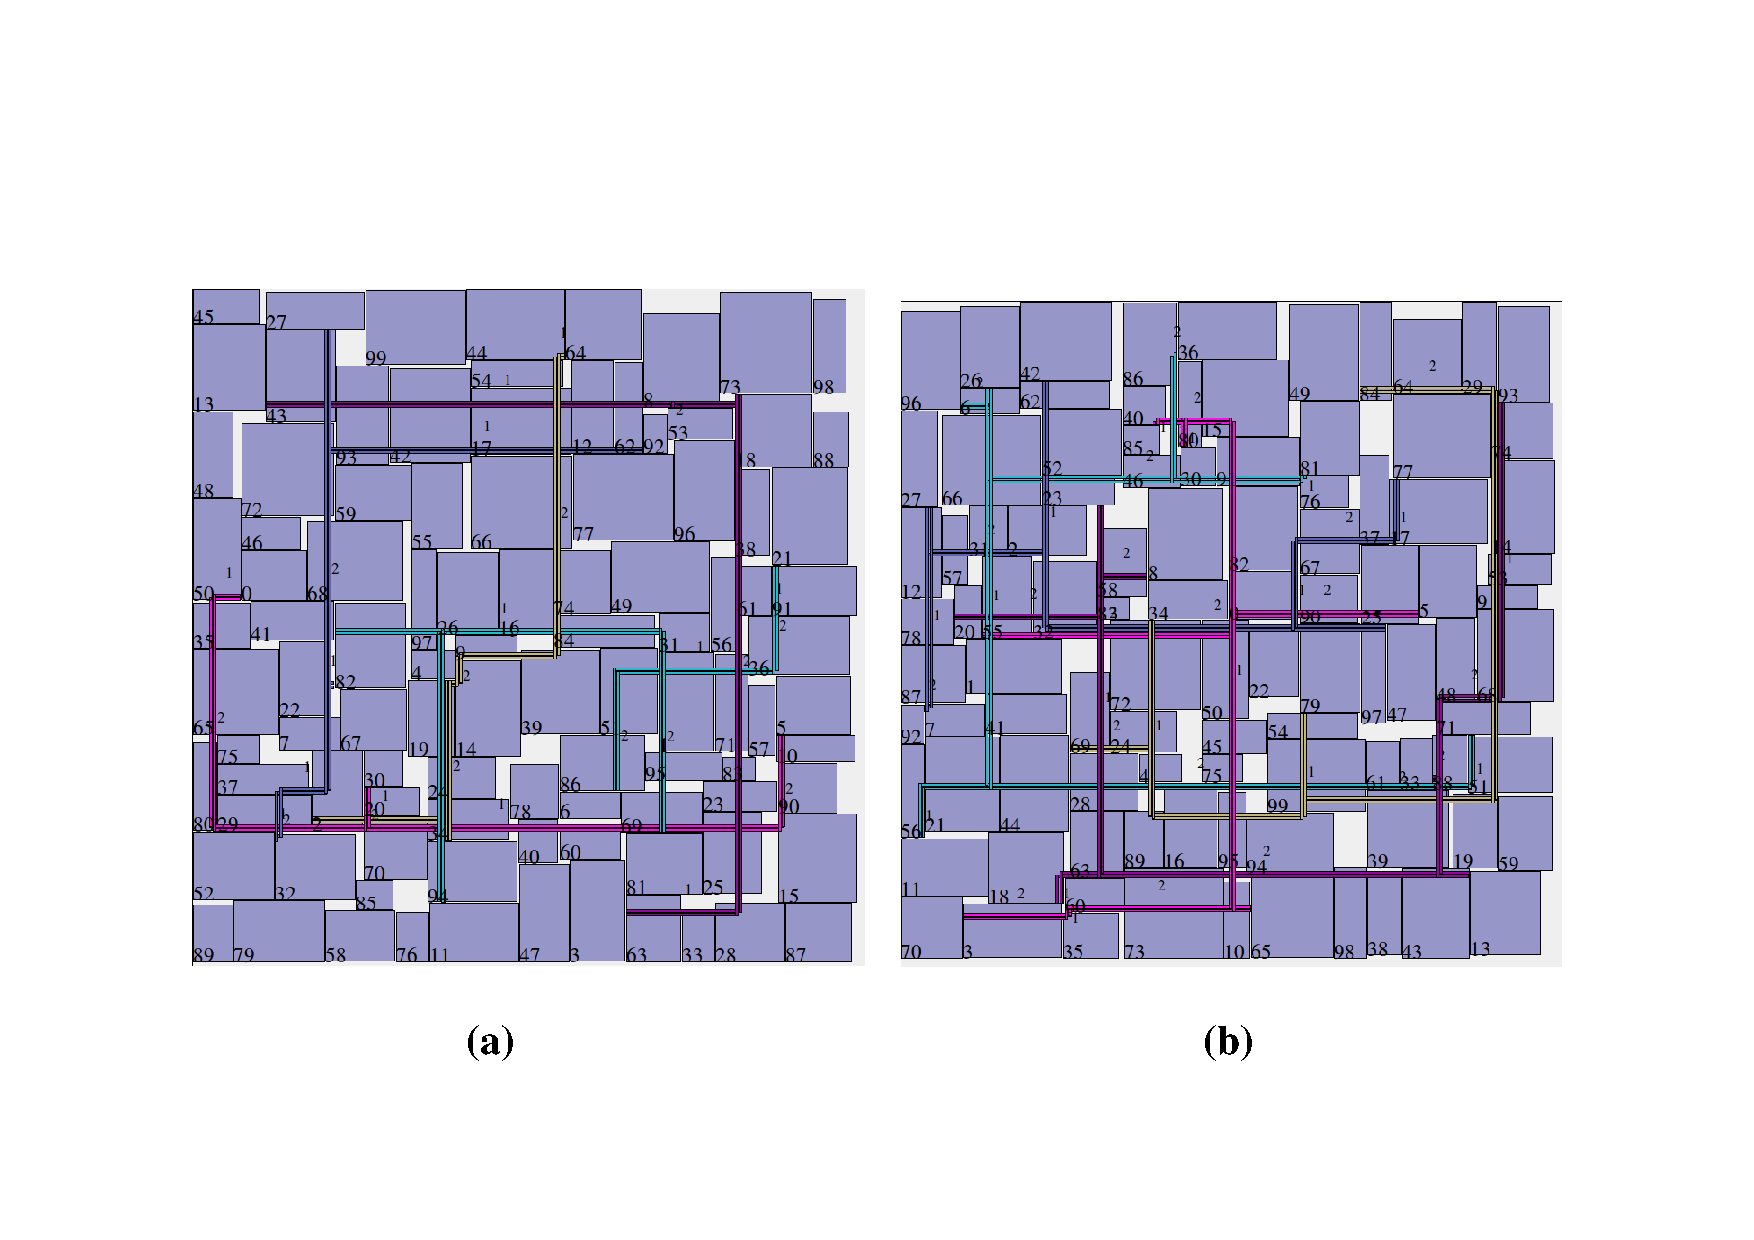
\includegraphics[width=13cm]{Fig/packing_result2.pdf}}
  %\centerline{\psfig{figure=Fig/packing_result2.eps, width=13cm}}
     \caption{
      (a) Packing result of n100-c. The buses are \{0, 10, 20, 30, 40, 50, 60, 70, 80, 90, 5, 15, 25, 35\},
                                                  \{1, 11, 21, 31, 41, 51, 61, 71, 81, 91, 6, 16, 26, 36\},
                                                  \{2, 12, 22, 32, 42, 52, 62, 72, 82, 92, 7, 17, 27, 37\},
                                                  \{3, 13, 23, 33, 43, 53, 63, 73, 83, 93, 8, 18, 28, 38\},
                                                  \{4, 14, 24, 34, 44, 54, 64, 74, 84, 94, 9, 19, 29, 39\}.
      (b) Packing result of n100-f. The buses are \{0, 10, 20, 30, 40, 50, 60, 70, 80, 90, 5, 15, 25, 35, 45, 55, 65, 75, 85, 95\},
                                                  \{1, 11, 21, 31, 41, 51, 61, 71, 81, 91, 6, 16, 26, 36, 46, 56, 66, 76, 86, 96\},
                                                  \{2, 12, 22, 32, 42, 52, 62, 72, 82, 92, 7, 17, 27, 37, 47, 57, 67, 77, 87, 97\},
                                                  \{3, 13, 23, 33, 43, 53, 63, 73, 83, 93, 8, 18, 28, 38, 48, 58, 68, 78, 88, 98\},
                                                  \{4, 14, 24, 34, 44, 54, 64, 74, 84, 94, 9, 19, 29, 39, 49, 59, 69, 79, 89, 99\}.
   }
  \label{fig::packing_result2}
\end{figure}


%%%%%%%%%%%%%%%%%%%%%%%%%%
\chapter{Conclusions}
\label{chap::CONCLUSIONS}
%%%%%%%%%%%%%%%%%%%%%%%%%%

\baselineskip=26pt

\hspace{5mm}As the early stage of
physical design, the floorplanning quality has dramatic impacts on
the chip performance. In this work, we proposed a high-quality
bus-driven floorplanning algorithm considering the practical
impacts of the bus pins. The experimental results show that our
floorplanner outperforms than the state-of-the-art floorplanner
\cite{Ma08} in all aspects. Besides, our algorithm can effectively
minimize the deviation in larger testcases.
The future work lies in extending our
algorithm to handle other practical constraints such as
fixed-outline, thermal effect, and etc.

%%%%%%%%%%%%%%%%%%%%%%%%%%
\chapter{Acknowledge}
\label{chap::ack}
%%%%%%%%%%%%%%%%%%%%%%%%%%

\baselineskip=26pt

\hspace{5mm}The authors would like to thank Tilen Ma and Prof. Evangeline F.Y. Young
of the Chinese University of Hong Kong for providing the authors with
benchmarks and program for the comparative studies.


%\appendix          % Appendix begins here
%\appendices            % If more than one appendix chapters,
%\appendices            % If more than one appendix chapters,

%\include{tex/appendix1}
%\include{tex/appendix2}

                                % use \appendices instead of \appendix
%\chapter{...}          % First appendix chapter, i.e., Appendix A.

%\section{...}          % This is appendix section A.1.


\begin{thebibliography}{200}
\bibitem{Rafiq02}
F. Rafiq, M. Chrzanowska-Jeske, H. H. Yang, and N. Sherwani,
``Integrated floorplanning with buffer/channel insertion for
bus-based microprocessor designs,'' {\it Proc. of ISPD}, pp.
56--61, 2002.

\bibitem{Xiang03}
H. Xiang, X. Tang, and Martin D. F. Wong, ``Bus-driven
floorplanning,'' {\it Proc. of ICCAD}, pp. 66--73, 2003.

\bibitem{Chen05}
T. C. Chen and Y. W. Chang, ``Modern floorplanning based on fast simulated
annealing,'' {\it Proc. of ISPD}, pp. 104--112, 2005.

\bibitem{Law05}
J. H. Y. Law and E. F. Y. Young, ``Multi-bend bus-driven
floorplanning,'' {\it Proc. of ISPD}, pp.113--120, 2005.

\bibitem{Xiang07}
H. Xiang, L. Deng, L.D. Huang, Martin D. F. Wong,
``OPC-friendly bus driven floorplanning,''
{\it Proc. of ISQED}, pp. 847--852, 2007.

\bibitem{Ma08}
T. Ma and E. F. Y. Young, ``TCG-based multi-bend bus-driven
floorplanning,'' {\it Proc. of ASPDAC}, pp. 192--197, 2008.

\bibitem{Kim08_1}
D. H. Kim and S. K. Lim,
``Global bus route optimization with application to microarchitectural design exploration,''
{\it Proc. of ICCD}, pp. 658--663, 2008.

\bibitem{Kim08_2}
D. H. Kim and S. K. Lim,
``Bus-aware microarchitectural floorplanning,''
{\it Proc. of ASPDAC}, pp. 204--208, 2008.

\bibitem{Sheng10}
W. Sheng, S. Dong, Y. Wu, and S. Goto,
``Fixed outline multi-bend bus driven floorplanning,''
{\it Proc. of ISQED}, pp. 632--637, 2010.

\bibitem{He10}
O. He, S. Dong, J. Bian, S. Goto, and C.K. Cheng,
``Bus via reduction based on floorplan revising,''
{\it Proc. of GLSVLSI}, pp. 9--14, 2010.

\bibitem{PH10}
B. S. Wu and T. Y. Ho,
``Bus-pin-aware bus-driven floorplanning,''
{\it Proc. of GLSVLSI}, pp. 27--32, 2010.

\bibitem{Mo07_1}
F. Mo and R. K. Brayton, ``Semi-detailed bus routing with
variation reduction,'' {\it Proc. of ISPD}, pp. 143--150, 2007.

\bibitem{Mo07_2}
F. Mo and R. K. Brayton, ``A simultaneous bus orientation and
bused pin flipping algorithm,'' {\it Proc. of ICCAD}, pp.
386--389, 2007.

\bibitem{Murata95}
H. Murata, K. Fujiyoshi, S. Nakatake, and Y. Kajitani,
``Rectangle-packing-based module placement,'' {\it Proc. of
ICCAD}, pp. 472--479, 1995.

\bibitem{Cormen01}
T. H. Cormen, C. E. Leiserson, R. L. Rivest, and C. Stein,
``Introduction to Algorithms,'' {\it 2nd ed., MIT Press and
McGraw-Hill Book Co.}, 2001.
\end{thebibliography}


%%%%%%%%%%%%%
% Vita page %
%%%%%%%%%%%%%

%\input{.mis/vita}

\end{document}
